\documentclass[
%draft,
ngerman,        % (ngerman/english) internationalisation
%  listoffigures,  % optional listings of figures, tables and listings
%  listoftables,
%  listoflistings,
%  twoside,        % double sided layout
]{iib_thesis}


\setlength\extrarowheight{3pt}
\usepackage{makecell}
\usepackage[inline]{enumitem}


\usepackage{textcomp}
\usepackage{float}

% breaks very long url
\def\UrlBreaks{\do\/\do-}
 
% norm
\newcommand\norm[1]{\left\lVert#1\right\rVert}

%\renewcommand{\tabularxcolumn}[1]{m{#1}}
\def\imagetop#1{\vtop{\null\hbox{#1}}}
% defines \RaggedRight
\usepackage{ragged2e}

\title{Pose Estimation in Gebäuden anhand von Convolutional Neural Networks und simulierten 3D-Daten}
\author{Abdullah Sahin}
\degree{Bachelor}
\studyprogram{Angewandte Informatik}
\date{3. September 2019}
\matno{108016202304}
\firstadviser{Prof. Dr.-Ing. Markus König}
\secondadviser{Patrick Herbers, M.\,Sc.}
\myabstract{
.....
}
\usetikzlibrary{spy,calc}



\newif\ifblackandwhitecycle
\gdef\patternnumber{0}

\pgfkeys{/tikz/.cd,
	zoombox paths/.style={
		draw=orange,
		very thick
	},
	black and white/.is choice,
	black and white/.default=static,
	black and white/static/.style={ 
		draw=white,   
		zoombox paths/.append style={
			draw=white,
			postaction={
				draw=black,
				loosely dashed
			}
		}
	},
	black and white/static/.code={
		\gdef\patternnumber{1}
	},
	black and white/cycle/.code={
		\blackandwhitecycletrue
		\gdef\patternnumber{1}
	},
	black and white pattern/.is choice,
	black and white pattern/0/.style={},
	black and white pattern/1/.style={    
		draw=white,
		postaction={
			draw=black,
			dash pattern=on 2pt off 2pt
		}
	},
	black and white pattern/2/.style={    
		draw=white,
		postaction={
			draw=black,
			dash pattern=on 4pt off 4pt
		}
	},
	black and white pattern/3/.style={    
		draw=white,
		postaction={
			draw=black,
			dash pattern=on 4pt off 4pt on 1pt off 4pt
		}
	},
	black and white pattern/4/.style={    
		draw=white,
		postaction={
			draw=black,
			dash pattern=on 4pt off 2pt on 2 pt off 2pt on 2 pt off 2pt
		}
	},
	zoomboxarray inner gap/.initial=5pt,
	zoomboxarray columns/.initial=2,
	zoomboxarray rows/.initial=2,
	subfigurename/.initial={},
	figurename/.initial={zoombox},
	zoomboxarray/.style={
		execute at begin picture={
			\begin{scope}[
				spy using outlines={%
					zoombox paths,
					width=\imagewidth / \pgfkeysvalueof{/tikz/zoomboxarray columns} - (\pgfkeysvalueof{/tikz/zoomboxarray columns} - 1) / \pgfkeysvalueof{/tikz/zoomboxarray columns} * \pgfkeysvalueof{/tikz/zoomboxarray inner gap} -\pgflinewidth,
					height=\imageheight / \pgfkeysvalueof{/tikz/zoomboxarray rows} - (\pgfkeysvalueof{/tikz/zoomboxarray rows} - 1) / \pgfkeysvalueof{/tikz/zoomboxarray rows} * \pgfkeysvalueof{/tikz/zoomboxarray inner gap}-\pgflinewidth,
					magnification=3,
					every spy on node/.style={
						zoombox paths
					},
					every spy in node/.style={
						zoombox paths
					}
				}
				]
			},
			execute at end picture={
			\end{scope}
			\node at (image.north) [anchor=north,inner sep=0pt] {\subcaptionbox{\label{\pgfkeysvalueof{/tikz/figurename}-image}}{\phantomimage}};
			\node at (zoomboxes container.north) [anchor=north,inner sep=0pt] {\subcaptionbox{\label{\pgfkeysvalueof{/tikz/figurename}-zoom}}{\phantomimage}};
			\gdef\patternnumber{0}
		},
		spymargin/.initial=0.5em,
		zoomboxes xshift/.initial=1,
		zoomboxes right/.code=\pgfkeys{/tikz/zoomboxes xshift=1},
		zoomboxes left/.code=\pgfkeys{/tikz/zoomboxes xshift=-1},
		zoomboxes yshift/.initial=0,
		zoomboxes above/.code={
			\pgfkeys{/tikz/zoomboxes yshift=1},
			\pgfkeys{/tikz/zoomboxes xshift=0}
		},
		zoomboxes below/.code={
			\pgfkeys{/tikz/zoomboxes yshift=-1},
			\pgfkeys{/tikz/zoomboxes xshift=0}
		},
		caption margin/.initial=4ex,
	},
	adjust caption spacing/.code={},
	image container/.style={
		inner sep=0pt,
		at=(image.north),
		anchor=north,
		adjust caption spacing
	},
	zoomboxes container/.style={
		inner sep=0pt,
		at=(image.north),
		anchor=north,
		name=zoomboxes container,
		xshift=\pgfkeysvalueof{/tikz/zoomboxes xshift}*(\imagewidth+\pgfkeysvalueof{/tikz/spymargin}),
		yshift=\pgfkeysvalueof{/tikz/zoomboxes yshift}*(\imageheight+\pgfkeysvalueof{/tikz/spymargin}+\pgfkeysvalueof{/tikz/caption margin}),
		adjust caption spacing
	},
	calculate dimensions/.code={
		\pgfpointdiff{\pgfpointanchor{image}{south west} }{\pgfpointanchor{image}{north east} }
		\pgfgetlastxy{\imagewidth}{\imageheight}
		\global\let\imagewidth=\imagewidth
		\global\let\imageheight=\imageheight
		\gdef\columncount{1}
		\gdef\rowcount{1}
		\gdef\zoomboxcount{1}
	},
	image node/.style={
		inner sep=0pt,
		name=image,
		anchor=south west,
		append after command={
			[calculate dimensions]
			node [image container,subfigurename=\pgfkeysvalueof{/tikz/figurename}-image] {\phantomimage}
			node [zoomboxes container,subfigurename=\pgfkeysvalueof{/tikz/figurename}-zoom] {\phantomimage}
		}
	},
	color code/.style={
		zoombox paths/.append style={draw=#1}
	},
	connect zoomboxes/.style={
		spy connection path={\draw[draw=none,zoombox paths] (tikzspyonnode) -- (tikzspyinnode);}
	},
	help grid code/.code={
		\begin{scope}[
			x={(image.south east)},
			y={(image.north west)},
			font=\footnotesize,
			help lines,
			overlay
			]
			\foreach \x in {0,1,...,9} { 
				\draw(\x/10,0) -- (\x/10,1);
				\node [anchor=north] at (\x/10,0) {0.\x};
			}
			\foreach \y in {0,1,...,9} {
				\draw(0,\y/10) -- (1,\y/10);                        \node [anchor=east] at (0,\y/10) {0.\y};
			}
		\end{scope}    
	},
	help grid/.style={
		append after command={
			[help grid code]
		}
	},
}

\newcommand\phantomimage{%
	\phantom{%
		\rule{\imagewidth}{\imageheight}%
	}%
}
\newcommand\zoombox[2][]{
	\begin{scope}[zoombox paths]
		\pgfmathsetmacro\xpos{
			(\columncount-1)*(\imagewidth / \pgfkeysvalueof{/tikz/zoomboxarray columns} + \pgfkeysvalueof{/tikz/zoomboxarray inner gap} / \pgfkeysvalueof{/tikz/zoomboxarray columns} ) + \pgflinewidth
		}
		\pgfmathsetmacro\ypos{
			(\rowcount-1)*( \imageheight / \pgfkeysvalueof{/tikz/zoomboxarray rows} + \pgfkeysvalueof{/tikz/zoomboxarray inner gap} / \pgfkeysvalueof{/tikz/zoomboxarray rows} ) + 0.5*\pgflinewidth
		}
		\edef\dospy{\noexpand\spy [
			#1,
			zoombox paths/.append style={
				black and white pattern=\patternnumber
			},
			every spy on node/.append style={#1},
			x=\imagewidth,
			y=\imageheight
			] on (#2) in node [anchor=north west] at ($(zoomboxes container.north west)+(\xpos pt,-\ypos pt)$);}
		\dospy
		\pgfmathtruncatemacro\pgfmathresult{ifthenelse(\columncount==\pgfkeysvalueof{/tikz/zoomboxarray columns},\rowcount+1,\rowcount)}
		\global\let\rowcount=\pgfmathresult
		\pgfmathtruncatemacro\pgfmathresult{ifthenelse(\columncount==\pgfkeysvalueof{/tikz/zoomboxarray columns},1,\columncount+1)}
		\global\let\columncount=\pgfmathresult
		\ifblackandwhitecycle
		\pgfmathtruncatemacro{\newpatternnumber}{\patternnumber+1}
		\global\edef\patternnumber{\newpatternnumber}
		\fi
	\end{scope}
}
%\includeonly{sections/section_1, sections/section_2, sections/section_4,sections/section_5 }
\begin{document}

% !TEX root = ../my_thesis.tex

\section{Einleitung}
Die Bestimmung der Pose (Position + Orientierung) von mobilen Geräten in Gebäuden verschafft im Bauwesen eine Reihe von Anwendungen wie z.B. die automatische Baufortschritterfassung sowie das Facility-Management und die Navigation über Augmented Reality \cite{kroppModelbasedPoseEstimation2016, kochNaturalMarkersAugmented2014}.
Während im Freien die mobilen Geräte über das \textit{Global Positioning System} (GPS) und die Mobilfunktechnologien lokalisiert werden können, ist grundsätzlich in Gebäuden und in der Abwesenheit von Satelliten- oder Funksignalen eine Lokalisierung über das GPS oder Mobilfunknetz nicht möglich \cite{yassinRecentAdvancesIndoor2016}. 

Für die Lokalisierung in Gebäuden gibt es verschiedene Verfahren, die sich an Technologien wie \textit{LIDAR, Ultra-Breitband, Wireless Access Point, Bluetooth Beacon etc.} bedienen. Darin stellt die visuelle Lokalisierung über eine Kamera die kostengünstigste und flexibelste Alternative dar, weil dieser keine flächendeckenden Hardwareinstallationen benötigt. Dies ist dadurch bedingt, dass heutzutage viele Menschen ein Smartphone mit einer hochauflösenden Kamera bei sich führen \cite{wuImagebasedCameraLocalization2018}.

Visuelle Lokalisierungsansätze wie z.B. die 
\textit{visuelle Odemetrie} (VO) oder das \textit{Simulta\-neous-Localization-and-Mapping} (SLAM) sind eingeschränkt auf die lokale Positionbestimmung. Daher benötigen diese Ansätze eine Ausgangsposition des Sensors, um die absolute Position in einem Gebäude zu lokalisieren \cite{stephenseGlobalLocalizationUsing2002}. Dieses Problem ist in der Literatur auch als das \textit{Kidnapped-Robot-Problem} (KRP) bekannt. KRP beschäftigt sich mit einem Roboter, der von seiner Umpositionierung uninformiert (\textit{entführt}) ist. Dieser soll über die Sensormessungen eigenständig seine globale Position in der Umgebung lokalisieren \cite{acharyaBIMPoseNetIndoorCamera2019}.


Die absolute Lokalisierung eines visuellen Abfragematerials ist über das Suchen eines korrespondierenden Bildes in einer Bildergalerie oder über die Regression der Pose anhand von Bild-Features möglich \cite{piascoSurveyVisualBasedLocalization2018}. Diese Verfahren benötigen entweder eine Datenbank aus Bildern mit bekannten Posen \cite{zhangImageBasedLocalization2006, arandjelovicThreeThingsEveryone2012} oder zusätzliche Daten wie die 3D-Punktwolke \cite{irscharaStructurefrommotionPointClouds2009, liWorldwidePoseEstimation2012} oder Tiefenbilder der Szene \cite{shottonSceneCoordinateRegression2013}. Allerdings ist die Beschaffung der Bilder und zusätzlichen Daten von allen möglichen Posen im Gebäude zeit- und kostenaufwendig \cite{acharyaBIMPoseNetIndoorCamera2019}.


Hierfür versuchen die \textit{Pose Estimation} Ansätze wie z.B. \textit{PoseNet} \cite{kendallPoseNetConvolutionalNetwork2015} mit \textit{künstlichen neuronalen Netzwerken} (KNN) eine geeignete Lösung zu bieten. PoseNet wird mit Datenpaaren bestehend aus RGB-Bildern und Posen trainiert, während die Ermittlung der Posen über das \textit{Structure-from-Motion} (SfM) einer Videoaufnahme der Umgebung genügt. Dennoch benötigen PoseNet und seine Nachfolger \cite{kendallModellingUncertaintyDeep2016, walchImageBasedLocalizationUsing2017, kendallGeometricLossFunctions2017, clarkVidLocDeepSpatioTemporal2017} Trainingsdaten durch das SfM der Videoaufnahmen, die den gesamten Innenraum der Gebäude abdecken. Die Aufnahme der Innenräume und das Erzeugen der Trainingsdaten über langsame und fehleranfällige SfM-Methoden ist zeitaufwändig und mühsam \cite{acharyaBIMPoseNetIndoorCamera2019}.

\citet{acharyaBIMPoseNetIndoorCamera2019} versuchten deshalb die Trainingsdaten aus der Simulation eines Gebäudes zu gewinnen. Dafür erzeugten die Forscher synthetische Bilder mit einer bekannten Pose entlang einer ca. 18$m$ langen Strecke in der 3D-Simulation eines Korridors. Trainiert auf dem PoseNet Modell mit den Gradientenbildern der synthetischen Daten konnten die Forscher \citet{acharyaBIMPoseNetIndoorCamera2019} bei der Evaluierung mit den Gradientenbildern der realen Daten eine Akkuratesse von ca. $2m$ in der Position und 7° in der Orientierung erzielen. 
%TODO: 2m kann durch lokale maßnahmen verbessert werden
Allerdings verlief die kurze Strecke überwiegend in einer Richtung und auf einer Etagenebene in der Simulation eines ca. $20m \times 5m \times 3m$ großen Korridors.


Ziel der vorliegenden Arbeit ist es, den Ansatz von \citet{acharyaBIMPoseNetIndoorCamera2019} in größeren Gebäudesimulationen und auf längeren Strecken, die einerseits in mehrere Richtungen verlaufen und andererseits sich auf mehreren Etagenebenen erstrecken, zu untersuchen. Um die Untersuchung bestmöglich an die Aufnahmestrecken und Gebäudesimulationen abhängig zu machen, wurde möglichst gleichermaßen wie in \cite{acharyaBIMPoseNetIndoorCamera2019} reale Evaluationsdaten erhoben, synthetische Trainingsdaten generiert und das PoseNet Modell mit den übereinstimmenden Hyperparametern verwendet.

Zusammenfassend wurde in der vorliegenden Arbeit Folgendes erreicht:
\begin{itemize}
	\item
	Insgesamt wurden vier Datensätze mit realen und synthetischen Daten aus den Innenräumen von zwei verschiedenen Gebäuden erhoben.
	\item 
	 Durch das Trainieren mit den Gradientenbildern der synthetischen Daten von Pose\-Net konnte geschlussfolgert werden, dass die Gradientenbilder der realen Evaluationsdaten auf einem begrenzten Gebäudeareal nur in eine Richtung bestimmt werden können.
\end{itemize}





Im weiteren Verlauf dieser Arbeit wird in Kapitel \ref{sec:kapitel_2} ein Überblick des Forschungsstandes vermittelt und die Grundlagen von künstlichen neuronalen Netzwerken behandelt. Insbesondere wird auf die \textit{Convolutional Neural Networks} eingegangen und die Netzwerkarchitektur von PoseNet vorgestellt, die in dieser Arbeit die Untersuchungsbasis darstellt. Im Anschluss daran wird in Kapitel \ref{sec:kapitel_3} die angewandte Methodik geschildert. Dort wird die Erhebung der Datensätze beschrieben und die Trainingsparameter der Untersuchungen angeben. Die Evaluationsergebnisse der trainierten KNNs werden in Kapitel \ref{sec:kapitel_4} präsentiert. Daraufhin werden in Kapitel \ref{sec:kapitel_5} die Ergebnisse diskutiert. Abschließend wird in Kapitel \ref{sec:kapitel_6} ein Fazit gezogen. 



% !TEX root = ../my_thesis.tex
\pagebreak
\section{Stand der Forschung und Grundlagen}

Dieses Kapitel versucht einen Überblick des Forschungsstandes in den unterschiedlichen Aspekten der Arbeit zu verschaffen. Anschließend vermittelt das Kapitel notwendige Grundkenntnisse.

\subsection{Einführung}


% SLAM, visual Odometrie, Viewpoint,

% Lokalisierungsproblem erläutern
% Ansätze aufzählen
% Überführen auf visuelle Lokalisierung
// Evt. Einblick über indoor Lokalizierungstechnicken \\

\textbf{Pose Estimation} wird in dieser Arbeit als eine Methode der visuellen Lokalisierung (\textit{Visual-Based Localization, kurz VBL}) betrachtet. VBL beschäftigt sich mit der Bestimmung der Pose (\textit{Position + Orientierung}) eines visuellen Abfragematerials (\textit{z.B. ein RGB-Bild}) in einer zuvor bekannten Szene  \cite{piascoSurveyVisualBasedLocalization2018}.
Ein naheliegendes Themengebiet der Robotik ist die visuelle Ortswiedererkennung (\textit{Visual Place Recognition, kurz VPR}) \cite{lowryVisualPlaceRecognition2016}. Die visuelle Ortswiedererkennung fokussiert sich auf das Feststellen eines bereits besuchten Ortes und definiert sich aus einer Mapping-, Datenverarbeitungs- und einem Orientierungsmodul. Allgemein lässt sich das Prozess eines VPRs folgend beschreiben. Eine interne Karte bekannter Orte wird durch das Mappingmodul verwaltet. Die Daten werden vom Datenverarbeitungsmodul vorbereitet und anschließend an das Orientierungsmodul übergeben. Daraufhin bestimmt das Orientierungsmodul die Pose und entscheidet mit der immer aktuell gehaltenen Karte, ob ein Ort bereits besucht wurde. Im Vergleich zur VPR versucht die visuelle Lokalisierung eine Pose zu bestimmen und benötigt daher neben den zwei Modulen kein Mappingmodul.

% hat 2 katogiren..
Die rein visuellen Methoden des VBLs unterteilen sich in indirekte und direkte Methoden \cite{lowryVisualPlaceRecognition2016}. Die indirekten Methoden behandeln das Lokalisierungsproblem als eine Bildersuche in einer Datenbank, ähnlich wie das \textit{Content Based Image Retrieval} \cite{lewContentbasedMultimediaInformation2006} Problem. Dabei wird das Abfragebild über eine Ähnlichkeitsfunktion mit den Vergleichsbildern aus der Datenbank abgeglichen \cite{zhangImageBasedLocalization2006, arandjelovicThreeThingsEveryone2012, radenovicCNNImageRetrieval2016}. Diese Art von Methoden benötigen eine sehr große Bildergalerie (\textit{Datenbank}) und liefern Ergebnisse bei Fund eines korrespondierenden Bildes \cite{lowryVisualPlaceRecognition2016}. Hingen versuchen die direkten Methoden die Pose über eine Referenzumgebung zu bestimmen und benötigen meist daher keine große Bildergalerie  \cite{piascoSurveyVisualBasedLocalization2018}. Es gibt drei Arten der direkten Methoden: 
\begin{enumerate*}[label=\arabic*)]
	\item Abgleichen von Features zu Punktwolken (\textit{z.B. \cite{liWorldwidePoseEstimation2012}})
	\item Pose Regression mit Tiefenbilder (\textit{z.B. \cite{shottonSceneCoordinateRegression2013a}})
	\item Pose Regression nur mit Bildern (\textit{z.B. \cite{kendallPoseNetConvolutionalNetwork2015}})
\end{enumerate*}

Die erste Art von Methoden versucht die Pose zu bestimmen, indem die 2D-3D Korrespondenz über das Abgleichen von Features des Abfragebildes gegen die Deskriptoren der 3D-Punkte hergestellt werden \cite{irscharaStructurefrommotionPointClouds2009, liWorldwidePoseEstimation2012, svarmCityScaleLocalizationCameras2017}. Diese Vorgehensweise hat Ähnlichkeiten zu den indirekten Methoden und benötigt statt einer Bildergalerie eine repräsentative 3D-Punktwolke der Szene \cite{piascoSurveyVisualBasedLocalization2018}. Die zweite Art von Methoden bestimmt anhand von Tiefenbilder die Pose z.B. über Regression Forests \cite{shottonSceneCoordinateRegression2013a}, Randomize Ferns \cite{glockerRealTimeRGBDCamera2015}, Coarse-to-Fine Registierung \cite{santosMappingIndoorSpaces2016} oder Neuronale Netze \cite{massicetiRandomForestsNeural2016}. Diese Forschungsprojekte liefern mit 3D-Bildern gewünschte Resultate. Die Ergebnisse sind abhängig von 3D-Kameras, diese sind jedoch nicht verbreitet.

\textbf{Convolutional Neural Networks} (\textit{CNN}) werden erfolgreich im Bereich des Maschinelles Sehens, wie z.B. bei der Klassifizierung von Bildern \cite{krizhevskyImageNetClassificationDeep2012, simonyanVeryDeepConvolutional2014, heDeepResidualLearning2015} sowie bei der Objekterkennung \cite{girshickRichFeatureHierarchies2013, renFasterRCNNRealTime2015b, girshickFastRCNN2015} eingesetzt. 
%Ein verbreiteter Ansatz beim Entwurf von CNNs ist das Modifizieren der vorhandenen sNetzwerkarchitekturen, die z.B. für die Bildklassifizierung angesichts der Wettbewerbe von ILSVRC \cite{russakovskyImageNetLargeScale2014} konstruiert wurden. Dieser Ansatz konnte beispielsweise erfolgreich in der Objekterkennung \cite{girshickFastRCNN2015}, Objektsegmentierung \cite{kokkinosPushingBoundariesBoundary2015, maninisConvolutionalOrientedBoundaries2016}, semantische Segmentierung \cite{nohLearningDeconvolutionNetwork2015, hazirbasFuseNetIncorporatingDepth2017a} und Tiefenbestimmung \cite{liDepthSurfaceNormal2015} verfolgt werden.
Seit Kurzem werden CNNs auch in den Anwendungsgebieten der Lokalisierung verwendet. Zum Beispiel verwenden  \citet{parisottoGlobalPoseEstimation2018} CNNs in Bezug auf das Simultaneous-Localization-and-Mapping (\textit{SLAM}) Problem. \citet{melekhovRelativeCameraPose2017} schätzen anhand CNNs die relative Pose zweier Kameras. \citet{costanteExploringRepresentationLearning2016} und \citet{wangDeepVOEndtoendVisual2017} setzen es im Bereich der visuellen Odometrie ein.

% Posenet überführen & erklären
Geleitet von den \textit{state-of-the-art} Lokalisierungsergebnissen der CNNs stellen \citet{kendallPoseNetConvolutionalNetwork2015} den ersten Ansatz zu direkten Posebestimmung nur mit RGB-Bildern vor. PoseNet ist die Modifikation der GoogLeNet \cite{szegedyGoingDeeperConvolutions2015} Architektur und zweckentfremdet es von der Bildklassifizierung zu einem Pose-Regressor. Trainiert mit einem Datensatz, bestehend aus Paaren von Farbbild und Pose, kann es die sechs Freiheitsgrade der Kamerapose in unbekannten Szenen mittels eines Bildes bestimmen. Dieser Ansatz benötigt weder eine durchsuchbare Bildgalerie noch eine Punktwolke oder Tiefenbilder der Szene. Im Vergleich zu den metrischen Ansätzen wie SLAM oder visuelle Odometrie liefert es eine weniger akkurate Pose. Es bietet jedoch eine hohe Toleranz gegenüber Skalierungs- und Erscheinungsänderungen des Anfragebildes an \cite{piascoSurveyVisualBasedLocalization2018}.

% Varianten aufzählen
Es gibt mehrere Ansätze, die die Genauigkeit von PoseNet übertreffen.
Einen Fortschritt erhalten die Autoren von PoseNet durch die hier \cite{kendallModellingUncertaintyDeep2015a} vorgestellte Anpassung ihres Models an einem Bayessian Neural Network \cite{denkerTransformingNeuralNetOutput1991, mackayPracticalBayesianFramework1991}.
Dieselben Autoren erweitern PoseNet mit einer neuen Kostenfunktion unter Berücksichtigung von geometrischen Eigenschaften \cite{kendallGeometricLossFunctions2017}. \citet{walchImagebasedLocalizationUsing2016} und \citet{clarkVidLocDeepSpatioTemporal2017} setzen Long-Short-Term-Memory (\textit{LSTM}) \cite{hochreiterLongShortTermMemory1997a} Einheiten ein, um Wissen aus der Korrelation von Bildsequenzen zu gewinnen. \citet{wuDelvingDeeperConvolutional2017} und \citet{naseerDeepRegressionMonocular2017} augmentieren den Trainingsdatensatz. \citet{wuDelvingDeeperConvolutional2017} stocken den vorhandenen Datensatz auf, indem sie die Bilder künstlich rotieren. \citet{naseerDeepRegressionMonocular2017} erweitern zuerst über ein weiteres CNN den Datensatz um Tiefenbildern. Anschließend simulieren die Autoren RGB-Bilder aus verschiedenen Viewpoints. Im Vergleich zu PoseNet verwenden \citet{mullerSQUEEZEPOSENETIMAGEBASED2017} und \citet{melekhovImageBasedLocalizationUsing2017} eine andere Architektur. 
Das Modell von \citet{mullerSQUEEZEPOSENETIMAGEBASED2017} basiert auf die SqueezeNet \cite{iandolaSqueezeNetAlexNetlevelAccuracy2016} Architektur. \citet{melekhovImageBasedLocalizationUsing2017} stellen HourglassNet, basierend auf einem symmetrischen Encoder-Decoder Architektur, vor. \citet{brahmbhattGeometryAwareLearningMaps2018} und \citet{valadaDeepAuxiliaryLearning2018, valadaIncorporatingSemanticGeometric} binden zusätzliche Informationen wie z.B. visuelle Odometrie, GPS oder IMU ein. 

Jedes dieser Ansätze benötigen annotierte Traininsdaten. Für die Erstellung solcher Daten wurden beispielsweise mit entsprechender Hardware ausgerüstete Trolleys \cite{huitlTUMindoorExtensiveImage2012}, 3D-Kameras \cite{izadiKinectFusionRealtime3D2011} oder SfM-Methoden \cite{kendallPoseNetConvolutionalNetwork2015} eingesetzt.

% Simulierte 3D-Daten 
\textbf{Simulierte 3D-Daten} werden in der Literatur oft eingesetzt, um das manuelle Erzeugen und Annotieren von Daten umzugehen. \citet{pishchulinArticulatedPeopleDetection2012a}, \citet{pengLearningDeepObject2014}, \citet{suRenderCNNViewpoint2015} und \citet{varolLearningSyntheticHumans2017} erzeugen ihren Trainingsdaten, indem sie virtuelle Objekte auf reale Hintergrundbildern platzieren. \citet{pishchulinArticulatedPeopleDetection2012a} generieren Daten zwecks Personenerkennung und Bestimmung derer körperlicher Pose. Zuvor werden auf den vorhandenen Bildern die körperliche Pose der Personen bestimmt und daran deren 3D Modelle rekonstruiert. Anschließend werden die 3D-Modelle in ihrer Pose variiert auf reale Hintergrundbildern platziert. Die Autoren konnten vergleichbare Ergebnisse zu den vorhandenen Ansätzen mit realen Daten ermitteln. \citet{pengLearningDeepObject2014} erstellen Daten, um Objekte auf realen Bildern zu detektieren. Von jeder Objektklasse werden 3D-Modelle auf einem Hintergrundbild aus einer Sammlung gelegt. Die Autoren stellen fest, dass das Feintunen mit synthetischen Daten eines Netzwerkes dann zu Abnahme der Akkuratesse führt, wenn das Netzwerk \textit{nur} für die Detektierung eines Objektes bestimmt ist. Hingegen konnten sie eine Steigung der Ergebnisse beim Trainieren mit simulierten Daten auf vortraniertem Netzwerk mit einer größeren Klassifierungskatalog ermitteln. \citet{suRenderCNNViewpoint2015} generieren einen großen Datensatz mit 3D-Modellen, um den Viewpoint von Objekten auf realen Bildern zu bestimmen. Bei dieser Datengenerierung wird jedes virtuelle Objekt auf zufällige Hintergrundbildern positioniert und mit unterschiedlichen Konfigurationen (\textit{z.B. Beleuchtung}) gerendert. Die Autoren konnten mit der Datenaugmentierung \textit{state-of-the-art} Viewport-Estimation Methoden zur \textit{PASCAL 3D+}\cite{xiangPASCALBenchmark3D2014} Benchmark übertreffen. \citet{varolLearningSyntheticHumans2017} erstellen künstliche Personen auf Bildern, um beispielsweise den menschlichen Körper in seine Glieder zu segmentieren. Dabei rendern sie zufällige virtuelle Personen mit zufälliger Pose auf beliebige Hintergrundbildern und konnten zeigen, dass die Akkuratesse einiger CNNs durch das Trainieren mit den erzeugten Daten steigt. \citet{fanelloLearningBeDepth2014} rendert künstliche Infrarotbilder von Händen sowie Gesichtern zwecks Tiefenerkennung und Segmentierung der Hand in den einzelnen Fingern sowie des Gesichtes in Bereiche aus einem RGB-Bild. Die Autoren konnten konventionelle Methoden über  Helligkeitsabfall übertreffen und vergleichbare Ergebnisse zu den Ansätzen mit einer herkömmlichen 3D-Kamera erzielen. \citet{dosovitskiyFlowNetLearningOptical2015} erlernen mit synthetischen Daten den optischen Fluss von Bildsequenzen.  Hierbei werden auf Hintergrundbildern aus einer Sammlung mehrmals bewegte virtuelle Stühle platziert. Die Autoren konnten mit syntethischen Daten \textit{state-of-the-art} Ansätze über reale Daten übertreffen.

Motiviert von der Datengenerierung über 3D-simulierten Daten stellt \citet{haImagebasedIndoorLocalization2018} einen Ansatz zur bildbasierte Lokalisierung in Gebäuden vor. Dieser Forschungsansatz generiert synthetische Daten aus einem Building-Information-Modeling (\textit{BIM}). Bei den Daten werden die durch das vortrainierte VGG Netzwerk \cite{simonyanVeryDeepConvolutional2014} extrahierte Features als wesentlich erachtet und in einer Datenbank gepflegt. Ein reales Aufnahmebild im Gebäude lässt sich durch den Vergleich der Features lokalisieren. \citet{acharyaBIMPoseNetIndoorCamera2019, acharyaMODELLINGUNCERTAINTYSINGLE2019} erzeugen ebenso Trainingsdaten aus einem BIM, jedoch verwenden sie zur Lokalisierung keine Datenbank bedürftiges Verfahren, sondern bestimmen die Pose direkt über PoseNet. Die Daten werden entlang einer ca. 30$m$ langem Flugbahn aus der Simulation eines ca. 230$m^2$  Korridors gesammelt. Hierbei werden sich in der Realitätstreue vom \begin{enumerate*}[label=\alph*)]
	\item karikaturistisch zu
	\item fotorealistisch hin über zu
	\item fotorealistisch-texturiert
\end{enumerate*} unterscheidende Daten erzeugt.
Traniert mit den unterschiedlichen synthetischen Daten, getestet auf die realen Daten, erzielen die Forscher eine Akkuratesse von
\begin{enumerate*}[label=\alph*)]
	\item 6,25$m$
	\item 5,99$m$
	\item 3,06$m$
\end{enumerate*}
 in der Position und  
 \begin{enumerate*}[label=\alph*)]
 	\item 37,16°
 	\item 11,33°
 	\item 12,25°
 \end{enumerate*}
 in der Orientierung.
Die besten Ergebnisse konnten die Autoren trainiert mit den 
\begin{enumerate*}[label=\alph*)]
	\addtocounter{enumi}{3}
	\item Gradienten- und
	\item Kantenbilder
\end{enumerate*} der karikaturistischen Daten, getestet auf die Gradientenbilder der realen Aufnahmen, erzielen. Die Autoren erhalten eine Akkuratesse von 
\begin{enumerate*}[label=\alph*)]
	\addtocounter{enumi}{3}
	\item 2,63$m$
	\item 1,88$m$
\end{enumerate*}
in der Position und  
 \begin{enumerate*}[label=\alph*)]
 	\addtocounter{enumi}{3}
	\item 6,99°
	\item 7,73°
\end{enumerate*}
in der Orientierung.
\\\\// Anbindung zu meinem Beitrag
\\\\
Im weiteren Verlauf des Kapitels werden einige grundlegende Themen erläutert. Zuerst werden künstliche neuronale Netze definiert. Danach wird ein elementares Wissen an Convolutional Neural Networks vermittelt und anschließend bekannte CNN Modelle näher erläutert.

%\subsection{Lineare Faltung}
%\subsubsection{Sobelfilter}
%\subsubsection{Gradientenbild}
%Bei der Erzeugung von Gradienten- bzw. Kantenbilder gehen einerseits wichtige Informationen im Hinblick auf das Ursprungsbild verloren, andererseits bleiben wichtige Informationen wie z.B. die geometrische Struktur erhalten.

\subsection{Künstliche neuronale Netzwerke}
\label{sec:KNN}
Künstliche neuronale Netze sind ein Forschungsgebiet der \textit{künstlichen Intelligenz} und imitieren die Beschaffenheit natürlicher neuronale Netze, um komplexe Probleme zu lösen. Inspiriert von ihren biologischen Vorbildern \footnote{das Nervensystem eines Lebewesen, z.B. des Menschen}, vernetzen künstliche neuronale Netzwerke (\textit{KNN}) künstliche Neuronen miteinander \cite{CS231nConvolutionalNeural}. Dabei kann die Verbindung unidirektional (\textit{feedforward}) oder bidirektional (\textit{feedback}) sein. 

Bei einem feedforward Netzwerk werden die Daten im Netz immer vorwärts übertragen, hingegen kann ein feedback Netzwerk, auch bekannt als \textit{Recurrent Neural Networks}, Daten rückwärts, sowie in einer Schleife zum selben Neuron, übergeben \cite{Goodfellow-et-al-2016}. Da feedback Netzwerke keinen Einsatz in dieser Arbeit haben, ist im weiteren Verlauf dieser Arbeit bei einem Netzwerk immer ein feedforward Ansatz gemeint. In diesem Kapitel werden als Nächstes ein künstliches Neuron definiert und anschließend ein feedforward Netzwerk beschrieben.


\subsubsection{Künstliches Neuron}
Ein einzelnes Neuron erhält einen Inputsignal auf mehreren Kanälen und löst erst ein Signal (\textit{output}) aus, falls die gewichtete Summe des Inputs einen gewissen Schwellwert erreicht \cite{CS231nConvolutionalNeural}. Abbildung \ref{fig:neuron} stellt eine beispielhafte Visualisierung eines künstlichen Neurons dar.

Ein künstliches Neuron mit der Inputgröße $M$ ist mathematisch die nicht-lineare Funktion $y : \mathbb{R}^M \mapsto \mathbb{R}$ mit dem Parameter $x$ als Input, $w$ als Gewichtsvektor, $b$ als ein Bias, $\phi$ als eine nicht-lineare \textit{Aktivierungsfunktion} \cite{CS231nConvolutionalNeural}:
\begin{equation}
	\label{eq:neuron}
	y(x)=\phi\left(\sum_{m=1}^{M} w_{i} x_{i} + b\right) = \phi(W^Tx+b)
\end{equation}

\vspace*{0.5cm}

\begin{figure}[H]
	\centering
	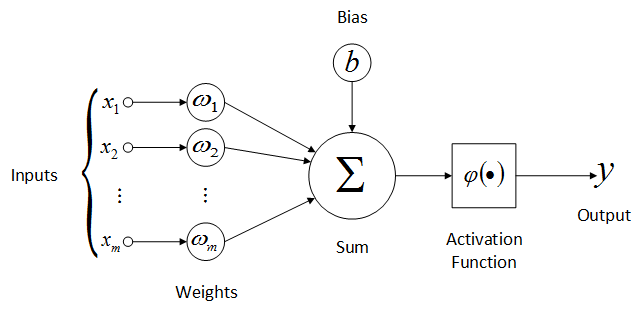
\includegraphics[width=0.8\textwidth]{images/neuron.png}
	\caption{Visualisierung eines künstlichen Neurons definiert nach der Gleichung \ref{eq:neuron}. Dieser Neuron summiert das Produkt des Inputvektors $x$  mit den jeweiligen Gewichten $w$ und addiert einen Bias $b$. Durch die Summe erzeugt die Aktivierungsfunktion $\phi$ das Output $y$ des Neurons. Entnommen aus \cite{deoliveiraSystemBasedArtificial2017}. }
	\label{fig:neuron}
\end{figure}

\subsubsection{Feedforward Neural Networks}
\label{sec:feedforwardNN}
Künstliche Neuronen können zu einer Schicht (\textit{layer}) zusammengeführt werden. Die Verbindung solcher Schichten bildet ein neuronales Netzwerk.
Bei einem feedforward (\textit{fully-connected}) Netzwerk übergibt jedes Neuron aus der Schicht $l$ seinen Output $y_{l}$ an jedem Neuron der Schicht $l+1$ weiter. Ebenso sind Neuronen aus der gleichen Schicht untereinander nicht verbunden \cite{Goodfellow-et-al-2016}.
Eine Schicht $l$ eines feedforward Netzwerkes operiert somit auf das Ouput $y_{l-1}$ und stellt die nicht-lineare Funktion $f_l :  \mathbb{R}^{M_{l-1}} \mapsto \mathbb{R}^{M_l}$ dar \cite{bauckhageInformedMachineLearning}:
\begin{equation}
\label{eq:layer}
y_l = f_l(y_{l-1}) = \phi(W^T_lx_{l-1}+b_{l})
\end{equation}


Die erste Schicht eines Netzwerk wird als Input-, die letzte Schicht als Ouput-Layer bezeichnet. Alle Schichten dazwischen sind Hidden-Layer \cite{Goodfellow-et-al-2016}. Der Ouput-Layer liefert zugleich auch das Ergebniss eines Netzwerks, daher haben die Neuronen des Ouput-Layers grundsätzlich keine Aktivierungsfunktion \cite{CS231nConvolutionalNeural}.

Die Tiefe (\textit{depth}) eines Netzwerks ist gegeben durch die Anzahl der Layer \footnote{der Input-Layer ist ausgeschloßen} und die Breite (\textit{width}) eines Layers wird durch die Anzahl der Neuronen bestimmt \cite{Goodfellow-et-al-2016}. 
Abilldung \ref{fig:neural_net} illustriert ein feedforward neuronales Netz als ein azyklischer Graph.

Ziel eines KNNs ist es eine Funktion $f^*$ zu approximieren, dass einen Input $x$ auf einen Output $y$ abbildet. Durch das Output $y$ kann das Input $x$ klassifiziert oder ein Wert regressiert werden. Sei $y = f(x; \theta)$  solch eine Funktion, dann besetzt ein KNN die Werte des $\theta$ Parameters mit eines der besten Approximierung. Der Parameter $\theta$ stellt hierbei die Gewichte dar, welche erlernt werden sollen \cite{Goodfellow-et-al-2016}. 
Das Lernen ist die strategische Anpassung der Gewichte über Input-Output Paare (\textit{Trainingsdaten}) und findet grundsätzlich durch ein \textit{Backpropagation}-Verfahren statt \cite{Goodfellow-et-al-2016}. 

Die Funktion $y = f(x; \theta)$ bildet sich aus den Funktionen der Schichten (Gleichung \ref{eq:layer}) im Netzwerk und kann bei einer Tiefe $L$ repräsentiert werden als die folgende Funktion $f :  \mathbb{R}^{M_0} \mapsto \mathbb{R}^{M_L}$ \cite{Goodfellow-et-al-2016, bauckhageInformedMachineLearning}:
 
\begin{equation}
\label{eq:network}
y = f(x; \theta)=  f_L(...f_2(f_1(x))) = (f_L \circ ... \circ f_2 \circ f_1)(x)
\end{equation}

\vspace*{1.5cm}

\begin{figure}[H]
	\centering
	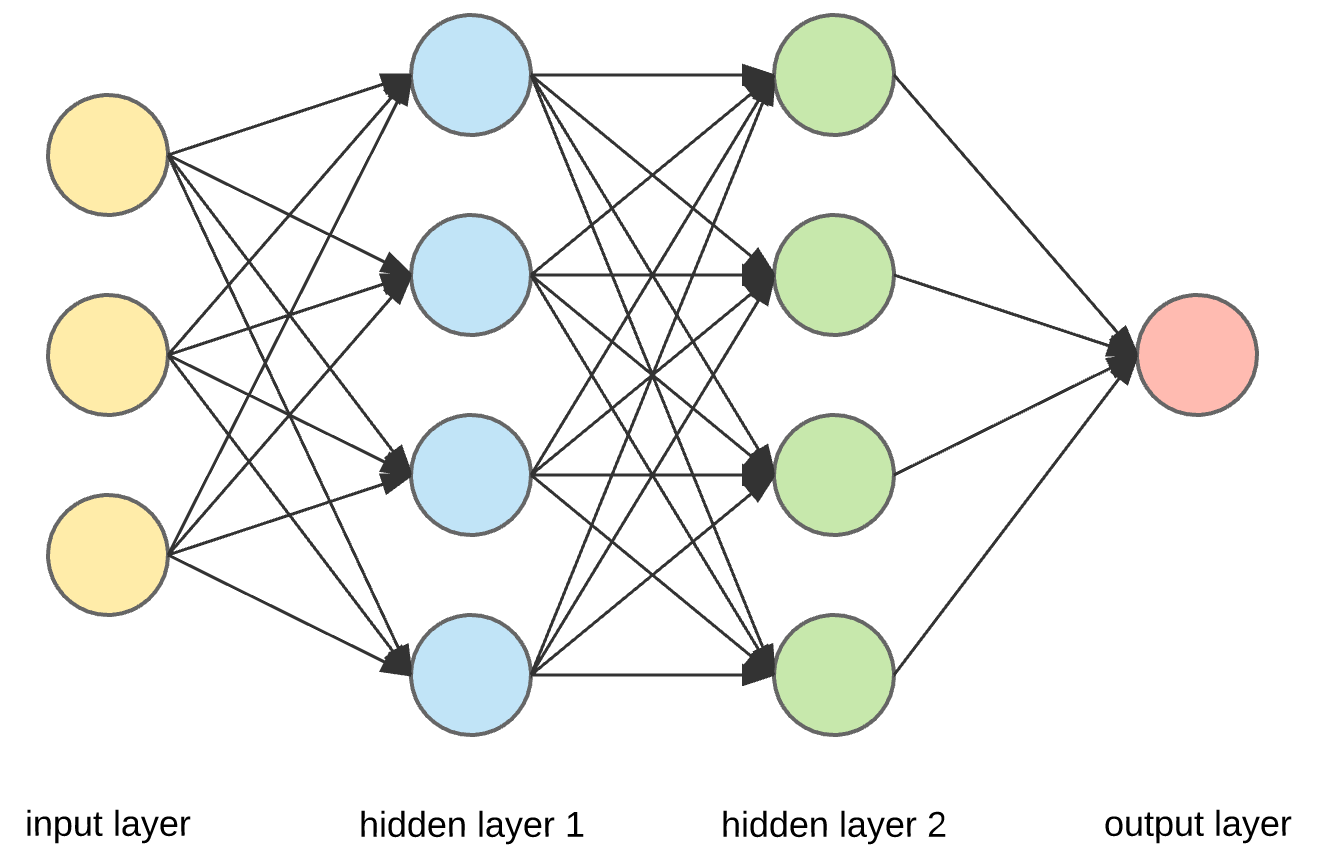
\includegraphics[width=0.75\textwidth]{images/neural_net.png}
	\caption{Ein feedforward neuronales Netz mit der Tiefe 3 bestehend aus einem Input-Layer der Breite 3, aus zwei Hidden-Layer der Breite 4 und einem Output-Layer der Breite 1. Mit der Gleichung \ref{eq:network}  lässt sich dieses Netzwerk als die Funktion $f :  \mathbb{R}^{3} \mapsto \mathbb{R}^{1}$ mit $f(x)=f_3(f_2(f_1(x)))$ darstellen. }
	\label{fig:neural_net}
\end{figure}
\vspace*{1.5cm}

\subsection{Convolutional Neural Networks}

Einfache neuronale Netze, wie sie in Abschnitt \ref{sec:KNN} beschrieben werden, arbeitet auf einem Inputvektor $x \in \mathbb{R}^{M}$. Hingegen arbeiten CNNs auf einem drei-dimensionalen Inputvolumen $x \in \mathbb{R}^{width} \times \mathbb{R}^{heigth} \times \mathbb{R}^{depth}$. CNNs werden hauptsächlich im Kontext von Bildern eingesetzt, dabei stellt z.B. ein 32 $\times$ 32 RGB-Bild ein Volumen von 32 $\times$ 32 $\times$ 3 dar \cite{CS231nConvolutionalNeurala}.

Eine Convolutional Neural Network Architektur setzt sich aus einer Sequenz von unterschiedlichen Layer-Arten zusammen \cite{CS231nConvolutionalNeurala}. Im weiteren Verlauf dieses Kapitels werden die Arten der Layer beschrieben. Tabelle \ref{tab:layer_param} gibt eine Übersicht der Layer und ihrer Parameter an.

\begin{table}[H]
	\centering
	\caption{Übersicht der Paramter und Hyperparamter der Layer eines Convolutional Neural Networks. Die Parameter werden während der Trainingsphase optimiert und Hyperparameter werden vorab fest definiert \cite{yamashitaConvolutionalNeuralNetworks2018}. }
	\begin{tabularx}{1.0\textwidth}{X X X}
		\textbf{Art des Layers} & \textbf{Parameter} & \textbf{Hyperparameter}\\
		\hline
		Convolutional Layer & Filter & \makecell[tl]{
			Anzahl der Filter\\
			Filtergröße\\
			Stride\\
			Padding\\
			Aktivierungsfunktion
		}\\
		\hline
		Pooling Layer &  \textit{keine}  & \makecell[tl]{
			Pooling Methode\\
			Filtergröße\\
			Stride\\
			Padding
		}\\
		\hline
		Fully-Connected Layer & Gewichte & \makecell[tl]{
			Anzahl der Gewichte\\
			Aktivierungsfunktion
		}\\
		\hline
	\end{tabularx}
	\label{tab:layer_param}
\end{table}

\subsubsection{Convolution Layer}
Der Convolutional Layer ist der Hauptbestandteil eines CNNs, welches die Kombination eines Convolution Operationen und einer Aktivierungsfunktion ist \cite{yamashitaConvolutionalNeuralNetworks2018}. 
Abbildung \ref{fig:convolution_layer} illustriert eine Convolution Operation. Abbildung \ref{fig:relu} stellt eine Aktivierungsfunktion dar.


\pagebreak
\vspace*{\fill}
\begin{figure}[H]
	\centering
	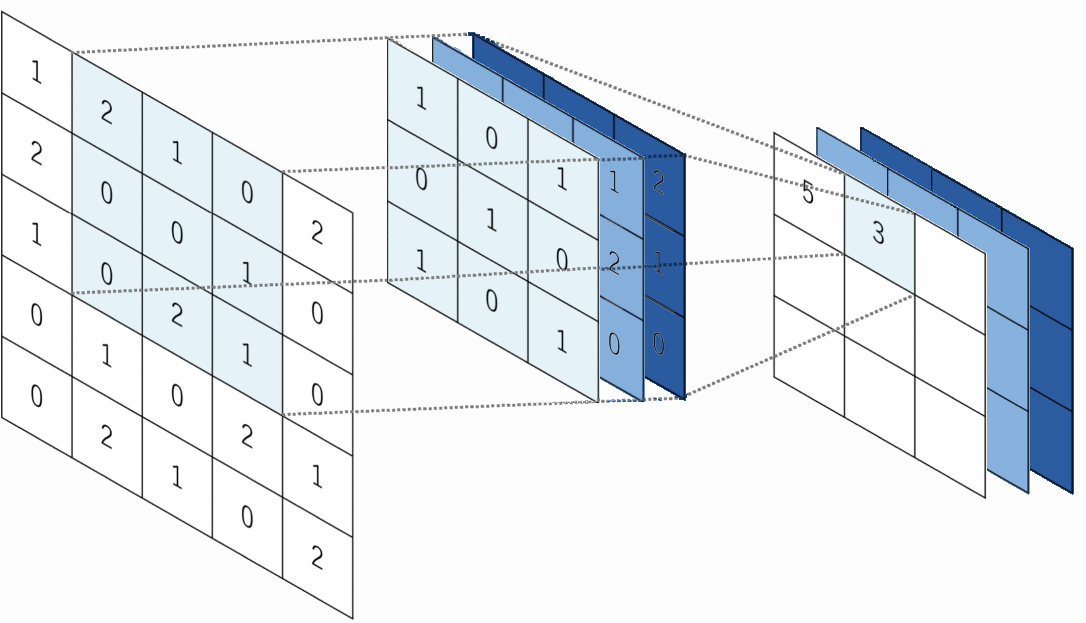
\includegraphics[width=0.7\textwidth]{images/convolution_layer.png}
	\caption{Ein Beispiel für die  Convolution Operation mit 3 Filtern der Größe 3 $\times$ 3, einem Stride von 1 und keinem Padding. Ein Filter bewegt sich entlang des gesamten Inputs mit der Schrittweite \textit{Stride} und bildet die Summe der elementweise multiplizierten Werte. Die Summe wird dann im Output an die korrespondierende Position geschrieben. Dieser Vorgang wiederholt sich für jedes Filter. \cite{yamashitaConvolutionalNeuralNetworks2018}. }
	\label{fig:convolution_layer}
\end{figure}

\begin{figure}[h]
	\centering
	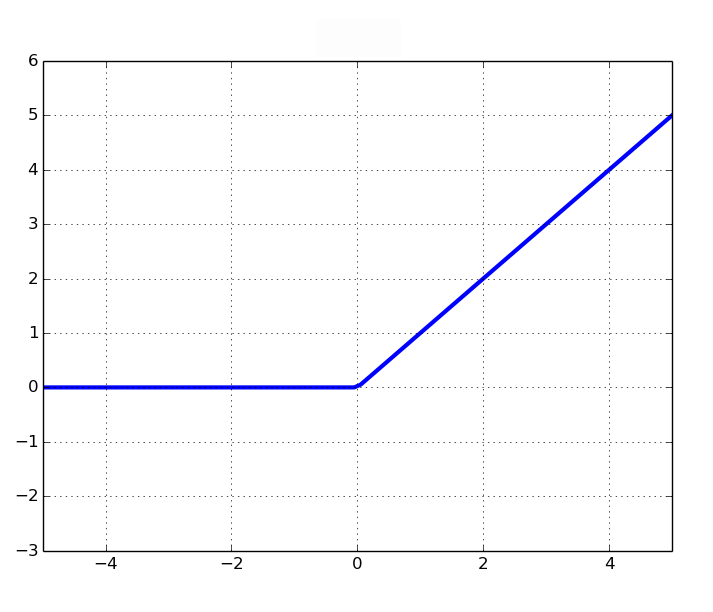
\includegraphics[width=0.4\textwidth]{images/ReLU.png}
	\caption{Ein Beispiel für eine Aktivierungsfunktion. Die ReLU (\textit{rectified liniear unit}) Aktivierungsfunktion wird typischerweise in CNNs eingesetzt und ist mathematisch definiert als: $f(x) = max(0,x)$ \cite{Goodfellow-et-al-2016} }
	\label{fig:relu}
\end{figure}

\subsubsection{Pooling Layer}
Auf einen Convolutional Layer folgt i.d.R. ein Pooling Layer. Pooling Layer reduzieren die Größe eines Inputvolumens und verringert somit die Anzahl der erlernbaren Parameter. Die Pooling Operation wird auf jeder Schicht der Eingabe ausgeführt \cite{CS231nConvolutionalNeurala}. Die meist verbreitete \textit{Pooling Methode} ist die Max-Pooling. Beim Max-Pooling iteriert ein Filter einer bestimmten Größe mit einer Schrittweite, gegeben durch dem Stride, über das Inputvolumen und extrahiert das Maximum im aktuellen Filterbereich. Das Maximum wird für die weitere Berechnung beibehalten und die restlichen Werte verworfen
 \cite{CS231nConvolutionalNeurala}. In dieser Arbeit wird neben der Max-Pooling Operation auch die Average-Pooling Operation eingesetzt. Das Average-Pooling behält im aktuellen Filterbereich den Durchschnittswert, statt das Maximum \cite{CS231nConvolutionalNeurala}.
 
 Im Vergleich zu einem Convolutional Layer wird ein Pooling Layer nur aus Hyperparameter definiert und bleibt daher statisch \cite{yamashitaConvolutionalNeuralNetworks2018}. Abbildung \ref{fig:pooling_layer} zeigt eine beispielhafte Ausführung einer Max-Pooling Operation. Tabelle \ref{tab:layer_param} listet die Hyperparameter eines Pooling Layers auf.
 \vspace*{1cm}
 \begin{figure}[H]
	\centering
	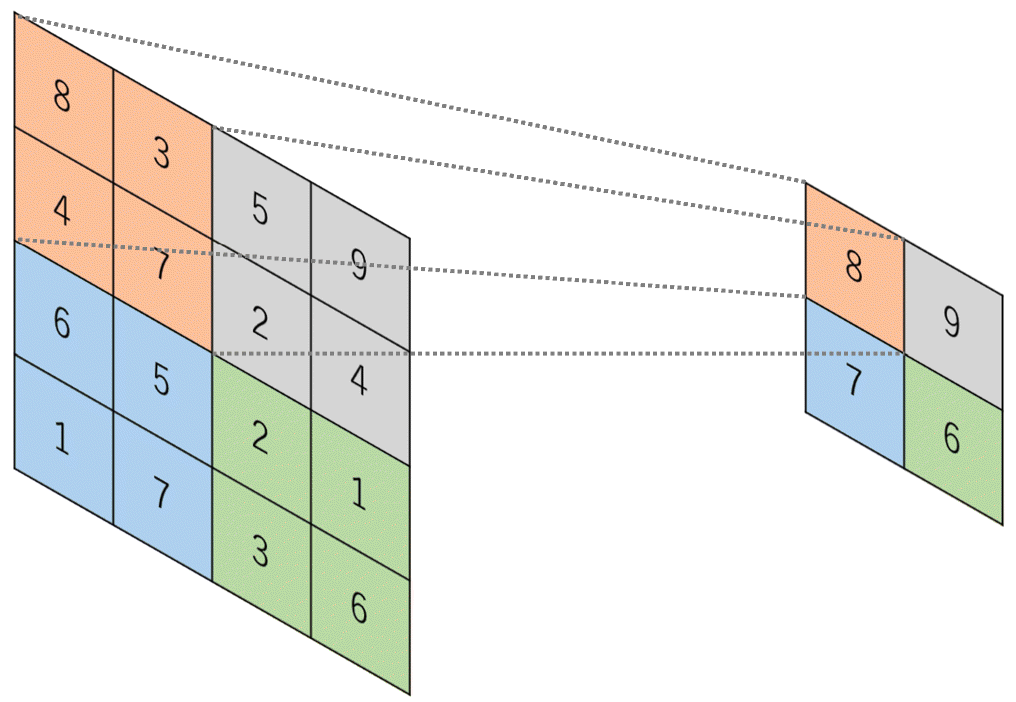
\includegraphics[width=0.6\textwidth]{images/max_pool.png}
	\caption{Ein Beispiel für eine Max-Pooling Operation mit einer Filtergröße von 2 $\times$ 2, einem Stride von 2 mit keinem Padding. In diesem Beispiel wird der Input in 2 $\times$ 2 Bereiche unterteilt und der Maximum jedes Bereiches als Output berechnet. Es werden die markantesten Werte einer Nachbarschaft behalten und der Rest verworfen. Diese Operation führt zu einer Reduzierung der Inputgröße um den Faktor 2. Entnommen aus \cite{yamashitaConvolutionalNeuralNetworks2018}.}
	\label{fig:pooling_layer}
\end{figure}



\subsubsection{Fully-Connected Layer}
Nach einer Periode von Convolution und Pooling Layer folgt meist eine fully-connected (\textit{FC}) Layer, auch bekannt als \textit{Dense Layer}. Dieser Layer folgt den gleichen Konzept der feedforward Neural Networks, wie in Abschnitt \ref{sec:feedforwardNN} beschrieben. Der Output dieses Layers wird häufig einer weiteren Aktivierungsfunktion übergeben \cite{yamashitaConvolutionalNeuralNetworks2018} und prinzipiell wird dadurch der Output des CNNs bestimmt.

\subsection{Bekannte CNN Modelle}
Es gibt zahlreiche bekannte CNN Modelle. Meist sind diese Modelle Sieger von internationalen Wettbewerben, solche wie die Large Scale Visual Recognition Challenge (\textit{ILSVRC}) \cite{russakovskyImageNetLargeScale2014}. Diese Arbeit behandelt nur das GoogLeNet Model und dessen Modifaktion PoseNet. 

\subsubsection{GoogLeNet}
\label{sec:googlenet}
GoogleNet wurde von \citet{szegedyGoingDeeperConvolutions2015} vorgestellt und gewann das ILSVRC14 Wettbewerb. In dem selben Paper stellen die Autoren das \textit{Inception Modul} dar.

 \begin{figure}[H]
	\centering
	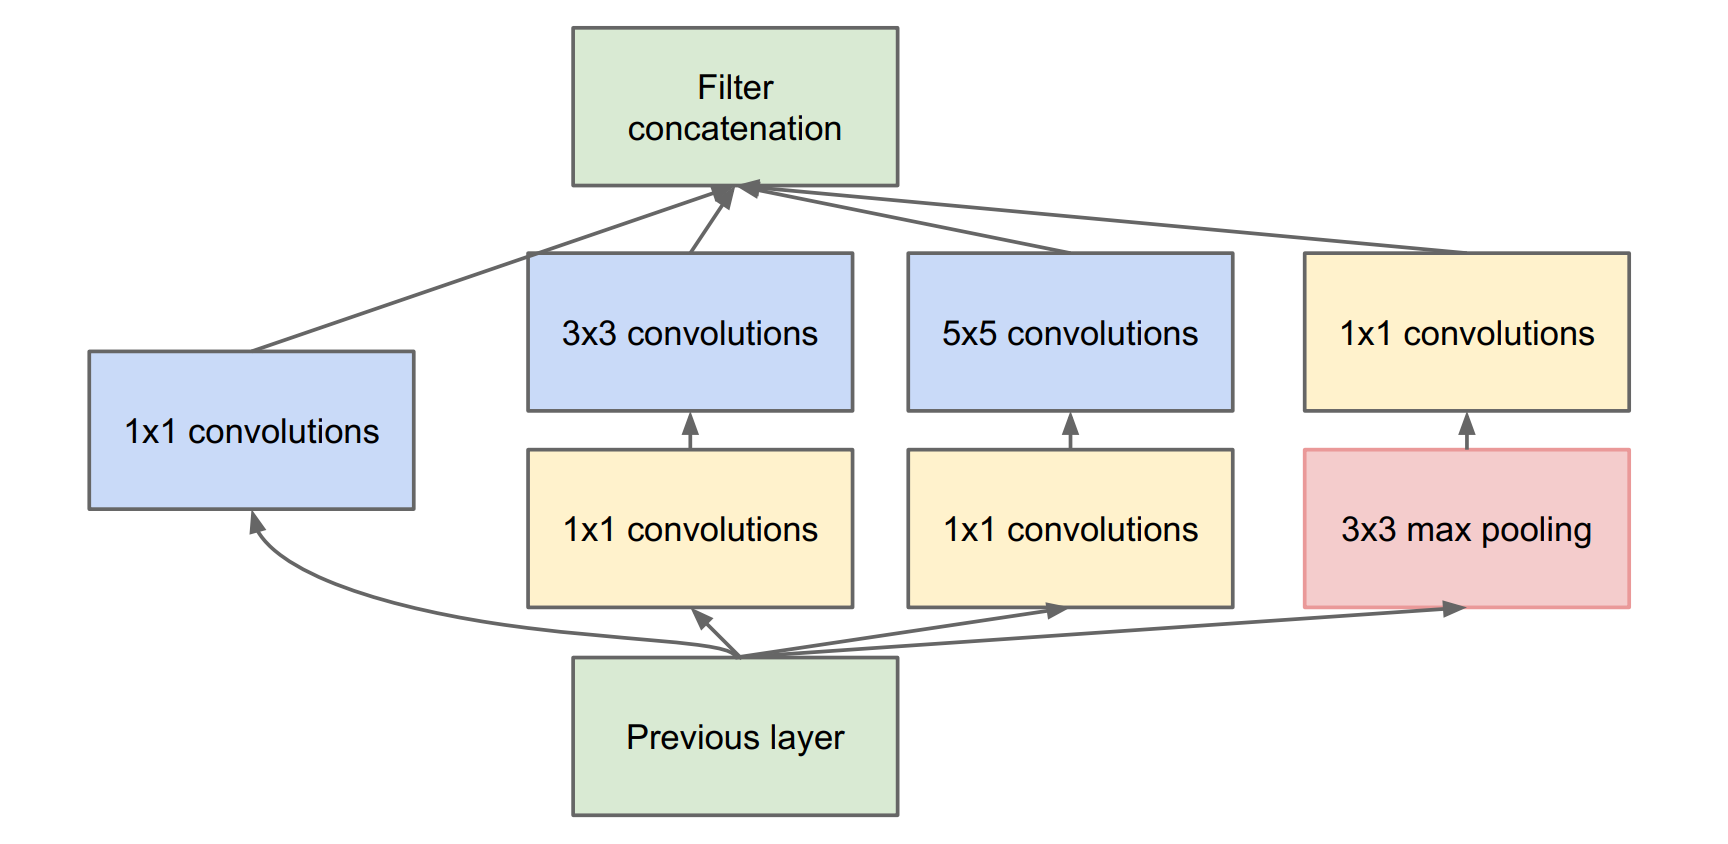
\includegraphics[width=0.8\textwidth]{images/googlenet/inception_module.png}
	\caption{Inception module. Entnommen aus \cite{szegedyGoingDeeperConvolutions2015}.}
	\label{fig:inception_module}
\end{figure}

\vspace*{\fill}
	 \begin{figure}[H]
		\centering
		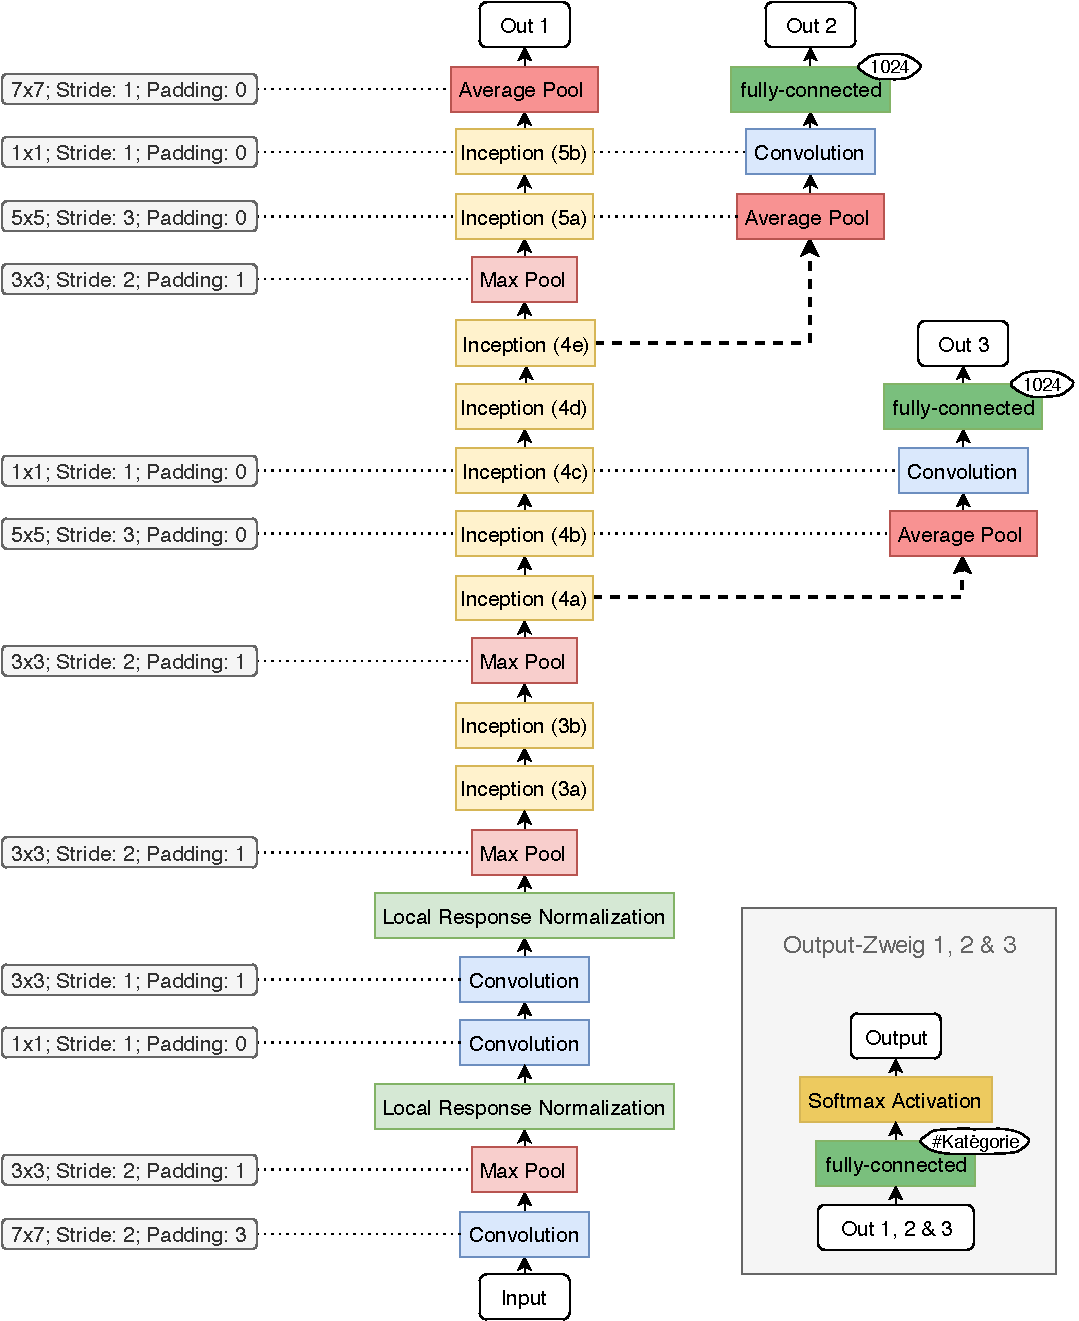
\includegraphics[width=0.85\textwidth]{images/googlenet/googlenet_diagram.pdf}
		\caption{Der architektonische Aufbau des GoogLeNet Models. Das Inception-Block wird in Abbildung \ref{fig:inception_module} detaillierter dargestellt. Es gibt 3 Ouput-Zweige, die mit einer identisch aufgebauten Output-Knoten enden. Die Werte der Output-Zweige 2 \& 3 haben nur während der Trainingsphase einen Einfluss und werden in der Evaluationsphase verworfen. In der Trainingsphase wird vor jedem Output-Knoten ein Dropout von 40\% angewandt. Jedes Convolution Layer hat die ReLU (Abbildung \ref{fig:relu}) als Aktivierungsfunktion. Die \textit{Local-Response-Normalization} \cite{krizhevskyImageNetClassificationDeep2012a} ist ein bekanntes Normierungsverfahren und kommt prinzipiell in Verbindung mit der ReLU Aktivierungsfunktion vor. Abbildung basiert auf \cite{szegedyGoingDeeperConvolutions2015}.}
		\label{fig:googlenet}
	\end{figure}
%\vspace*{\fill}
%\pagebreak
\subsubsection{PoseNet}
\label{sec:posenet}
PoseNet, vorgestellt von \citet{kendallPoseNetConvolutionalNetwork2015} im Jahr 2015, basiert auf die im Kapitel \ref{sec:googlenet} eingeführte GoogLeNet Architektur. Statt eine Wahrscheinlichkeitsverteilung der Klassifierungsergebnisse, liefert PoseNet die 6 Freiheitsgrade einer Pose $y = [\pmb{p};\pmb{q}]$, bestehend aus einem Positionsvektor $\pmb{p} \in  \mathbb{R}^{3}$ und eine Quaternion der Orientierung $ \pmb{q} \in  \mathbb{R}^{4}$.

PoseNet modifiziert die GoogLeNet Architektur an den Output-Knoten, dargestellt in Abbildung \ref{fig:googlenet}, wie folgt \cite{kendallPoseNetConvolutionalNetwork2015}:
\begin{itemize}
	\item Jedes der Softmax-Klassifikatoren werden ersetzt durch Regressoren. Dabei wird der Softmax-Activation Layer entfernt und der FC-Layer so modifiziert, dass es einen 7-dimensionalen Vektor\footnote{(3) für die Position und (4) für die Orientierung} ausgibt.
	\item Vor dem finalen Regressor des Output-Zweiges 1 wird ein weiteres FC-Layer der Breite 2048 eingefügt.

\end{itemize}
Abbildung \ref{fig:posenet_mods} veranschaulicht die Modifikation von GoogLeNet durch PoseNet.
\vspace*{1.2cm}
 \begin{figure}[H]
	\centering
	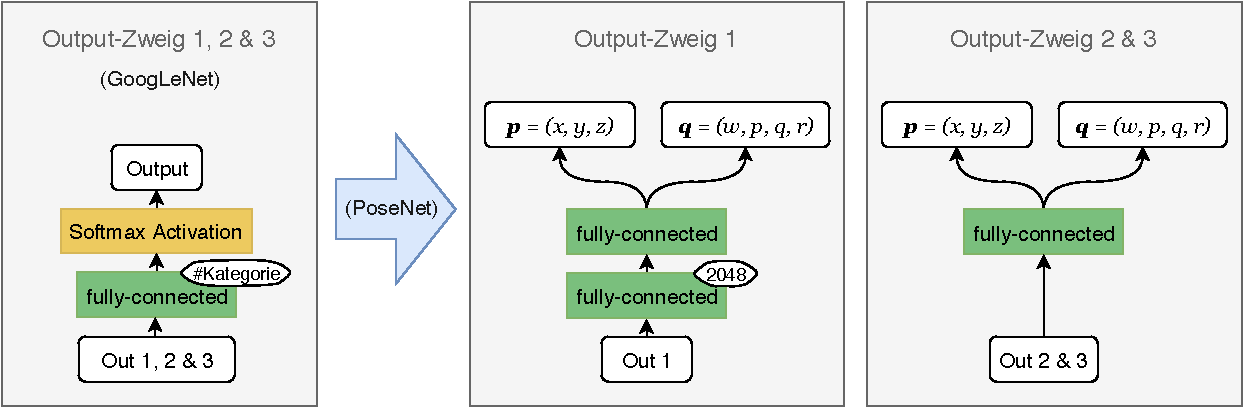
\includegraphics[width=\textwidth]{images/googlenet/posenet_diagram2.pdf}
	\caption{Veranschaulichung der Modifikation von den Output-Zweigen der GoogLeNet Architektur durch PoseNet. Die Softmax Aktivierungsfunktion sowie das fully-connected Layer mit Anzahl der Klassifizierungskategorien als Breite wurde von allen Output-Modulen entfernt. Jeder Output-Zweig hat einen FC-Regressionsschicht erhalten, welches die 6 Freiheitsgrade einer Pose bestimmt. Der Output-Zweig 1 wird zusätzlich mit einer weiteren FC-Layer der Breite 2048 vor dem Regressionsschicht erweitert \cite{kendallPoseNetConvolutionalNetwork2015}.}
	\label{fig:posenet_mods}
\end{figure}
\vspace*{1.5cm}

Die Autoren \citet{kendallPoseNetConvolutionalNetwork2015} stellen zusätzlich eine neue Kostenfunktion, mit den Parametern $\hat{y} = [\hat{\pmb{p}};\hat{\pmb{q}}]$ als Soll-Wert und $y = [\pmb{p};\pmb{q}]$ als Ist-Wert, vor:
\begin{equation}
	\label{eq:posenet_loss}
	loss(I) = \norm{ \hat{\pmb{p}} - \pmb{p} }_2 + \beta \norm{ \hat{\pmb{p}} - \frac{\pmb{q}}{\norm{\pmb{q}}}}_2
\end{equation}
Der Hyperparameter $\beta$ soll eine Balance der Kosten zwischen dem Positions- und Orientierungsdiskrepanz darstellen und wird in Gebäuden im Wertebereich zwischen 120 bis 750, sowie außerhalb des Gebäudes zwischen 250 bis 2000, empfohlen  \citet{kendallPoseNetConvolutionalNetwork2015}. 
% !TEX root = ../my_thesis.tex

\section{Methodik}
\label{sec:kapitel_3}

\begin{figure}[t]
	\centering
	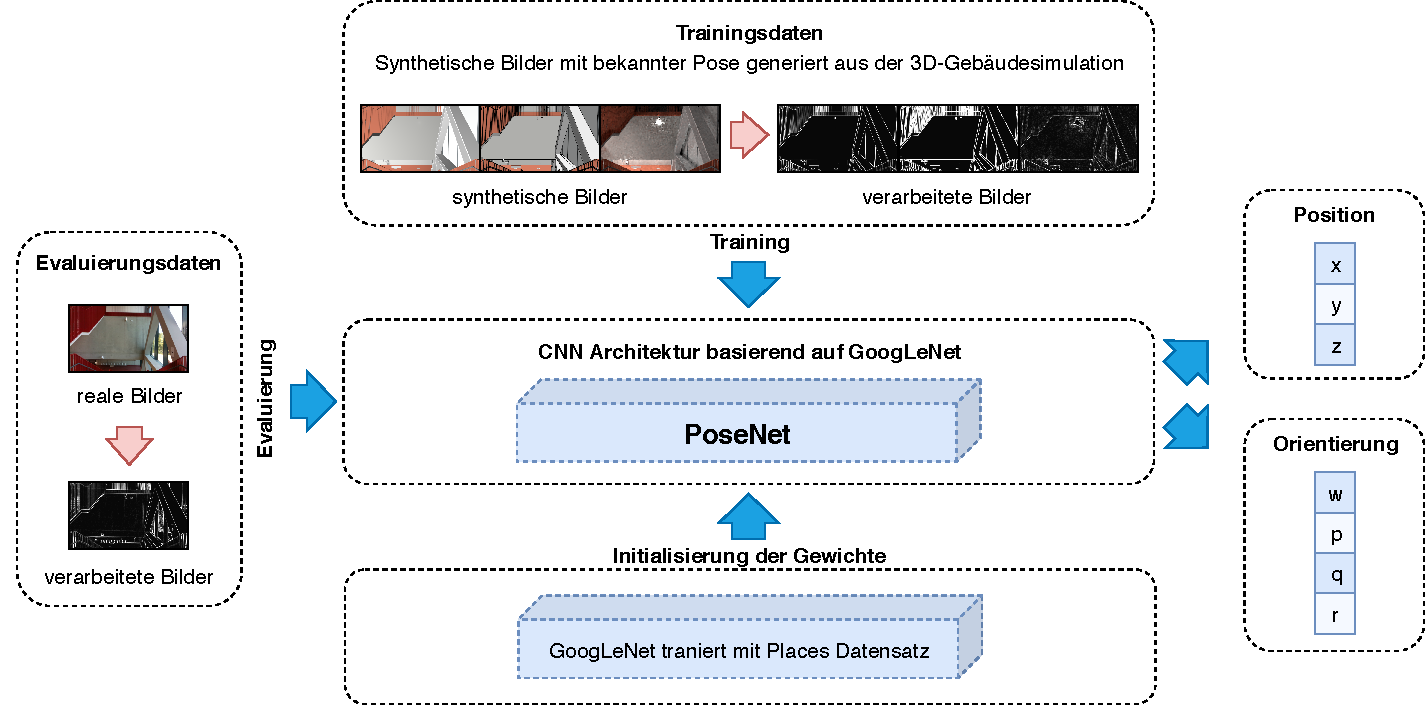
\includegraphics[width=0.9\textwidth]{images/methodik/methodik.pdf}
	\caption{Visualisierung der Methodik. Abbildung basiert auf \cite{acharyaBIMPoseNetIndoorCamera2019}.}
	\label{fig:methodik}
\end{figure}
Das vorliegende Kapitel gibt die Methodik dieser Arbeit wieder. Die Forscher \citet{acharyaBIMPoseNetIndoorCamera2019} konnten die Pose mit einer Akkuratesse von ca. $2m$ in der Position und 7° in der Orientierung auf einer ca. 18$m$ langen Strecke in einem ca. $20m \times 5m \times 3m$ großen Korridor bestimmen (s. Abb. \ref{fig:acharya_traj}). Dabei erhoben die Forscher reale Daten entlang des Korridors mit einem Smartphone  und bestimmten die korrespondierende Pose (\textit{Ground-Truth-Daten}) über SfM-Methoden. Daraufhin wurden entlang derselben Aufnahmestrecke in der 3D-Simulation des Korridors mehrere synthetische Daten generiert, die sich in ihrer Realitätstreue vom Karikaturistischen zum Fotorealistisch-texturierten variierten. Anschließend wurde das in Abschnitt \ref{sec:posenet} beschriebene PoseNet Modell mit Gradientenbildern der synthetischen Daten trainiert und mit Gradientenbildern der realen Daten evaluiert. Vorab wurde das PoseNet Modell mit den Gewichten eines Modells initialisiert, das auf der GoogLeNet Architektur mit dem Places Datensatz \cite{NIPS2014_5349} trainiert wurde \cite{acharyaBIMPoseNetIndoorCamera2019}. 

Die vorliegende Arbeit versucht den Ansatz von \citet{acharyaBIMPoseNetIndoorCamera2019} zur Pose Estimation in Gebäuden anhand von Convolutional Neural Network und simulierten 3D-Daten auf längeren Strecken in größeren Gebäudesimulationen zu untersuchen. Daher wurden zuerst entsprechende Datensätze erstellt und gleicherweise das PoseNet Modell trainiert sowie evaluiert. Um die Korrektheit des Training-Pipelines zu überprüfen wurden zuerst die Ergebnisse von \citet{acharyaBIMPoseNetIndoorCamera2019} reproduziert. Danach wurde das PoseNet Modell mit den Gradietenbildern der synthetischen Daten trainiert und evaluiert, um die Performance des Netzwerkes mit Trainings- sowie Evaluationsdaten derselben Domäne zu beobachten. Anschließend wurden zielgemäß die trainierten Netzwerke mit den Gradientenbildern der realen Daten evaluiert. Abbildung \ref{fig:methodik} visualisiert die Methodik dieser Arbeit.


Im weiteren Verlauf dieses Kapitels wird die Erhebung / Generierung der realen / synthetischen Daten beschrieben und die Verarbeitung der Daten dargestellt. Im Anschluss werden die Datensätze und die Trainingsparameter angegeben. 



\subsection{Erhebung der realen Daten}
\label{subsec:record_real_data}
In der Literatur wurden beliebige Kameras für die Aufnahme der realen Bilder verwendet und anschließend SfM-Methoden eingesetzt, um die Pose (\textit{Ground-Truth-Daten}) der realen Aufnahmen zu bestimmen \cite{kendallPoseNetConvolutionalNetwork2015, clarkVidLocDeepSpatioTemporal2017, acharyaBIMPoseNetIndoorCamera2019}. 
In der vorliegenden Arbeit wurde für die Bestimmung der Ground-Truth-Daten sowie die Aufnahme der Bilder zeitgleich zwei unterschiedliche Kameras der \textit{Intel Realsense} Reihe verwendet. Eine Intel Realsense T265\footnote{\url{https://www.intelrealsense.com/tracking-camera-t265/} (abgerufen am: 18.07.2019)} wurde eingesetzt. Diese verspricht bei gegebenen Bestkonditionen mit einer Abweichung von weniger als 1\% die relative Pose zum Ausgangspunkt über die SfM von zwei Fischaugenkameras (mit einer Auflösung von $848 \times 800$) und über IMU zu ermitteln. Zudem wurde eine Intel Realsense D435\footnote{ \url{https://www.intelrealsense.com/depth-camera-d435/} (abgerufen am: 18.07.2019)} eingesetzt, die eine 3D Punktwolke, ein $1280\times720$ Tiefenbild und ein $1920\times1080$ RGB-Bild einer Szene liefert. Die T265 wurde über die D435 montiert (s. Abb. \ref{fig:t265_d435}), um die RGB-Bilder der D435 mit den Ground-Truth-Daten der T265 annotieren zu können.

\begin{figure}
	\centering
	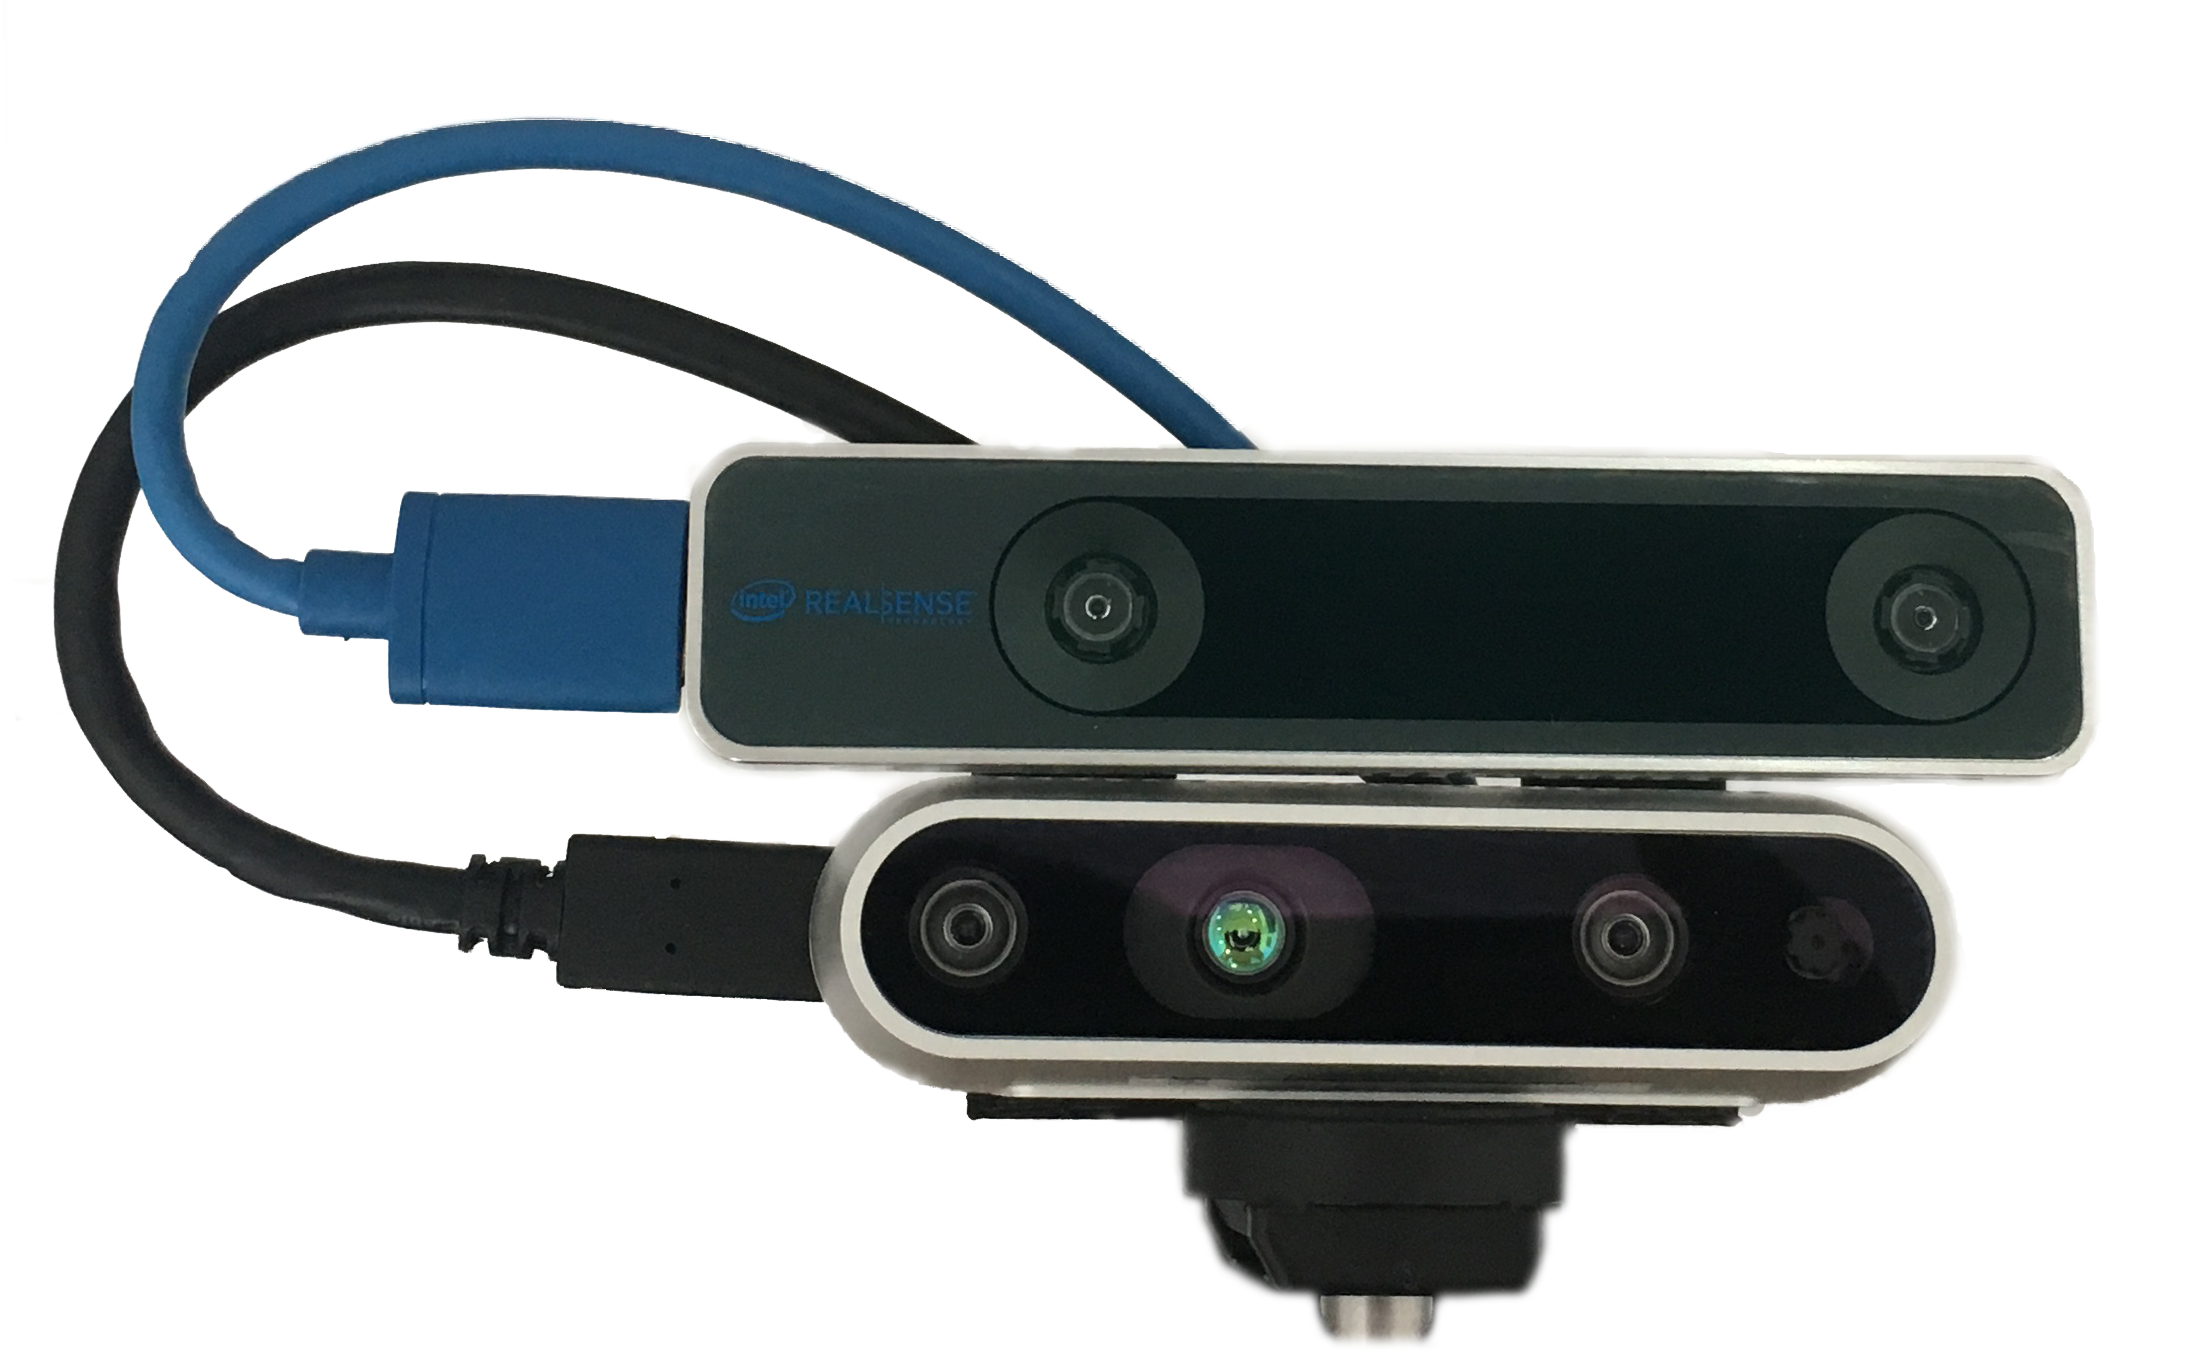
\includegraphics[width=0.5\textwidth]{images/real_dataset/t265_d435_2.png}
	\caption{Hardware für die Aufnahme der realen Daten. Die Intel Realsense T265 ist oberhalb der Intel Realsense D435 montiert.}
	\label{fig:t265_d435}
\end{figure}

In der Literatur wurden die realen Daten einer Zone grundsätzlich entlang einer Strecke aufgenommen \cite{kendallPoseNetConvolutionalNetwork2015, clarkVidLocDeepSpatioTemporal2017, acharyaBIMPoseNetIndoorCamera2019}. Daher wurden zuerst Aufnahmestrecken in den Gebäudesimulationen festgelegt und anschließend die Aufnahmen durchgeführt. Davor wurden die Ausgangspunkte der Aufnahmen zu einem Referenzpunkt in den Simulationen abgemessen und als Offset zur Bestimmung der globalen Position im Gebäude notiert.


Über das Robot Operating System\footnote{\url{https://www.ros.org/about-ros/} (abgerufen am: 18.07.2019)} (\textit{ROS}) Framework wurden die Kameras zeitgleich angesprochen und der Datenfluss der Kameras synchronisiert. Anschließend wurde der notierte Offset zur Bestimmung der absoluten Position im Gebäude zu den von der T265 berechneten zum Ausgangspunkt relativen Posen addiert. Somit beinhaltete jeder erhobene Datensatz ein Bild pro Fischaugenkamera, ein Tiefenbild, ein RGB-Bild, eine 3D Punktwolke und die dazugehörige absolute Pose im Gebäude pro Frame. Für die vorliegende Arbeit waren nur die Pose-Daten der T265 sowie die RGB-Bilder der D435 relevant, da PoseNet ausschließlich RGB-Bilder mit annotiertem Kamerapose benötigte. Abbildung \ref{fig:dataset} visualisiert ein Datensatzexemplar für einen Frame.

Aus Zeitgründen konnten die Bestkonditionen für die T265 nicht hergestellt werden, sodass die von der T265 berechneten Posen eine Abweichung (\textit{Drift}) bis zur 5\% (vgl. Abb. \ref{fig:trajectories}) aufweisen. Die Abweichung der Posen wurden nicht korrigiert, da in der vorliegenden Arbeit die realen Daten zur Evaluierung eingesetzt wurden, allenfalls für die Bestimmung eines Hyperparameters zwecks der Evaluation mit den realen Daten ein KNN trainiert wurde, sowie die Akkuratesse im Meterbereich für eine Beobachtung ausreichen sollte.


\begin{figure}
	\centering
	\begin{subfigure}[t]{0.3\linewidth}
		\centering
		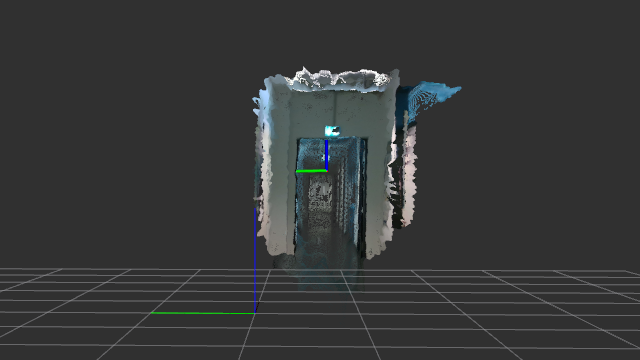
\includegraphics[width=\linewidth]{images/real_dataset/pointcloud3.png}
		\caption{Pose (T265) + \\ 3D Punktwolke (D435)}
		\label{subfig:odom1}
	\end{subfigure}
	\hfill
	\begin{subfigure}[t]{0.3\linewidth}
		\centering
		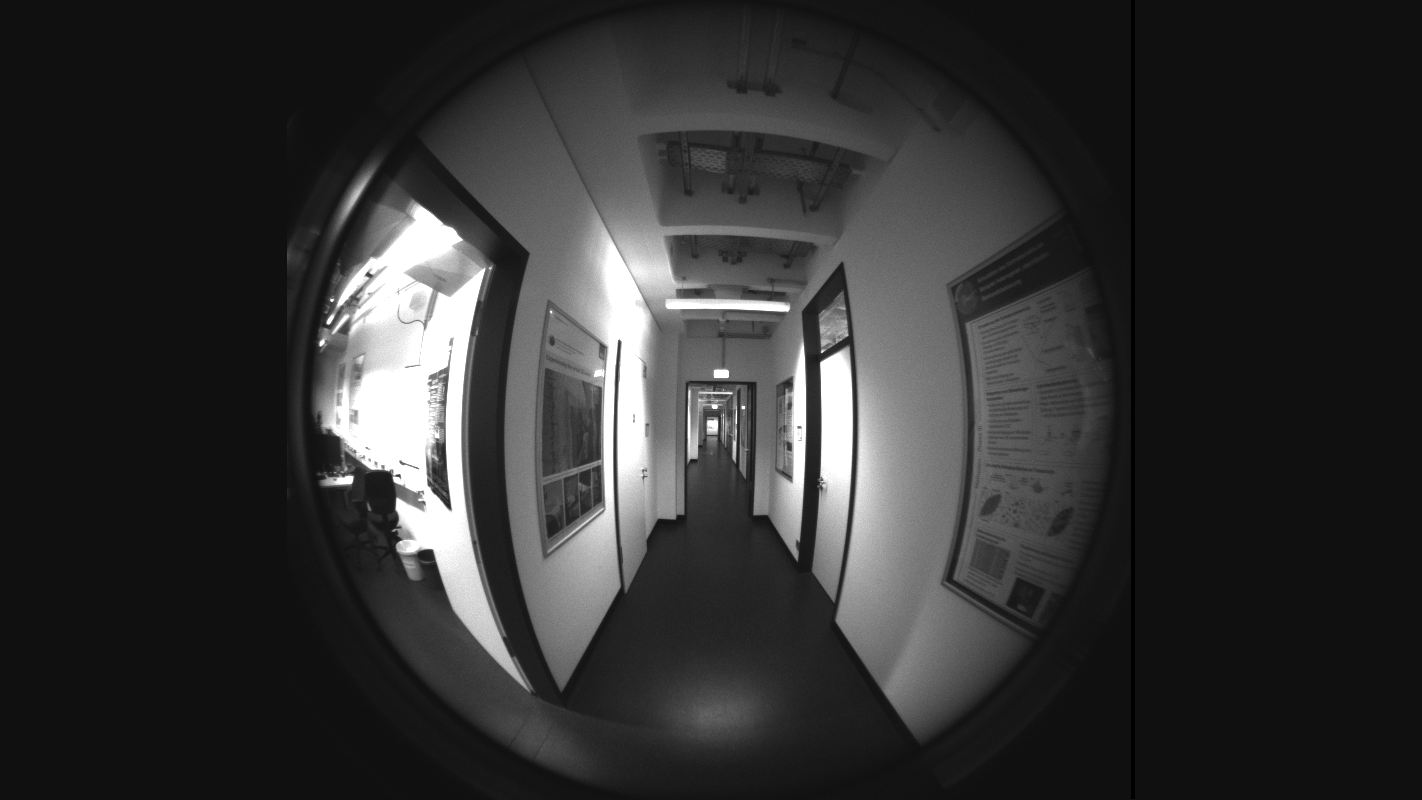
\includegraphics[width=\linewidth]{images/real_dataset/f1_frame000005.png}
		\caption{Fischaugenkamera 1 \\ (T265)}
		\label{subfig:fisheye1}
	\end{subfigure}
	\hfill
	\begin{subfigure}[t]{0.3\linewidth}
		\centering
		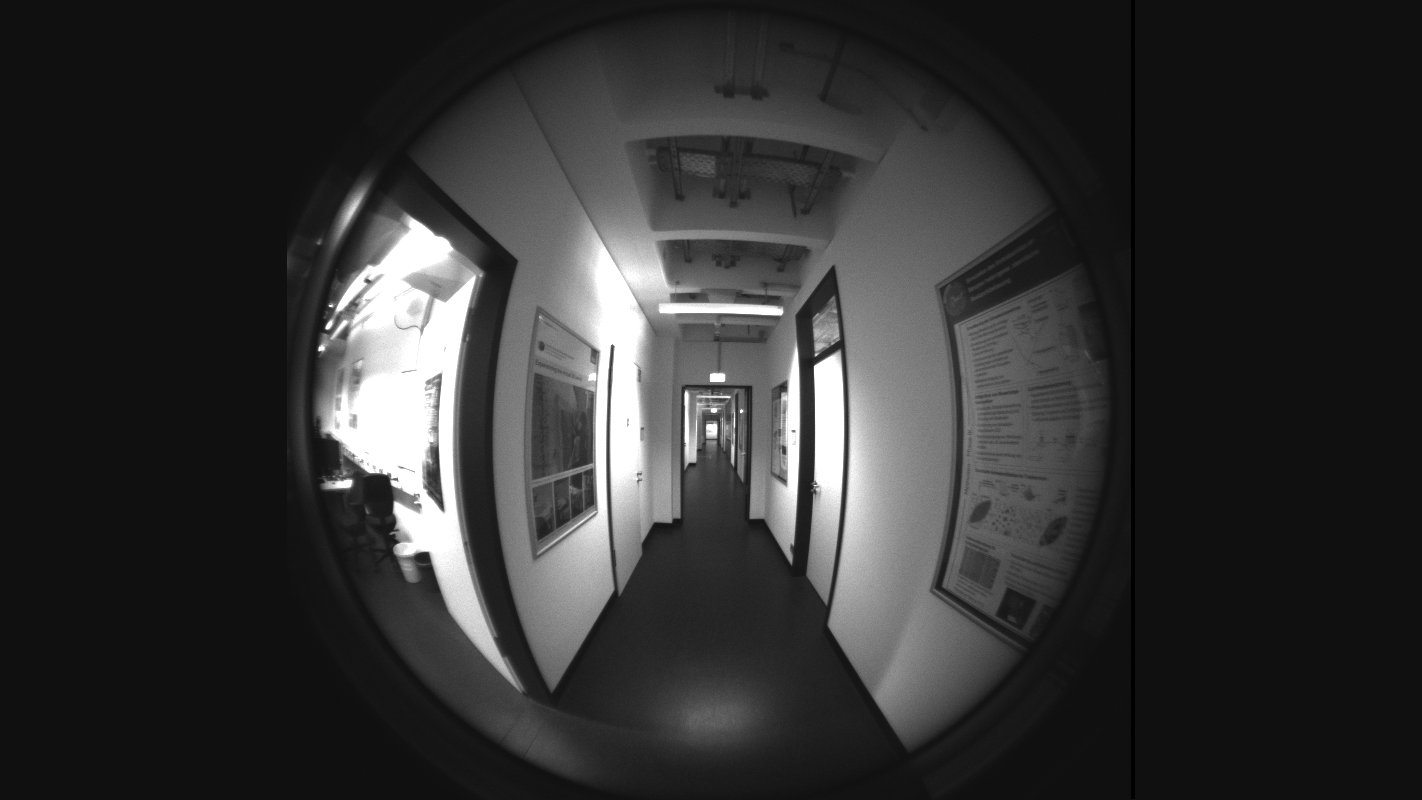
\includegraphics[width=\linewidth]{images/real_dataset/f2_frame000005.png}
		\caption{Fischaugenkamera 2 \\ (T265)}
		\label{subfig:fisheye2}
	\end{subfigure}
	\hfill \medskip
	\begin{subfigure}[t]{0.3\linewidth}
		\centering
		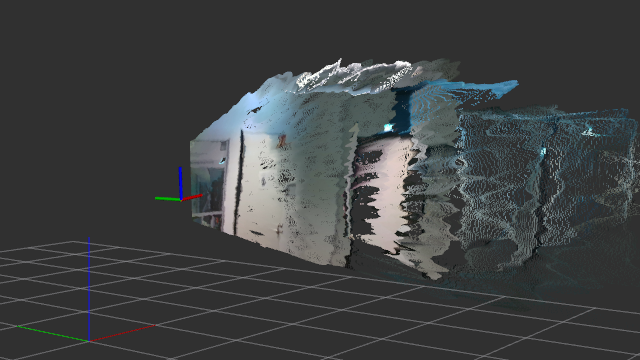
\includegraphics[width=\linewidth]{images/real_dataset/pointcloud1.png}
		\caption{Pose (T265) + \\ 3D Punktwolke (D435)}
		\label{subfig:odom2}
	\end{subfigure}
	\hfill
	\begin{subfigure}[t]{0.3\linewidth}
		\centering
		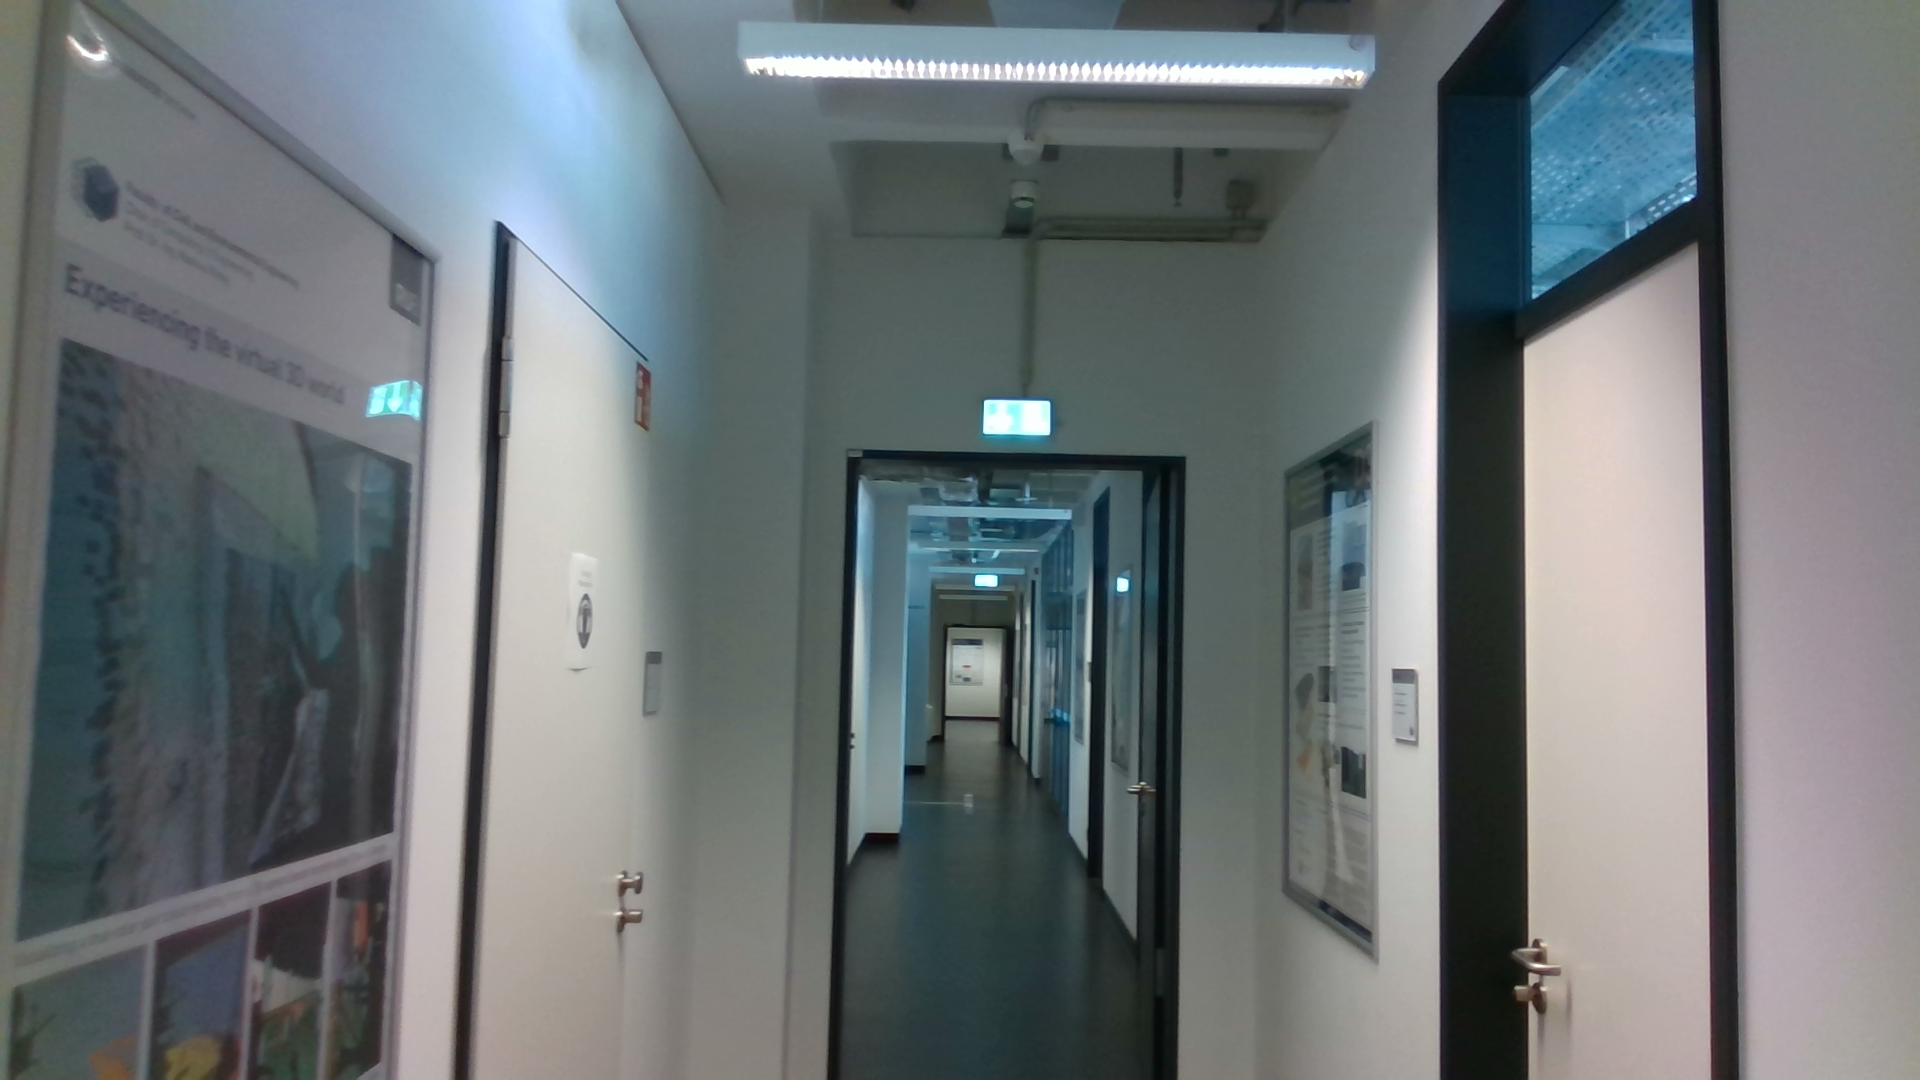
\includegraphics[width=\linewidth]{images/real_dataset/dc_frame000005.png}
		\caption{RGB-Bild \\ (D435) \hspace*{2cm}}
		\label{subfig:rgb-image}
	\end{subfigure}
	\hfill
	\begin{subfigure}[t]{0.3\linewidth}
		\centering
		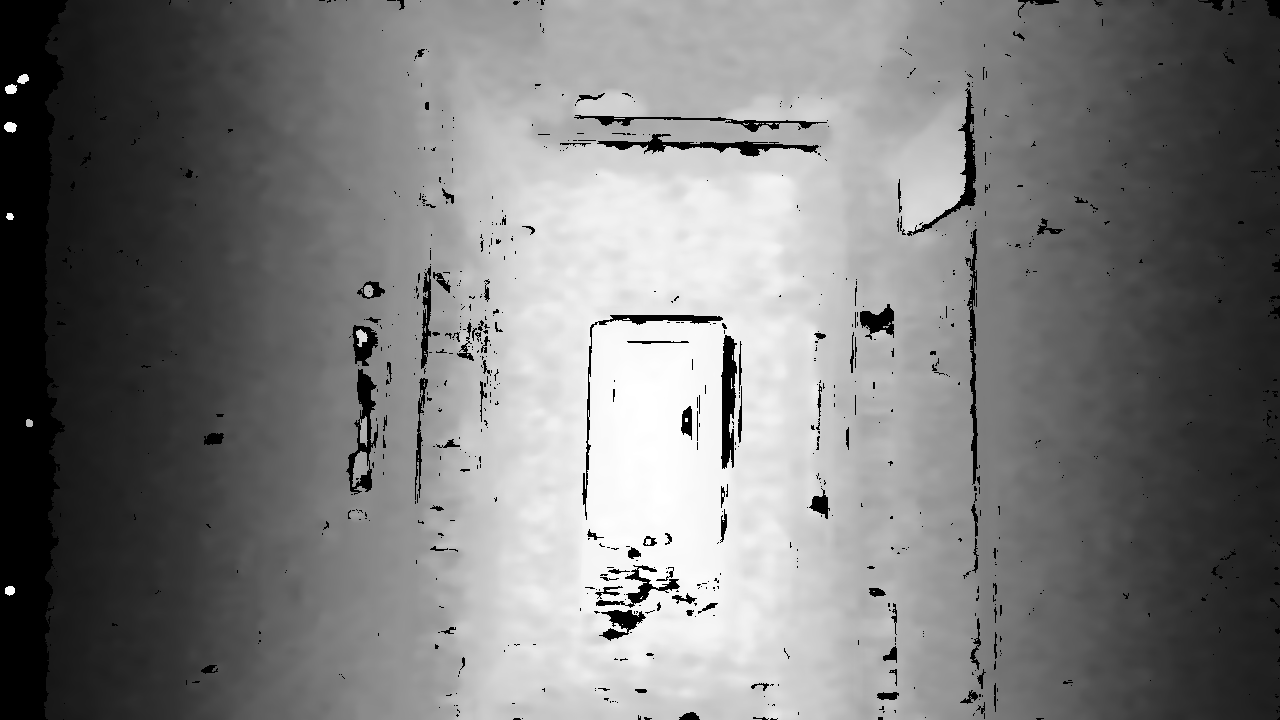
\includegraphics[width=\linewidth]{images/real_dataset/dt_frame000005.png}
		\caption{Tiefenbild \\ (D435) \hspace*{2cm}}
		\label{subfig:depth-image}
	\end{subfigure}
	\caption{Datensatz pro Frame. \subref{subfig:odom1} und \subref{subfig:odom2} visualisieren in unterschiedlichen Perspektiven die von der T265 ermittelte Odometrie und die von der D435 erhaltenen 3D Punktwolke. \subref{subfig:fisheye1} und \subref{subfig:fisheye2} sind die von der T265 aufgenommenen Fischaugenbilder. \subref{subfig:rgb-image} ist das RGB-Bild der D435 und \subref{subfig:depth-image} das dazugehörige Tiefenbild. }
	\label{fig:dataset}
\end{figure}

\subsection{Generierung der synthetischen Daten}
\label{subsec:generate_synth_images}
Für die Generierung der synthetischen Daten wurden die 3D-Gebäudemodelle aus dem BIM der Gebäuden entnommen. Die 3D-Gebäudemodelle wurden in Blender\footnote{\url{https://www.blender.org/about/} (aufgerufen am: 20.07.2019)} in der derzeitig aktuellen Version 2.79b simuliert. Die Strecken der realen Aufnahmen wurden in den Simulationen Konsistenz halber auf einer konstanten Höhe von 1.70$m$ bestmöglich schwankungslos imitiert. Eine exakte Imitation der Aufnahmestrecke der realen Daten war wegen des Abdriftens der von der T265 berechneten Ground-Truth-Daten nicht möglich (s. Abschn. \ref{subsec:record_real_data}).

Um die Varianz der realen Daten abzudecken, wurde in Anlehnung an \citet{acharyaBIMPoseNetIndoorCamera2019} entlang der imitierten Strecke in 0.05$m$ Intervallen und mit einer $\pm$10° Neigung in je y- und z-Achse Bilder mit korrespondierenden Ground-Truth-Daten aufgenommen. Die intrinsischen Daten der D435 RGB-Kamera wurden auf die virtuellen Kameras übertragen. Aus Gründen der Performance wurde die Auflösung der synthetischen Bilder von $1920\times1080$ auf $960\times540$ halbiert. Abbildung \ref{fig:dataset_variation} illustriert die Variationen der Pose pro Stützpunkt auf einer Strecke.


\begin{figure}
	\centering
	\begin{subfigure}[t]{0.18\linewidth}
		\centering
		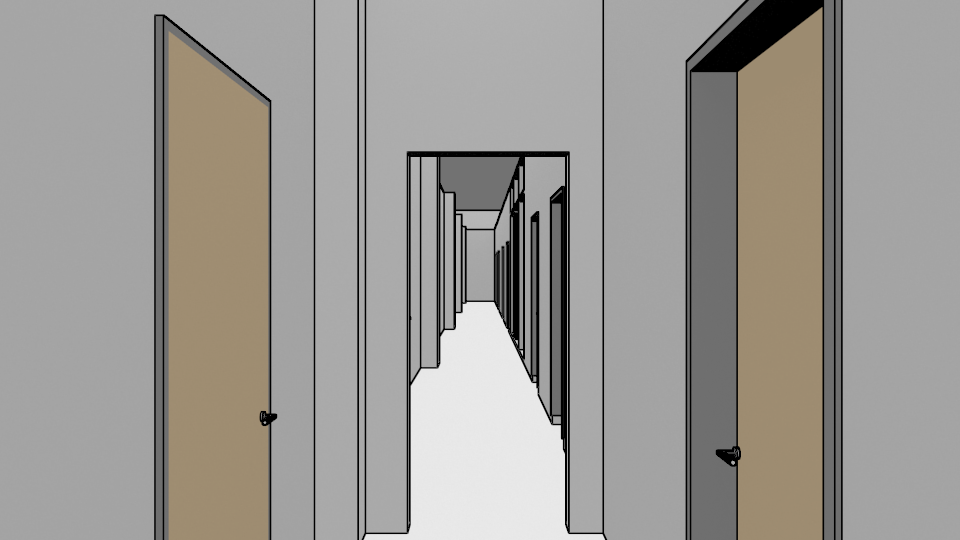
\includegraphics[width=\linewidth]{images/syn_dataset/00023.png}
		\caption{Orginal Pose \vspace{\fill}}
		\label{subfig:iz0_y0}
	\end{subfigure}
	\hfill 
	\begin{subfigure}[t]{0.18\linewidth}
		\centering
		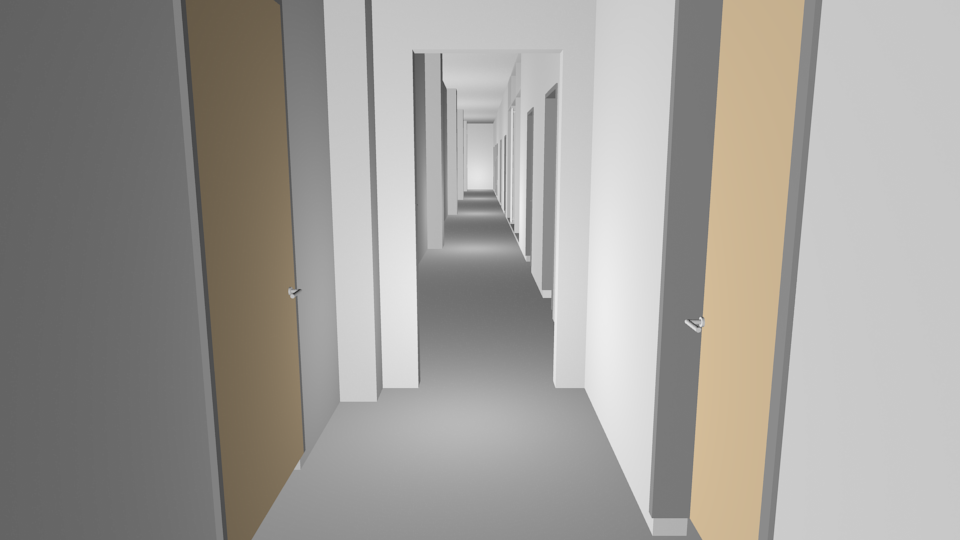
\includegraphics[width=\linewidth]{images/syn_dataset/00021.png}
		\caption{-10° um die y-Achse}
		\label{subfig:iz0_y-10}
	\end{subfigure}
	\hfill
	\begin{subfigure}[t]{0.18\linewidth}
		\centering
		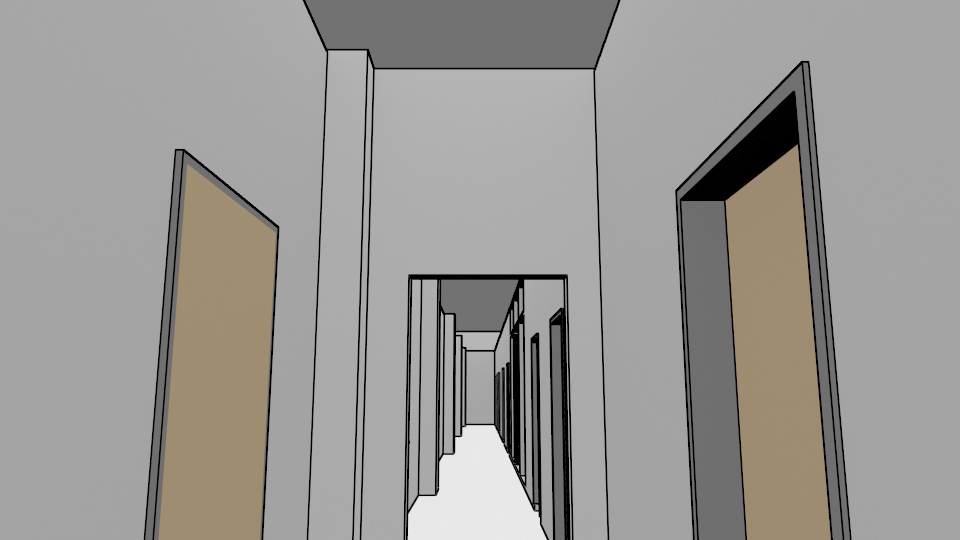
\includegraphics[width=\linewidth]{images/syn_dataset/00020.png}
		\caption{+10° um die y-Achse}
		\label{subfig:iz0_y+10}
	\end{subfigure}
	\hfill
	\begin{subfigure}[t]{0.18\linewidth}
		\centering
		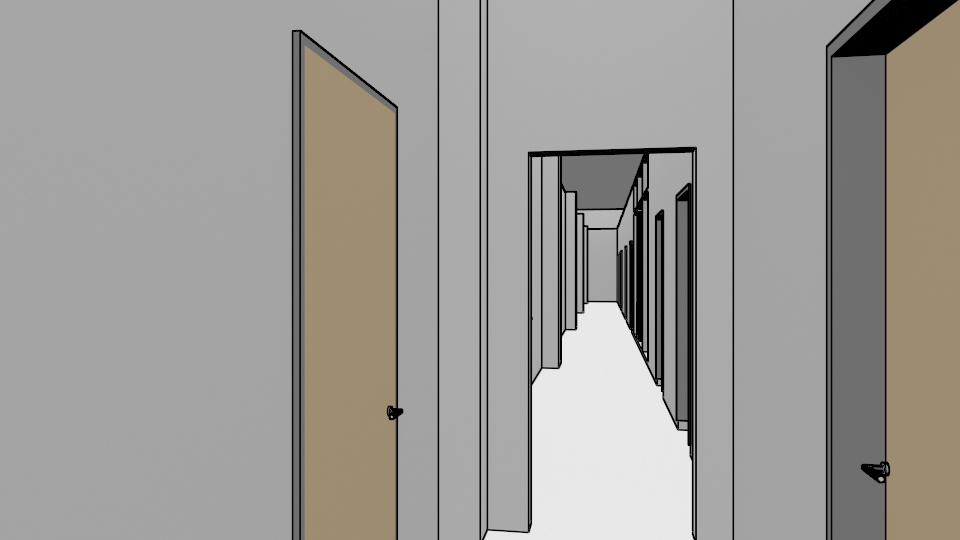
\includegraphics[width=\linewidth]{images/syn_dataset/00024.png}
		\caption{-10° um die z-Achse}
		\label{subfig:iz-10_y0}
	\end{subfigure}
	\hfill
	\begin{subfigure}[t]{0.18\linewidth}
		\centering
		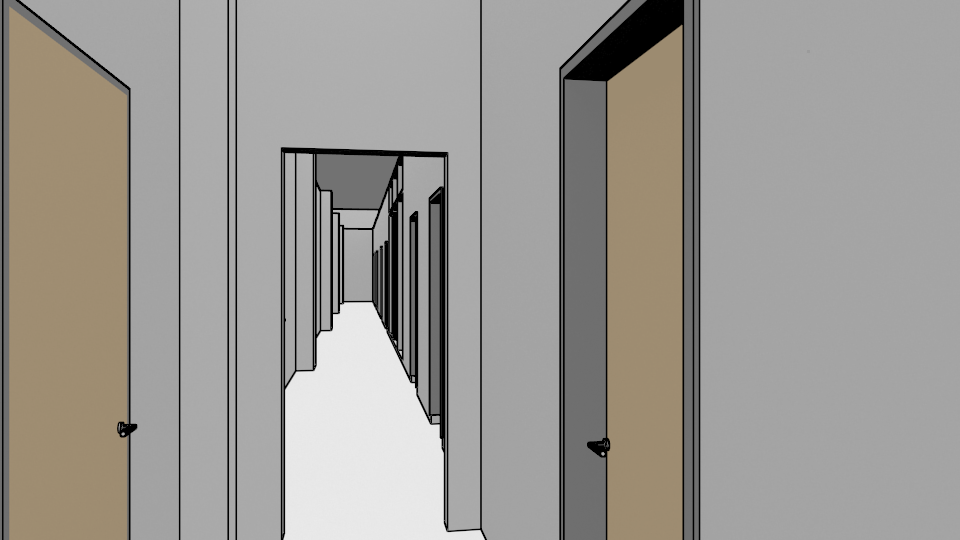
\includegraphics[width=\linewidth]{images/syn_dataset/00022.png}
		\caption{+10° um die z-Achse}
		\label{subfig:iz+10_y0}
	\end{subfigure}
	\caption{Variation der Pose pro Stützpunkt auf einer Strecke.}
	\label{fig:dataset_variation}
\end{figure}

Insgesamt wurden gleicherweise wie die synthetischen Datensätze von \citet{acharyaBIMPoseNetIndoorCamera2019} drei synthetische Datensätze pro Strecke erzeugt, die sich in der Beschaffenheit von karikaturistische Darstellung (\textit{cartoon}), zu synthetischen Kantenbilder (\textit{edge}) hin über zu fotorealistische Darstellung (\textit{photoreal}) unterscheiden (s. Abb. \ref{fig:dataset_preprocess}). Bei der Generierung der Datensätze \textit{cartoon} und \textit{photoreal} wurde die Beleuchtung aus einem Netz von Punktlichtquellen nachgestellt, um die Lichteffekte der echten Lampen realitätsnäher zu simulieren. Weiterhin wurde für die Erzeugung der Datensätze von \textit{edge} wurden die Kanten der 3D-Objekte über Blender markant sichtbar konfiguriert und eine homogene Beleuchtung verschaffen, damit die Kanten hervorstechen und unberührt von Beleuchtungseffekte bleiben (s. Abb. \ref{fig:dataset}). 

Die Datensätze \textit{cartoon} und \textit{photoreal} unterscheiden sich ausschließlich in den Render-Engines. Blender 2.79b verfügt die Render-Engines \textit{Blender-Internal} und \textit{Blender-Cycles}. Während die Blender-Internal Engine beim Rendern die Berechnung der Lichtstrahlen abkürzt, versucht die Blender-Cycles Engine über \textit{Raytracing}-Algorithmen das Verhalten des Lichtes mit ihren physikalischen Eigenschaften realistischer zu simulieren. Daher wurden die Datensätze \textit{cartoon} sowie \textit{edge} über die Render-Engine \textit{Blender-Internal} und der Datensatz \textit{photoreal} über die \textit{Blender-Cycles} Engine generiert.

\subsection{Verarbeitung der Daten}
Die vorliegende Arbeit versucht das PoseNet Modell mit den Gradientenbildern der synthetischen Daten zu trainieren und mit den Gradietenbildern der realen Daten zu evaluiert. Demzufolge wurde nach der Erhebung der realen Bilder und Generierung der synthetischen Bilder diese in ihre Gradientenbilder verarbeitet. 

Bei der Aufnahme der realen Daten kam es durch die manuelle Führung des Kamerakonstrukts (s. Abb. \ref{fig:t265_d435}) in den Gebäuden zu unscharfen Bildern. Im Vergleich zu unscharfen Kanten im Bild weisen schärfere Kanten eine deutlichere Kontur im Gradientenbild auf. Daher wurden die realen Bilder vor der Verarbeitung in Gradientenbilder auf die Größe $960 \times 540$ der synthetischen Bilder verkleinert. Hiermit sollen einerseits eine einheitliche Auflösung der Bilder verschafft und andererseits durch Bewegung bedingte unscharfe Kanten im Bild zu einer schärferen Kante zusammengeführt werden.

Die künstliche Beleuchtung in den Gebäudesimulationen führte bei den Gradientenbildern der karikaturistischen Daten (\textit{grad-cartoon}) zu Artefakten (s. Abb. \ref
{fig:treshold}). Diese Artefakte befanden sich im niedrigen Wertebereich des Gradientenbildes. Deshalb wurde für die Unterdrückung der Artefakte zusätzlich ein Schwellenwertverfahren angewendet, indem die Pixelwerte eines Gradientenbildes unter einer gewissen Schwelle auf ein Mindestwert gesetzt wurden. Nach einem Minimum der Pixelwerte wurde iterativ gesucht, sodass die von den Artefakten betroffenen Stellen eine homogene Fläche im Bild darstellten. Der Wert 8 stellte sich als geeignete Schwelle für die Gradientenbilder heraus und wurde als Minimum für die Pixelwerte festgelegt, sodass die Pixelwerte der Gradientenbilder im Wertebereich von $[8,255]$ lagen. Da es sich bei dem Pixelwert 8 um einen kleinen Wert handelte, wurde dieses Verfahren Konsistenz halber bei allen Datensatztypen angewendet. Abbildung \ref{fig:dataset_preprocess} visualisiert von jedem Datensatztyp ein Beispiel und die dazugehörigen Gradientenbilder.


\begin{figure}
	\centering
	\begin{tikzpicture}[zoomboxarray, 
	connect zoomboxes,
	zoomboxarray columns=2,
	zoomboxarray rows=1,
	zoombox paths/.append style={thick, orange},
	figurename=notresh]
	\node [image node] { 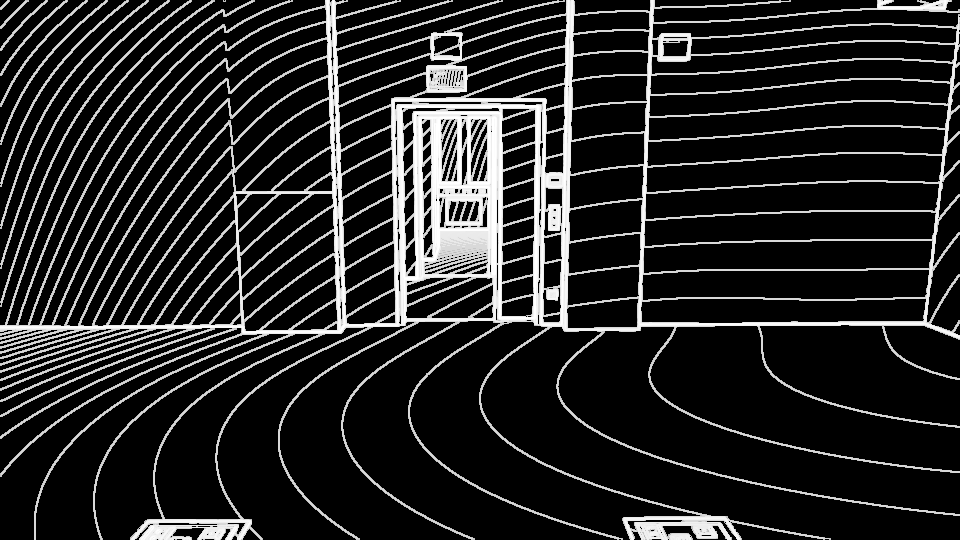
\includegraphics[width=0.24\textwidth]{images/treshold/0_tresh_binared.png} };
	\zoombox[magnification=10]{0.15,0.8}
	\zoombox[magnification=10]{0.5,0.25}
	\end{tikzpicture}
	\begin{tikzpicture}[zoomboxarray, 
	connect zoomboxes,
	zoomboxarray columns=2,
	zoomboxarray rows=1,
	zoombox paths/.append style={thick, orange},
	figurename=treshed]
	\node [image node] { 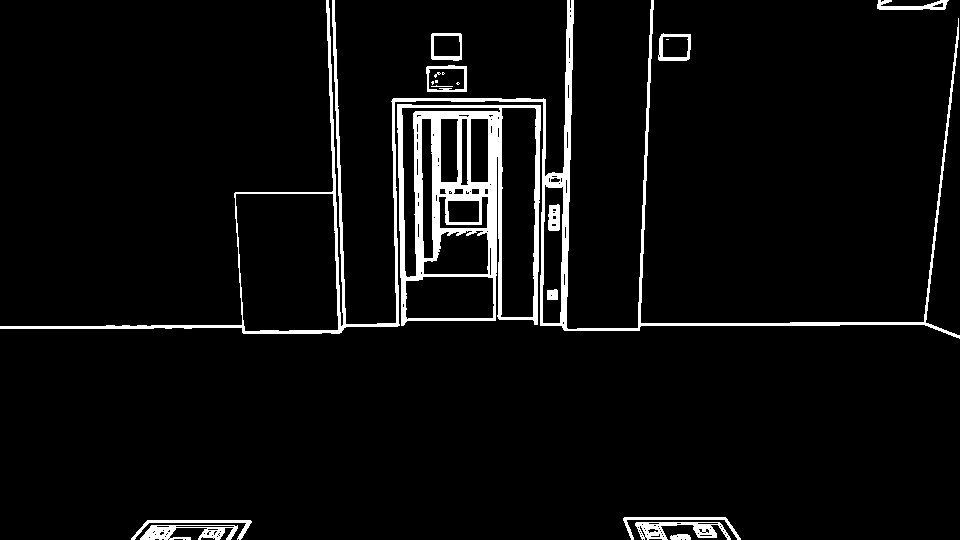
\includegraphics[width=0.24\textwidth]{images/treshold/8_tresh_binared.png} };
	\zoombox[magnification=10]{0.15,0.8}
	\zoombox[magnification=10]{0.5,0.25}
	\end{tikzpicture}
	\caption{Darstellung der durch die künstliche Beleuchtung entstehenden Artefakten in den \textit{grad-cartoon} Daten. Für eine bessere Visualisierung der Artefakte wurden die Gradientenbilder binarisiert. \subref{notresh-image} ist ein Gradientenbild ohne Anwendung eines Schwellenwertverfahrens; \subref{treshed-image} ist ein Gradientenbild mit Anwendung eines Schwellenwertverfahrens.}
	\label{fig:treshold}
\end{figure}


\begin{figure}
	\centering
	\begin{subfigure}[t]{0.24\linewidth}
		\centering
		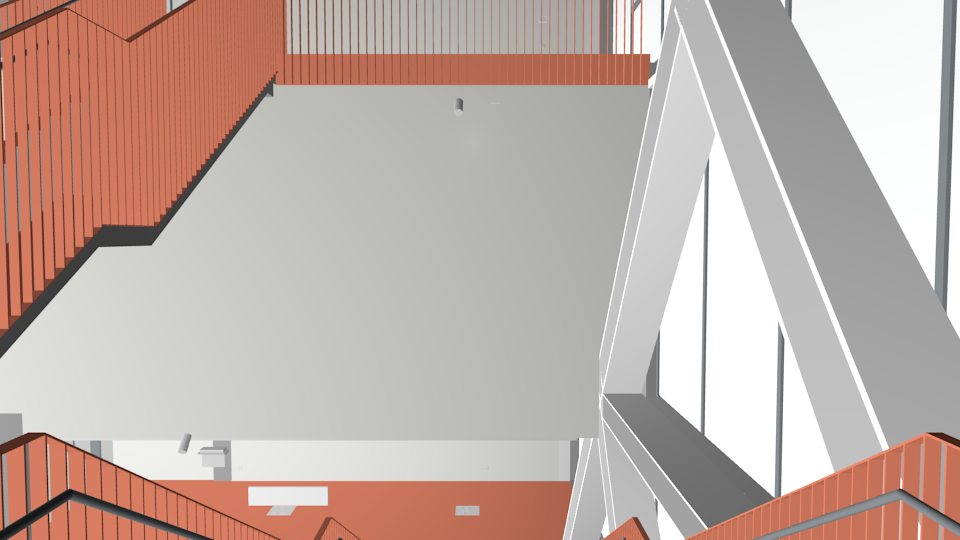
\includegraphics[width=\linewidth]{images/syn_dataset/b00188.png}
		\caption{\RaggedRight karikaturistische Simulation \hspace{2cm} (\textit{cartoon})}
		\label{subfig:cartoonish}
	\end{subfigure}
	\hfill
	\begin{subfigure}[t]{0.24\linewidth}
		\centering
		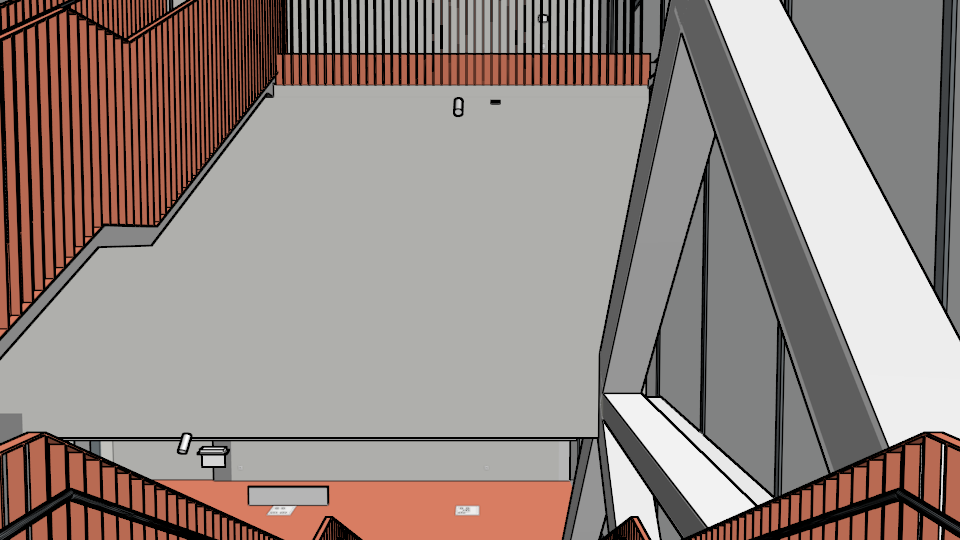
\includegraphics[width=\linewidth]{images/syn_dataset/e00188.png}
		\caption{\RaggedRight synthetisches Kantenbild \hspace{2cm} (\textit{edge})}
		\label{subfig:edge}
	\end{subfigure}
	\hfill
	\begin{subfigure}[t]{0.24\linewidth}
		\centering
		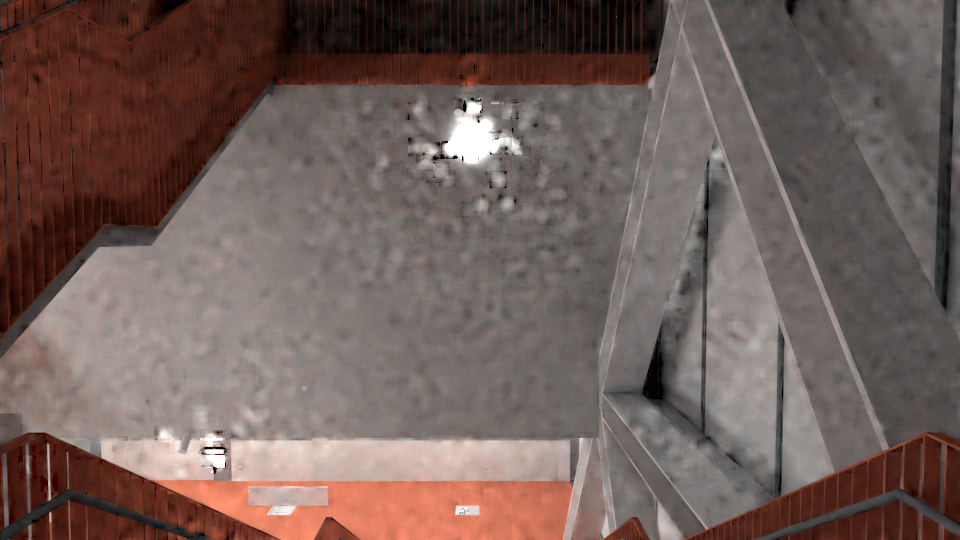
\includegraphics[width=\linewidth]{images/syn_dataset/c00188.png}
		\caption{\RaggedRight fotorealistische Simulation \hspace{2cm} (\textit{photoreal})}
		\label{subfig:photorealistic}
	\end{subfigure}
	\hfill 
	\begin{subfigure}[t]{0.24\linewidth}
		\centering
		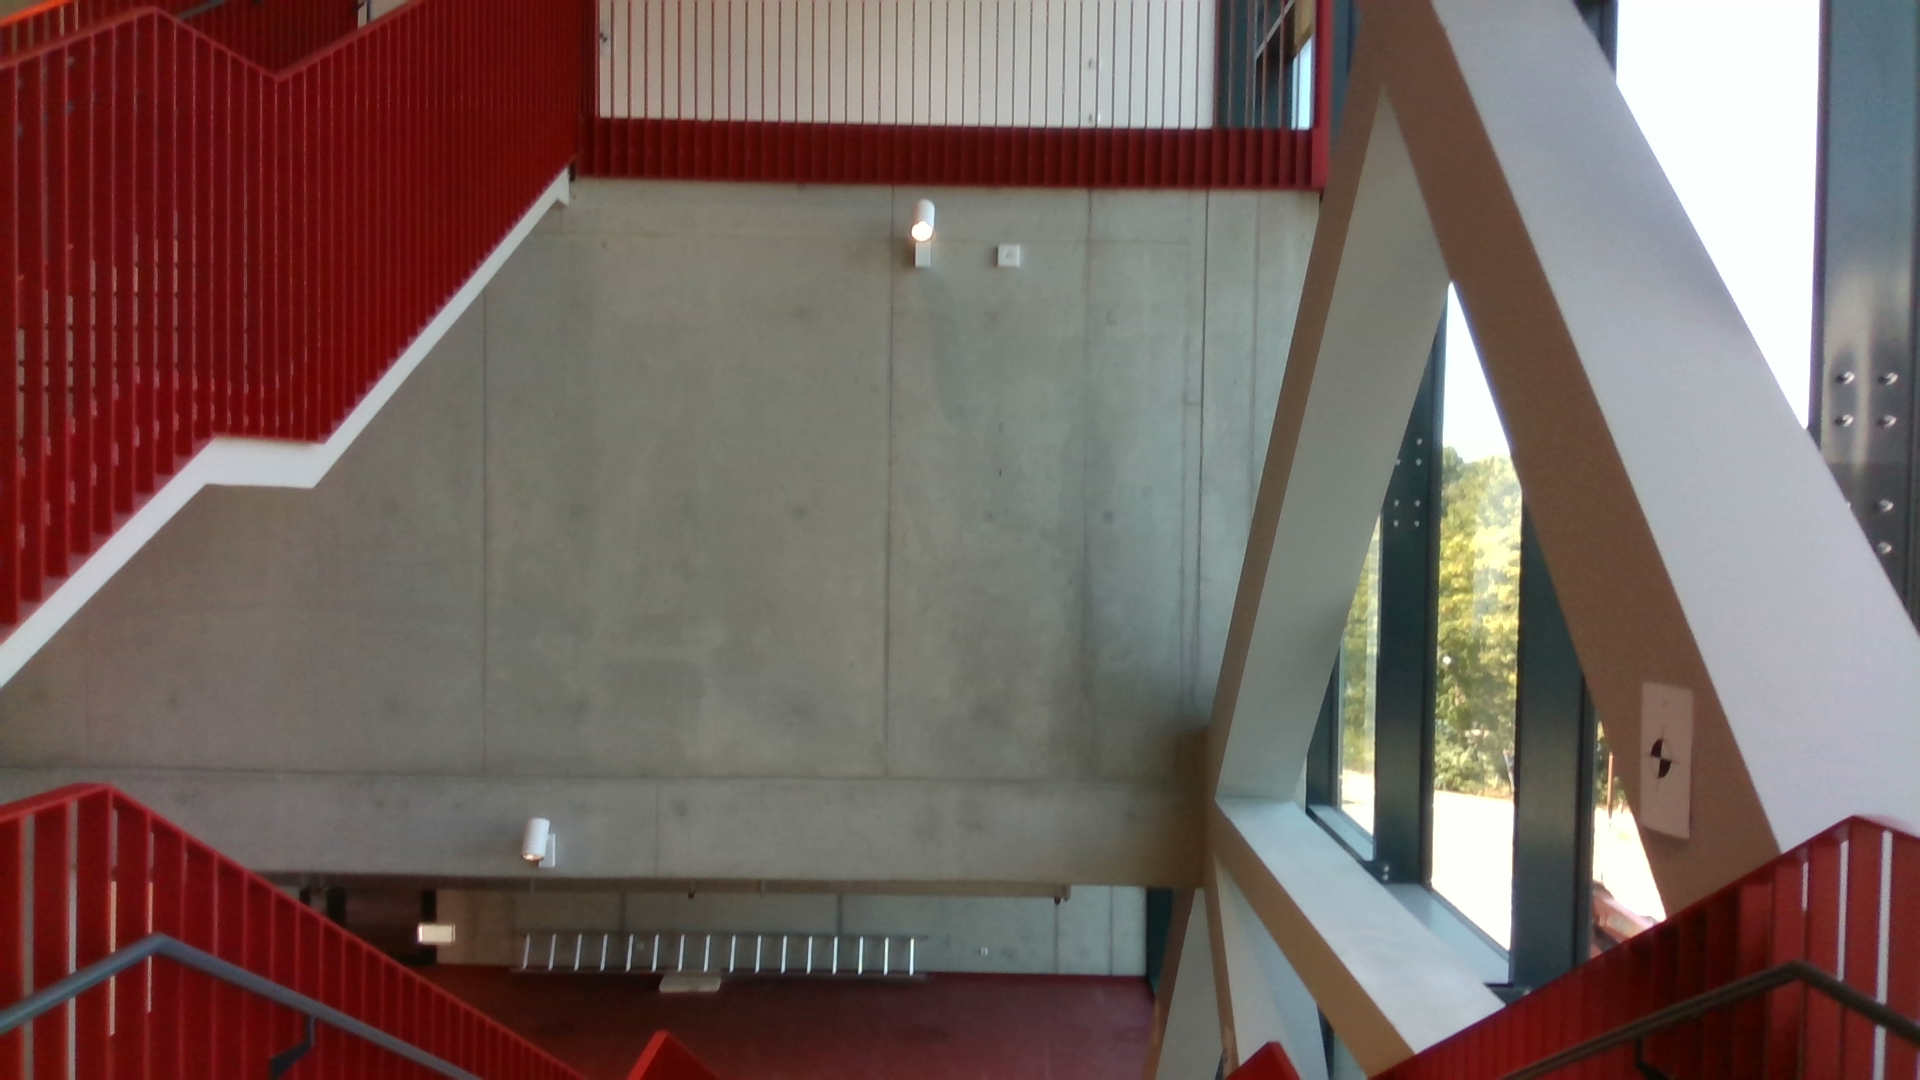
\includegraphics[width=\linewidth]{images/syn_dataset/r000089.png}
		\caption{\RaggedRight{reale Aufnahme} \hspace{2cm} (\textit{real})}
		\label{subfig:real}
	\end{subfigure}
	\hfill 
	\begin{subfigure}[t]{0.24\linewidth}
		\centering
		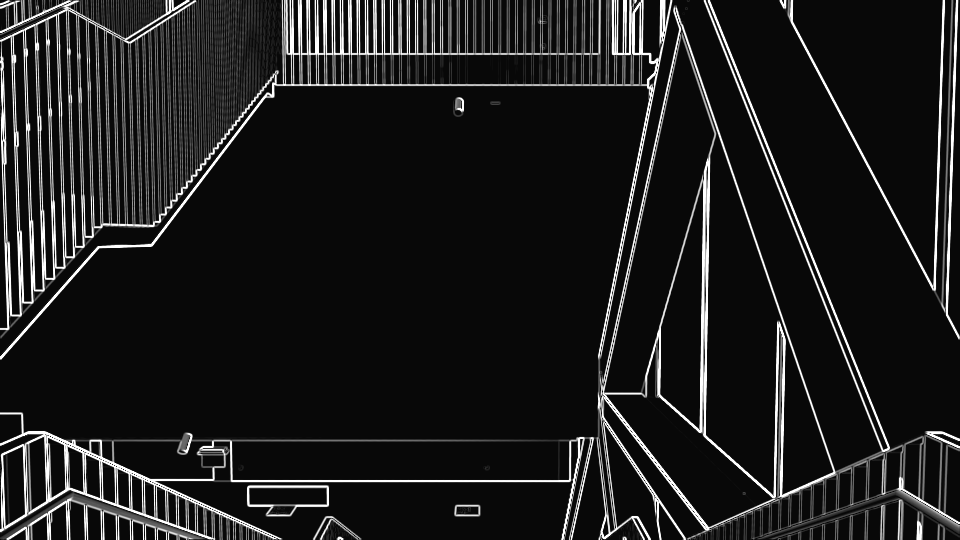
\includegraphics[width=\linewidth]{images/syn_dataset/bg00188.png}
		\caption{\RaggedRight{Gradientenbild von \subref{subfig:cartoonish} \hspace{2cm} (\textit{grad-cartoon})}}
	\end{subfigure}
	\hfill
	\begin{subfigure}[t]{0.24\linewidth}
		\centering
		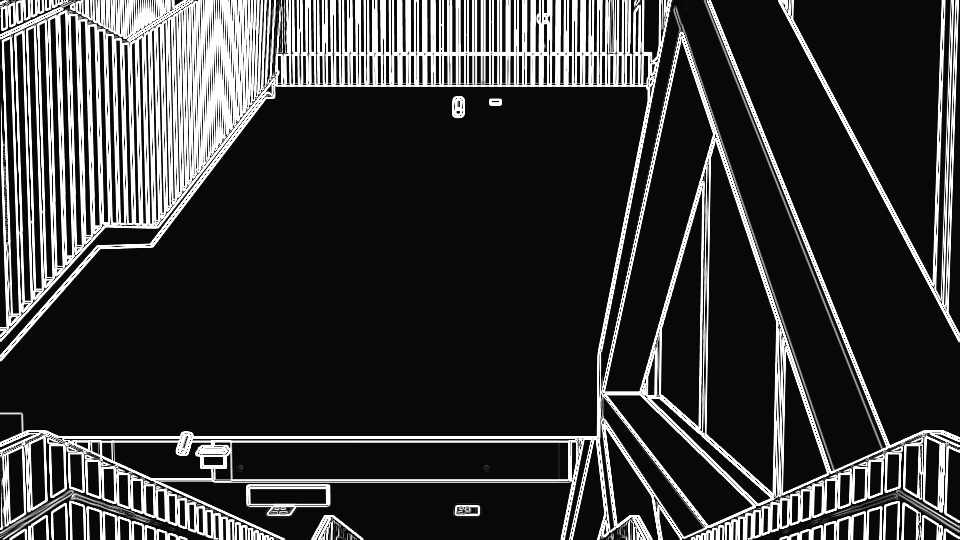
\includegraphics[width=\linewidth]{images/syn_dataset/eg00188.png}
		\caption{\RaggedRight{Gradientenbild von \subref{subfig:edge} \hspace{2cm} (\textit{grad-edge})}}
	\end{subfigure}
	\hfill
	\begin{subfigure}[t]{0.24\linewidth}
		\centering
		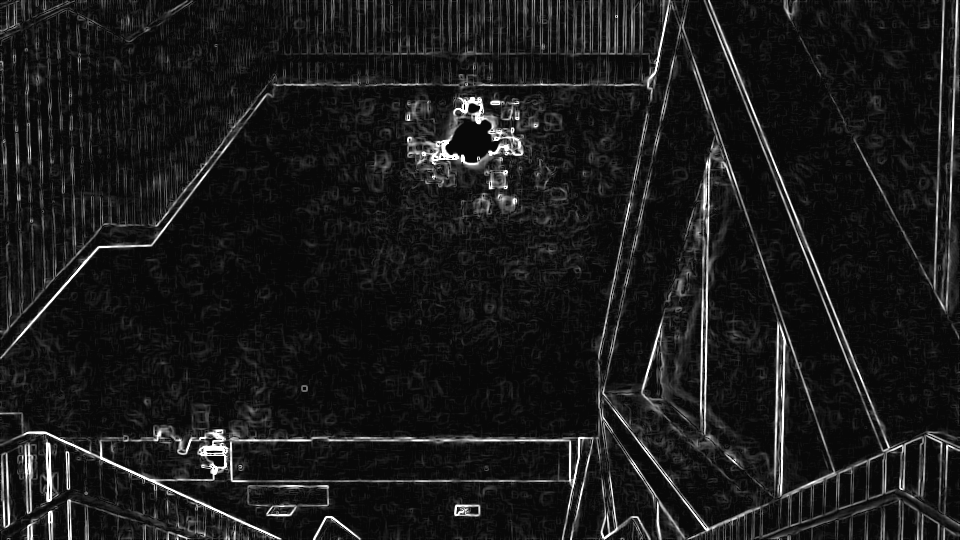
\includegraphics[width=\linewidth]{images/syn_dataset/cg00188.png}
		\caption{\RaggedRight{Gradientenbild von \subref{subfig:photorealistic} \hspace{2cm} (\textit{grad-photoreal})}}
	\end{subfigure}
	\hfill
	\begin{subfigure}[t]{0.24\linewidth}
		\centering
		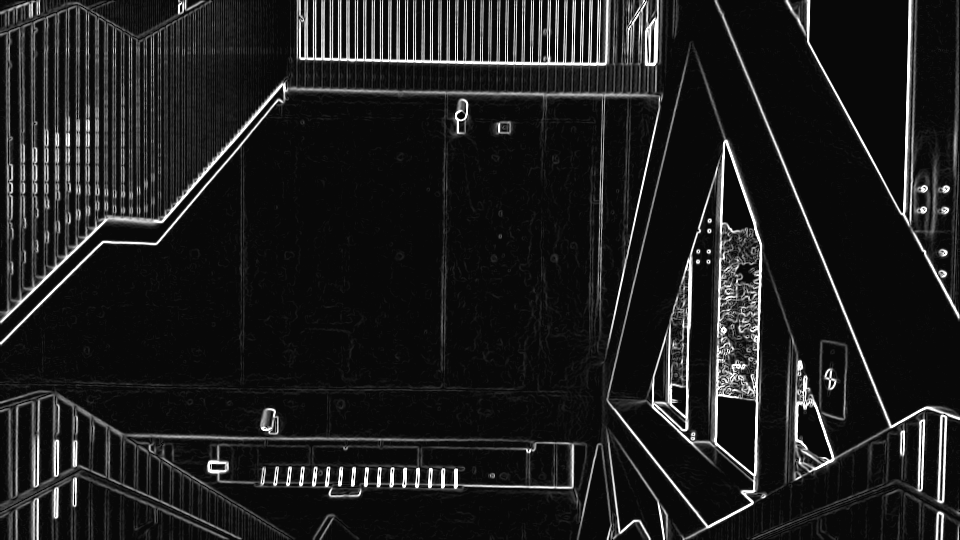
\includegraphics[width=\linewidth]{images/syn_dataset/rg000089.png}
		\caption{\RaggedRight{Gradientenbild von \subref{subfig:real} \hspace{2cm} (\textit{grad-real})}}
	\end{subfigure}
	\hfill
	\caption{Beispielhafte Bilder für jeden Datensatztyp und die dazu korrespondierenden Gradientenbildern. Die Daten sind aus dem \textit{HS-stairs-down} Datensatz.}
	\label{fig:dataset_preprocess}
\end{figure}

\cleardoublepage



\subsection{Datensätze}
\label{subsec:datasets}
Diese Arbeit versucht den Ansatz von \citet{acharyaBIMPoseNetIndoorCamera2019} in größeren Gebäudesimulation und auf längeren Strecken zu untersuchen. Der Datensatz von \citet{acharyaBIMPoseNetIndoorCamera2019} erstreckt sich über ca. 18$m$ in einem ca. $20m \times 5m$ großen Korridor auf einer Etagenebene. Die Aufnahme verlief überwiegen in einer Richtung (s. Abb. \ref{fig:acharya_traj}). Daher wurden für die Erzeugung der Datensätze längere Aufnahmestrecken festgelegt, die einerseits in mehrere Richtungen verliefen und andererseits sich auf mehreren Etagenebenen erstreckten. 

\begin{figure}
	\centering
	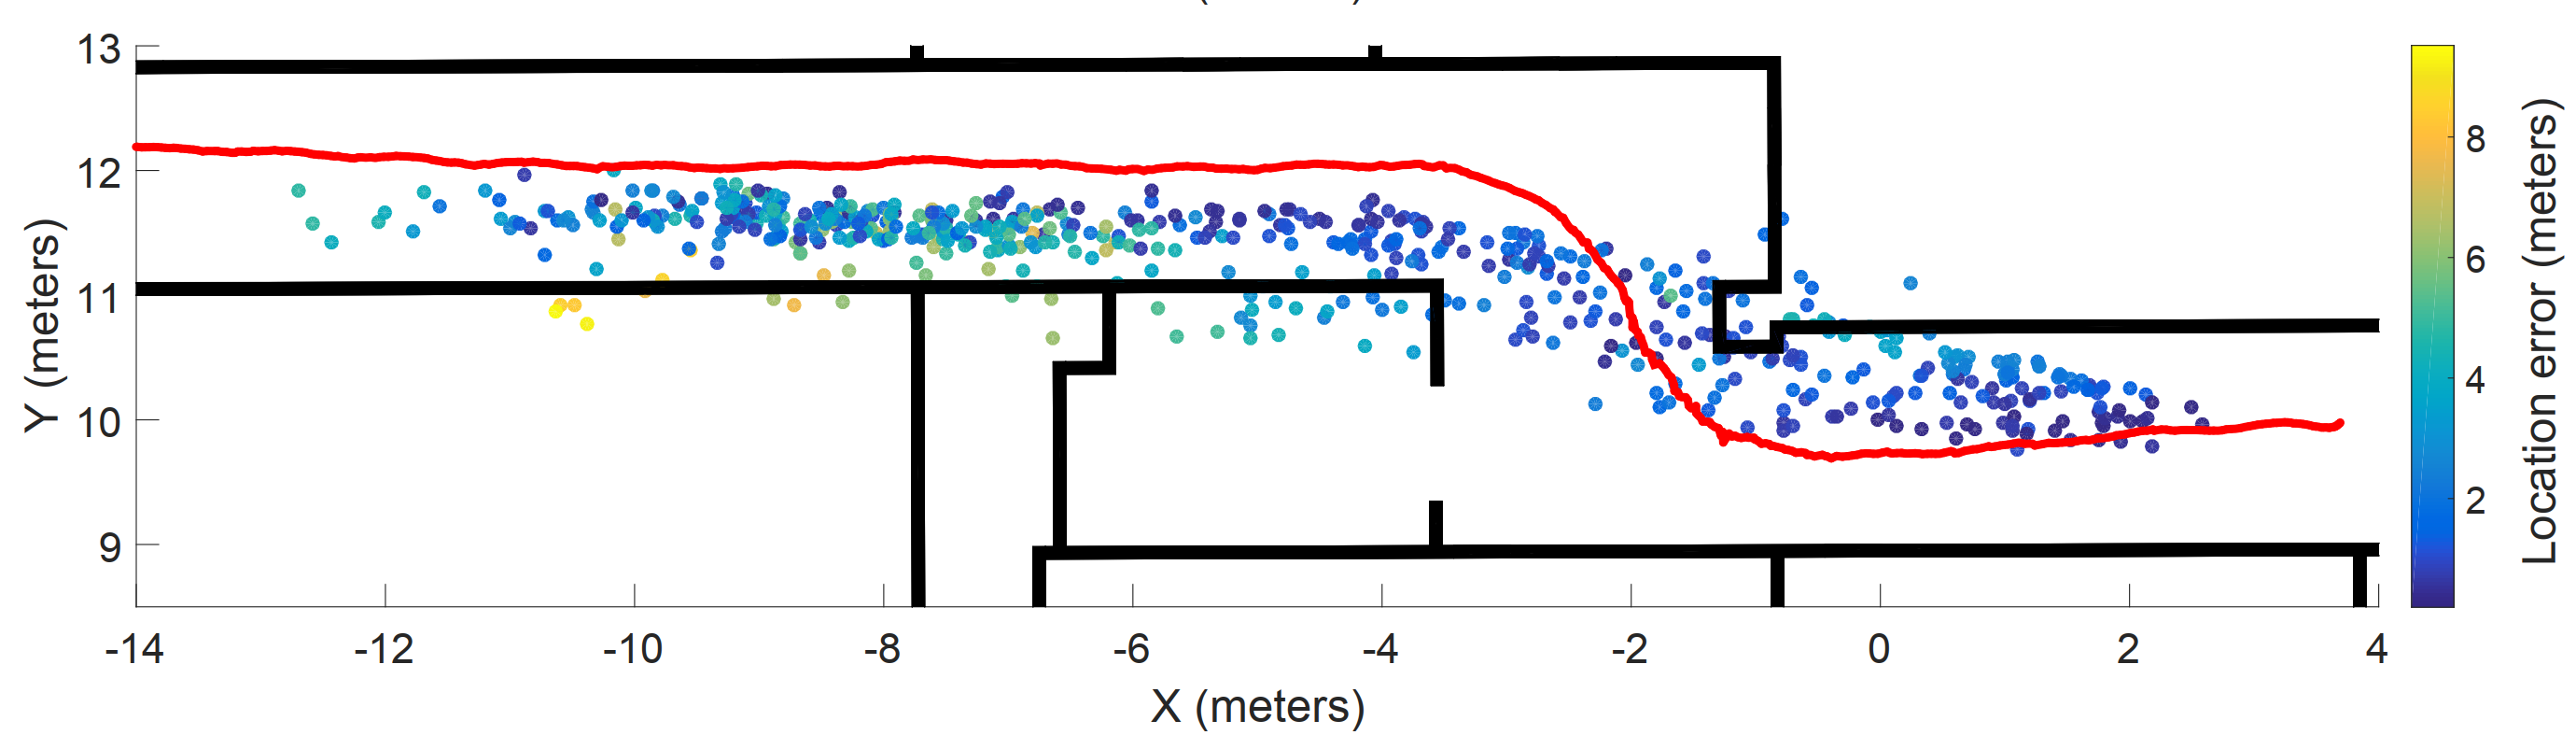
\includegraphics[width=1.0\textwidth]{images/trajectories/acharya_traj.png}
	\caption{Darstellung des Lokalisierungsergebnisses von \citet{acharyaBIMPoseNetIndoorCamera2019}, die durch das Trainieren mit den synthetischen Kantenbildern und der anschließenden Evaluierung mit den Gradientenbildern der realen Daten resultierte. Die Aufnahmestrecke der realen Daten ist in Rot dargestellt. Die Aufnahme auf der Strecke verlief von rechts nach links. Entnommen aus \cite{acharyaBIMPoseNetIndoorCamera2019}.}
	\label{fig:acharya_traj}
\end{figure}




In dieser Arbeit wurden Daten aus der nördlichen Hälfte des 6. Stockwerkes des IC-Gebäudes der Ruhr-Universität Bochum (IC) und aus dem Seminargebäude der Hochschule Bochum (HS) erhoben bzw. synthetische Daten aus den Gebäudesimulationen generiert. Die Gebäude unterschieden sich im Detail der Simulationen (s. Abb. \ref{fig:difference_3d}). Die Simulation vom IC enthielt wiederholende Gebäudemerkmale und sehr wenige Objekte. Deshalb wurde im IC nur ein Datensatz erhoben, der eine geschlossene Schleife in einem Flur bildete. Im Gegensatz dazu enthält die Simulation vom HS ein Treppenhaus mit eindeutigen Merkmalen sowie mehr Objekte wie z.B. die Objekte der technischen Gebäudeausrüstung. Demzufolge wurden drei Datensätze im HS erhoben, die einerseits in mehreren Richtungen auf einer ebenen Strecke verliefen und anderseits sich über mehrere Etagenebenen im Treppenhauses erstreckten.




Die  als \textit{IC-loop} bezeichnete ca. $115m$ lange Strecke im ersten Datensatz bildete eine geschlossene Schleife in einem $50m \times 11m \times 3.5m$ Bereich des ICs. Die $65m$ lange Strecke im \textit{HS-gamma} Datensatz einhielt in der Mitte eine Schleife und überging zu einem optisch ähnlichen Flur wie der Ausgangsflur in einem Bereich von ca. $54m \times 10m \times 3m$ des HS-Gebäudes. Im Datensatz \textit{HS-stairs-up} wurde eine Treppe im HS aufwärts bestiegen und im Datensatz \textit{HS-stairs-down} dieselbe Treppe abgestiegen. Die Strecken auf den Treppen waren ca. $32m$ lang und befanden sich in einer ca. $12m \times 12m \times 12m$ Teilzone vom HS.
Tabelle \ref{tab:dataset_metrics} listet die approximierten metrischen Eigenschaften der Datensätze auf. 
Die variierende Länge der Strecken führte bei den realen sowie synthetischen Datensätze zu Mengenunterschiede. Tabelle \ref{tab:datasets} stellt die Datenmenge der Datensätzen dar.
Abbildung \ref{fig:trajectories} illustriert die Strecken der Datensätze. 
\begin{figure}
	\centering
	\begin{subfigure}[t]{0.48\linewidth}
		\centering
		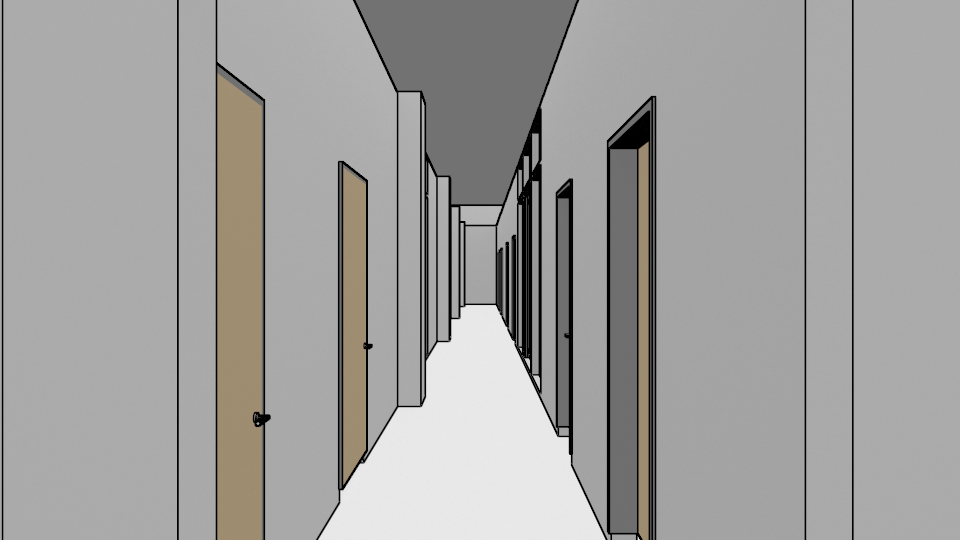
\includegraphics[width=\linewidth]{images/syn_dataset/ic00343.png}
		\caption{IC Simulation}
		\label{subfig:ic_syn_example}
	\end{subfigure}
	\hfill
	\begin{subfigure}[t]{0.48\linewidth}
		\centering
		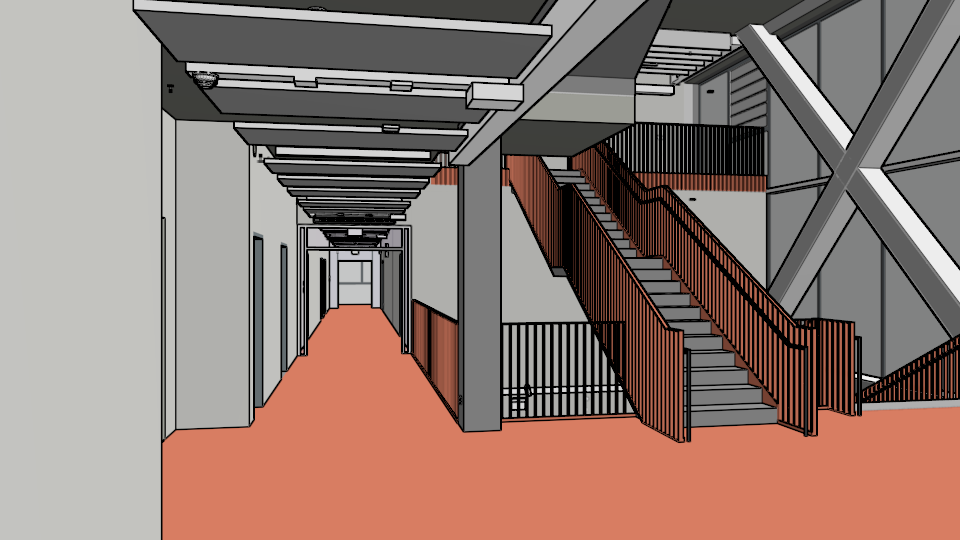
\includegraphics[width=\linewidth]{images/syn_dataset/hs_gamma02162.png}
		\caption{HS Simulation}
		\label{subfig:hs_gamma_syn_example}
	\end{subfigure}
	\caption{Veranschaulichung der Gebäudesimulationen. Für eine bessere Visualisierung sind die Kanten markant dargestellt. Während die Wände, die Decke und der Boden in \subref{subfig:ic_syn_example} wenig Detail beinhalten, sind diese in \subref{subfig:hs_gamma_syn_example} detailreicher mit technischen Gebäudeausrüstungen wie z.B. Steckdose ausgestattet.}
	\label{fig:difference_3d}
\end{figure} 

\begin{table}
	\centering
	\caption{Approximierte metrische Eigenschaften der Datensätze.}
	\begin{tabularx}{1.0\textwidth}{X X X >{\arraybackslash}p{1.7cm} }
		\textbf{Bezeichnung} & \textbf{Streckenlänge} & \textbf{Volumen} & \textbf{Gebäude}\\
		\hline
		IC-loop & $115m$ & $50m \times 11m \times 3.5m$ & IC \\
		\hline
		HS-gamma & $65m$ & $54m \times 10m \times 3m$ & HS\\
		\hline
		HS-stairs-up & $32m$ & $12m \times 12m \times 12m$ & HS\\
		\hline
		HS-stairs-down & $32m$ & $12m \times 12m \times 12m$ & HS\\
	\end{tabularx}
	\label{tab:dataset_metrics}
\end{table}


\begin{table}
	\centering
	\caption{Datenmenge der Datensätze.}
	\begin{tabularx}{1.0\textwidth}{p{3.5cm} X >{\arraybackslash}p{1.7cm} }
		\textbf{Bezeichnung} & \textbf{Anzahl reale Daten} (synthetische Daten) & \textbf{Gebäude}\\
		\hline
		IC-loop & 3842 (11435) & IC\\
		\hline
		HS-gamma & 1958 (6490) & HS\\
		\hline
		HS-stairs-up & 1068 (3160)& HS\\
		\hline
		HS-stairs-down & 1161 (3245) & HS\\
	\end{tabularx}
	\label{tab:datasets}
\end{table}


\begin{figure}
	\centering
	\begin{subfigure}[t]{1.0\linewidth}
		\centering
		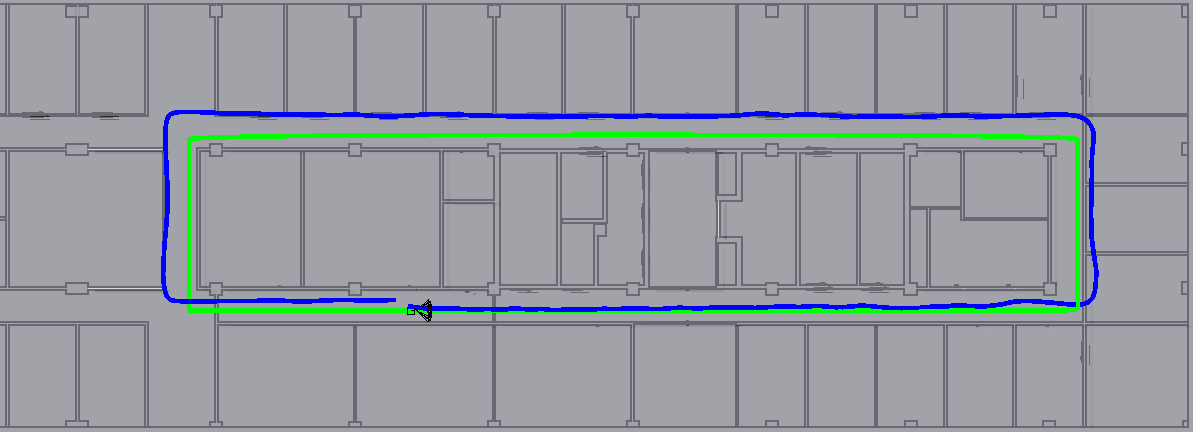
\includegraphics[width=\linewidth]{images/trajectories/ic_traj.png}
		\caption{\textit{IC-loop}}
		\label{subfig:traj_ic}
	\end{subfigure}
	\hfill \medskip
	\begin{subfigure}[t]{1.0\linewidth}
		\centering
		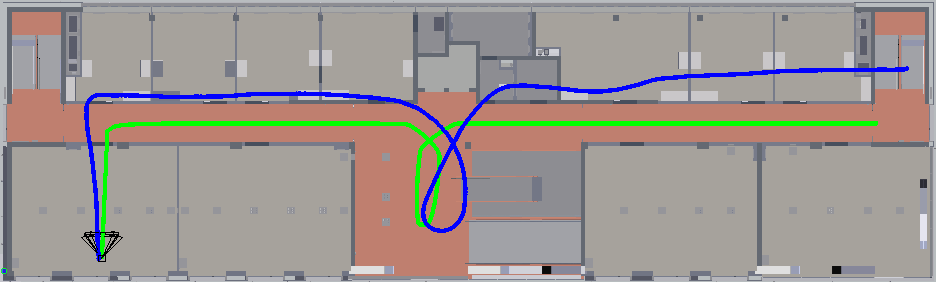
\includegraphics[width=\linewidth]{images/trajectories/hs_gamma.png}
		\caption{\textit{HS-gamma}}
		\label{subfig:traj_hs_gamma}
	\end{subfigure}
	\hfill \medskip
	\begin{subfigure}[tr]{0.45\linewidth}
		\flushleft
		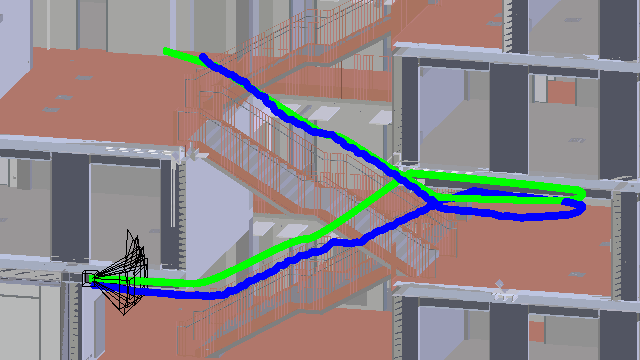
\includegraphics[width=\linewidth]{images/trajectories/hs_up.png}
		\caption{\textit{HS-stairs-up}}
		\label{subfig:traj_hs-up}
	\end{subfigure}
	\hfill
	\begin{subfigure}[tl]{0.45\linewidth}
		\flushright		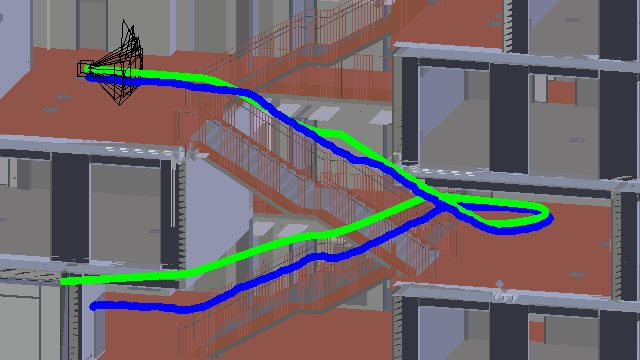
\includegraphics[width=\linewidth]{images/trajectories/hs_down.png}
		\caption{\textit{HS-stairs-down}}
		\label{subfig:traj_hs-down}
	\end{subfigure}
	\hfill
	\caption{Illustration der Aufnahmestrecken der Datensätze. Die Aufnahmestrecken der synthetischen Daten werden in Grün und die von der T265 mit einer Abweichung bis zur 5\% berechneten Strecke der realen Daten in Blau gekennzeichnet. Die schwarzen Umrisse der virtuellen Kameras geben den Ausganspunkt sowie die Aufnahmerichtung der Strecken an. \subref{subfig:traj_ic} befindet sich in der nördlichen Hälfte des 6. Stockwerkes des IC-Gebäudes der Ruhr-Universität Bochum. \subref{subfig:traj_hs_gamma}, \subref{subfig:traj_hs-up}, \subref{subfig:traj_hs-down} befinden sich im Seminargebäude der Hochschule Bochum. \subref{subfig:traj_hs-up} und \subref{subfig:traj_hs-down} sind nahe an der Position der Schleife von \subref{subfig:traj_hs_gamma}.}
	\label{fig:trajectories}
\end{figure}

\subsection{Trainingsparameter}
Künstlichen neuronalen Netzwerke besitzen zwei Arten von Parametern. Die erste Art von Parametern (\textit{Gewichte}) werden während der Trainingsphase über Verfahren wie z.B. \textit{Backpropagation} an die Trainingsdaten angepasst.
Die zweite Art von Parametern (\textit{Hyperparameter}) werden vor der Trainingsphase festgelegt und geben besondere Einstellungen des Netzwerkes wie z.B. das Lernverhalten an. Die Performance eines KNNs ist abhängig von seinen Parametern \cite{goodfellowDeepLearning2016}. Da diese Arbeit den Ansatz von \citet{acharyaBIMPoseNetIndoorCamera2019} in größeren Gebäudesimulation und auf längeren Strecken zu untersuchen versuchte, wurde die Performance des KNNs bestmöglich von den verwendeten Datensätzen abhängig gehalten. Dazu wurden die Hyperparametern von \citet{acharyaBIMPoseNetIndoorCamera2019} übernommen bzw. gleichermaßen bestimmt oder im selben Verhältnis zum Datensatz gewählt.

% Hyperparameter können über Grid-Search Verfahren optimiert werden, indem die Akkuratesse der Netzwerke mit variierenden Hyperparametern paarweise verglichen werden


In der vorliegenden Arbeit wurde für das Training der Netzwerke die Caffe \cite{jiaCaffeConvolutionalArchitecture2014} Implementierung von PoseNet verwendet, die von den eigenen Autoren \citet{kendallPoseNetConvolutionalNetwork2015} veröffentlicht wurde. Die Batchgröße betrug 40 und die Anzahl der Trainingsepochen war 160. Eine NVIDIA GeForce GTX 1080 Ti mit 11GB Grafikspeicher wurde verwendet und ermöglichte bei einer Batchgröße von 40 drei Trainingsprozesse zeitgleich durchzuführen.

Jeder reale sowie synthetische Datensatz (s. Tab. \ref{tab:datasets}) wurde je in 50\% Trainings- und 50\% Evaluationsdaten zufällig aufgeteilt und auf eine Auflösung von $480\times270$ skaliert. Während des Trainingsprozesses wurden zufällige Ausschnitte der Größe $224 \times 224$ aus dem skalierten Trainingsdatensatz genommen. Für die Evaluierung wurde ein zentrierter Ausschnitt derselben Größe aus dem skalierten Evaluationsdatensatz verwendet. Das Durchschnittsbild der Trainingsdaten wurde sowohl beim Trainieren als auch bei der Evaluierung von den Inputbildern subtrahiert. 

Der Hyperparameter $\beta$ der von PoseNet vorgestellten Kostenfunktion (s. Gleichung \ref{eq:posenet_loss}) wurde wie empfohlen für jeden realen Datensatz durch ein \textit{Grid-Search}-Verfahren bestimmt. Dazu wurde mit den realen Trainingsdaten trainiert und mit den realen Evaluationsdaten evaluiert. Der \textit{Loss} wurde mit dem \textit{AdaGrad} \cite{duchiAdaptiveSubgradientMethods2011} Gradientenabstiegsverfahren mit einer konstanten Lernrate von $10^{-3}$ optimiert bzw. minimiert. Vorab wurden die Gewichte des Netzwerks mit den Gewichten eines Modells initialisiert, das zuvor auf der GoogLeNet Architektur mit dem Places Datensatz trainiert wurde. Tabelle \ref{tab:trainingparams} gibt eine Übersicht der Hyperparameter an.

\cleardoublepage
\begin{table}[bp]
	\centering
	\caption{Übersicht der Hyperparameter.}
	\begin{tabularx}{1.0\textwidth}{X X}
		\textbf{Hyperparameter} & \textbf{Wert}\\
		\hline
		Architektur & PoseNet (s. Abschn. \ref{sec:posenet})\\
		\hline
		Implementierung & Caffe \\
		\hline
		Batchgröße & $40$\\
		\hline
		Anzahl der Epochen & $160$\\
		\hline
		Datenaufteilung & \makecell[tl]{
			50\% Trainingsdaten\\
			50\% Evaluationsdaten\\
		}\\
		\hline
		Bildskalierung & $480 \times 270$\\
		\hline
		Bildausschnitt& \makecell[tl]{
			$224 \times 244$\\
			(\textit{Training}: zufällig, \textit{Evaluation}: zentriert)\\
		}\\
		\hline
		Datensatznormierung & Subtraktion des Durchschnittsbildes der Trainingsdaten \\
		\hline
		\makecell[tl]{
			$\beta$ der Kostenfunktion\\
			(s. Gleichung \ref{eq:posenet_loss}) 
		} &
		\makecell[tl]{
			\textit{IC-loop}: 680\\
			\textit{HS-gamma}: 120\\
			\textit{HS-stairs-up}: 470\\
			\textit{HS-stairs-down}: 610\\
		}\\
		\hline
		Loss-Optimierer & AdaGrad\\
		\hline
		Lernrate & $10^{-3}$\\
		\hline
		Initialisierung der Gewichte & Gewichte eines mit dem Places Datensatz trainierten Modells auf GoogLeNet \\
	\end{tabularx}
	\label{tab:trainingparams}
\end{table}
\cleardoublepage
% !TEX root = ../my_thesis.tex

\section{Ergebnisse}
Im vorliegenden Kapitel werden die Ergebnisse der durchgeführten Experimente präsentiert. In dieser Arbeit gibt ein Evaluationsergebnis eines Netzwerkes die Abweichung der Position in Metern sowie Orientierung in Grad an und der Median der Evaluationsergebnisse bestimmt die Akkuratesse eines KNNs. Somit bildet sich die Akkuratesse eines Netzwerkes aus der Zusammensetzung von Positions- sowie Orientierungsfehler. In dieser Arbeit wird ein Evaluationsergebnis und eine Akkuratesse gegenüber Seinesgleichen anhand des Positionsfehlers verglichen.

Im weiteren Verlauf dieses Kapitels werden zuerst die Reproduktionsergebnisse von BIM-PoseNet \cite{acharyaBIMPoseNetIndoorCamera2019} angegeben. Anschließend werden die Evaluationsergebnisse der trainierten Netzwerke angezeigt.

\subsection{Reproduktion der Ergebnisse von BIM-PoseNet}
Die Ergebnisse der Experimente von \citet{acharyaBIMPoseNetIndoorCamera2019}, die das PoseNet Model mit Gradientenbilder der karikaturistischen Daten (\textit{grad-cartoon}) sowie synthetischen Kantenbilder trainierten (\textit{grad-edge}) und anschließend mit den Gradientenbildern der realen Daten (\textit{grad-real}) evaluierten, konnten näherungsweise (vgl. Tab. \ref{tab:reproduction}) reproduziert werden. Abweichend von BIM-PoseNet wurden statt 1000 reale Bilder, 600 reale Bilder evaluiert, weil zu derzeit 600 Evaluierungsbilder veröffentlicht waren. Der Trainingsprozess wurde pro Datensatztyp 5-mal wiederholt und die bessere Akkuratesse wurde behalten. Eine exakte oder bessere Reproduktion der Ergebnisse ist durch Zufall bedingt und wurde in dieser Arbeit aus Zeitgründen vernachlässigt. Tabelle \ref{tab:reproduction} präsentiert die Ergebnisse der Reproduktion sowie die Ergebnisse der Autoren \citet{acharyaBIMPoseNetIndoorCamera2019}.


\begin{table}[b]
	\centering
	\caption{Reproduktionsergebnisse. Abweichungen der Ergebnisse sind durch Zufall bedingt und können bei mehrfachem Wiederholen des Trainingsprozesses minimiert bzw. erhoben sowie verbessert werden. }
	\begin{tabularx}{1.0\textwidth}{X X X}
		\textbf{Trainingsdatensatz} \hspace{2cm} (Gradientenbild) & \textbf{BIM-PoseNet} \hspace{2cm} (Position, Orientierung) & \textbf{Reproduktion} \hspace{2cm} (Position, Orientierung)\\
		\hline
	 \textit{grad-cartoon} & 2.63$m$, 6.99° & 2.57$m$, 10.52°\\
		\hline
		\textit{grad-edge} & 1.88$m$, 7.73°  & 2.53$m$, 9.54°\\
	\end{tabularx}
	\label{tab:reproduction}
\end{table}





\subsection{Evaluation der trainierten KNNs}
Für alle synthetischen Datensätze wurde separat das Trainingsprozess 5-mal mit den korrespondierenden Gradientenbildern der Trainingsdaten wiederholt. Eine Evaluierung folgte mit den Gradientenbildern der korrespondierenden synthetischen und realen Evaluationsdaten. Es wurden pro Strecke (s. Tab. \ref{tab:dataset_metrics}) und Datensatztyp nur die beste Akkuratesse behalten. Tabelle \ref{tab:results_ic} bis \ref{tab:results_hs_stairs_down} geben die Akkuratesse der KNNs auf den jeweiligen Strecken an. 

Für ein besseres Verständnis der durch die Evaluierung mit den \textit{grad-real} Datensätzen resultierenden Akkuratessen wurden für die KNNs mit der besten Akkuratesse pro Strecke die bestimmten Positionen in der xy-Ebene dargestellt. Ebenso wurden pro Strecke der Positionsfehler in der xy-Ebene und der Orientierungsfehler auf der Gierachse der jeweiligen Evaluationsdaten dargestellt. Abbildungen \ref{fig:result_ic_loop} bis \ref{fig:result_hs_stairs_down} illustrieren die Evaluationsergebnisse.


\subsubsection{IC-loop}
% die eine geschlossen Schleife in einem optisch ähnlichen Flur bildet,
%  der Ansatz von \citet{acharyaBIMPoseNetIndoorCamera2019} auf einer ebenen, gegen den UZS abwechselnde Richtung verlaufenden, ca. 115$m$ langen Strecke mit wiederholenden Gebäudemerkmalen 
% Alle Datensätze der Strecke \textit{IC-loop} wurden zu 50\% Trainingsdaten und zu 50\% Evaluierungsdaten zufällig aufgeteilt. Für alle synthetischen Datensatztypen mit je 5718 Daten wurde ein separates Netzwerk trainiert. Anschließend wurden die Netzwerke mit den korrespondierenden synthetischen Evaluierungsdatensätze mit je 5717 Daten getestet. Eine weitere Evaluierung der trainierten Netzwerke folgte mit den realen 1921 Evaluierungsdaten. Tabelle \ref{tab:results_ic} gibt die Ergebnisse dieser Evaluierungsvorgänge an.
% Aus Tabelle \ref{tab:results_ic} ist zu erkennen,

In diesem Experiment wurde der \textit{IC-loop} Datensatz verwendet. 
Ausschließlich mit synthetischen Daten beim Trainieren und Evaluieren konnte eine Akkuratesse von 1.61$m$ in der Position und 8.17° in der Orientierung durch den \textit{grad-cartoon} Datensatz erzielt werden (vgl. Tab. \ref{tab:results_ic}). Dies zeigt die potenzielle Fähigkeit des Experimentes zur Pose Estimation auf der \textit{IC-loop} Strecke bei Daten derselben Domäne. 

Bei der Evaluierung mit den Gradientenbildern der realen Evaluationsdaten konnte auf dem mit \textit{grad-photoreal} trainiertem Netzwerk eine Akkuratesse von 16.68$m$ in der Position und 73.25° in der Orientierung erreicht werden (vgl. Tab. \ref{tab:results_ic}). Bei einem Gebäudevolumen von ca. $50m \times 11m \times 3.5m$ ist die Positionsgenauigkeit von 16.68$m$, mit Anbetracht des Abdriftens der realen Ground-Truth-Daten (s. Abschn. \ref{subsec:record_real_data}), für ein denkbares Lokalisierungsverfahren zu ungenau. Genauso ist eine Orientierungsgenauigkeit von 73.25° für die Bestimmung der Orientierung mehr als ungeeignet. Abbildung \ref{fig:result_ic_loop} visualisiert die Evaluierungsergebnisse von dem mit \textit{grad-photoreal} trainiertem sowie mit \textit{grad-real} evaluiertem Netzwerk.

In Abbildung \ref{subfig:ic_fig2} ist deutlich zu erkennen, dass das mit \textit{grad-photoreal} trainierte Netzwerk die Positionen aller \textit{grad-real} Evaluationsdaten verteilt auf einem ca. 30$m$ langen Teilbereich der unteren horizontalen Strecke bestimmt hat. Daher weisen Evaluationsdaten der kürzeren vertikalen sowie der obigen horizontalen Strecke die größten Positionsfehler auf (vgl. Abb. \ref{subfig:ic_fig4}). Ebenso kommt in Abbildung \ref{subfig:ic_fig6} hervor, dass das Netzwerk größtenteils die Orientierung der Evaluationsdaten als die Aufnahmerichtung der unteren horizontalen Strecke bestimmt hat.

\begin{table}
	\centering
	\caption{Evaluationsergebnisse von der Strecke \textit{IC-loop}. Es wird die Akkuratesse der mit den jeweiligen Trainingsdaten trainierten Netzwerke angegeben, die mit den korrespondierenden synthetischen Evaluationsdaten sowie jeweils mit den realen Evaluationsdaten evaluiert wurden.  }
	\begin{tabularx}{1.0\textwidth}{X >{\RaggedRight}X >{\RaggedRight}X}
	\textbf{Trainingsdatensatz} \hspace{2cm} (Gradientenbild) & \textbf{synthetische Daten} \hspace{2cm} (Position, Orientierung) & \textbf{reale Daten} \hspace{2cm} (Position, Orientierung)\\
	\hline
		\textit{grad-cartoon} & 1.61$m$, 8.17° & 23.56$m$, 51.30°\\
		\hline
		\textit{grad-edge} & 2.00$m$, 8.29° & 32.91$m$, 59.17°\\
\hline
		\textit{grad-photoreal} & 1.80$m$, 7.70° & 16.68$m$, 73.25°\\
	\end{tabularx}
	\label{tab:results_ic}
\end{table}



\begin{figure}
	\setlength\extrarowheight{-15pt}
	\centering
	\begin{tabularx}{0.9\textwidth}{>{\centering\arraybackslash}p{0.05\textwidth} X}
		\subcaption{} \label{subfig:ic_fig2} & \imagetop{ 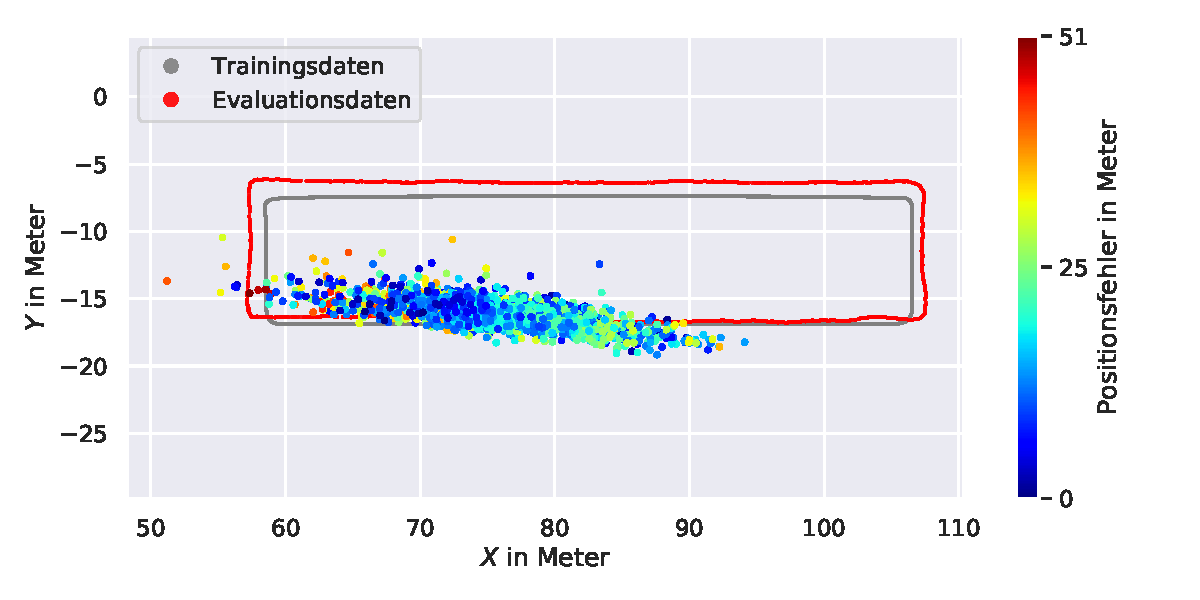
\includegraphics[width=1.0\linewidth]{images/results/ic_cycl/resultsfig_2.pdf} }\\
		\subcaption{} \label{subfig:ic_fig4} & \imagetop{ 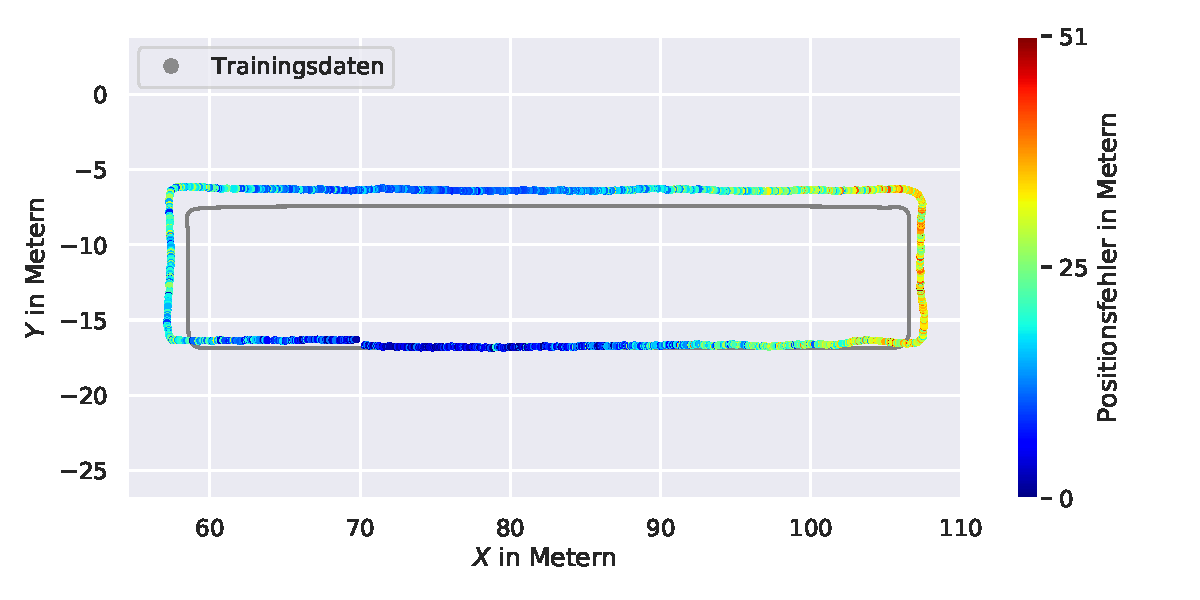
\includegraphics[width=1.0\linewidth]{images/results/ic_cycl/resultsfig_4.pdf} }\\
		\subcaption{} \label{subfig:ic_fig6} & \imagetop{ 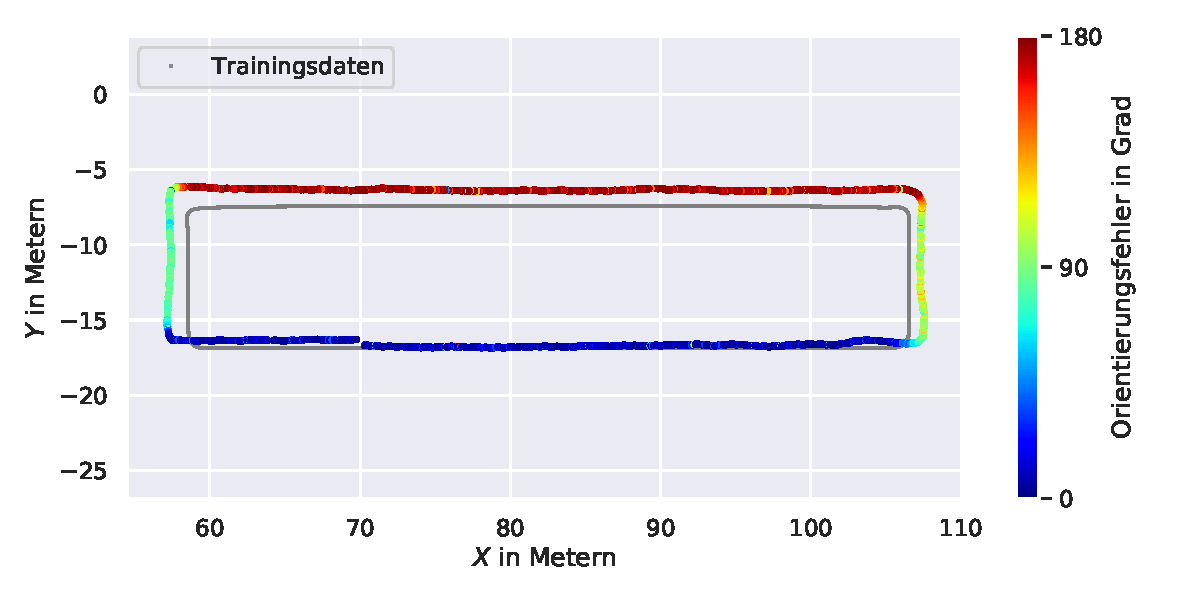
\includegraphics[width=1.0\linewidth]{images/results/ic_cycl/resultsfig_6.pdf} }\\
	\end{tabularx}
	\caption{Visualisierung der Evaluationsergebnisse von der Strecke \textit{IC-loop} (s. Abb. \ref{subfig:traj_ic}). Die Evaluation folgte mit den Gradietenbildern der realen Daten auf dem mit \textit{grad-photoreal} trainiertem Netzwerk. \subref{subfig:ic_fig2} illustriert die Positionen auf der xy-Ebene, die von dem KNN bestimmt wurden. Der Positionsfehler in der xy-Ebene und der Orientierungsfehler auf der Gierachse der jeweiligen Evaluationsdaten werden in  \subref{subfig:ic_fig4} und  \subref{subfig:ic_fig6} dargestellt.}
	\label{fig:result_ic_loop}
\end{figure}


\subsubsection{HS-gamma}


Ein weiteres Experiment folgte mit dem \textit{HS-gamma} Datensatz. Trainiert und Evaluiert mit nur synthetischen Daten konnte durch den \textit{grad-cartoon} Datensatz eine Akkuratesse von 1.00$m$ in der Position und 9.92° in der Orientierung erzielt werden (vgl. Tab. \ref{tab:results_hs_gamma}).  Dies stellt bei dem betroffenen Gebäudevolumen von $54m \times 10m \times 3m$ ein Potenzial zur Pose Estimation mit Daten der gleichen Beschaffenheit dar.

Die Evaluierung mit den \textit{grad-real} Evaluationsdaten auf dem mit \textit{grad-cartoon} trainiertem Netzwerk ergab eine Akkuratesse von 8.60$m$ in der Position und 19.59° in der Orientierung (vgl. Tab. \ref{tab:results_hs_gamma}). Bei oben genannten Gebäudemaßen ist eine Positionsgenauigkeit von 8.60$m$ sowie ein Orientierungsfehler von 19.59° unzureichend für die Bestimmung der Pose auf der \textit{HS-gamma} Strecke. Abbildung \ref{fig:result_hs_gamma} visualisiert die Evaluationsergebnisse von dem mit \textit{grad-cartoon} trainiertem und \textit{grad-real} evaluiertem Netzwerk.

Das mit \textit{grad-cartoon} trainierte Netzwerk bestimmte die Positionen aller \textit{grad-real} Evaluationsdaten nahe der erwähnten Schleife der \textit{HS-gamma} Strecke auf ein ca. 20$m$ langem Teilbereich (vgl. Abb.  \ref{subfig:hs_gamma_fig2}). Deshalb weisen die Evaluationsdaten nahe der Schleife die geringsten Positionsfehler auf. Zudem zeigen die Evaluationsdaten des zum Ausgangspunkt optisch ähnlichen Flures die größten Positionsfehlern auf (vgl. Abb. \ref{subfig:ic_fig4}). Ebenso bestimmte größtenteils das oben erwähnte Netzwerk die Orientierung der Evaluationsdaten als die Orientierung der dominierende Aufnahmerichtung. Daher sind die größten Orientierungsfehler bei den Evaluationsdaten der Schleife sowie der vertikal verlaufenden Strecke aufzufinden (vgl. Abb. \ref{subfig:ic_fig4}). 


\begin{table}
	\centering
	\caption{Evaluationsergebnisse von der Strecke \textit{HS-gamma}. Es wird die Akkuratesse der mit den jeweiligen Trainingsdaten trainierten Netzwerke angegeben, die mit den korrespondierenden synthetischen Evaluationsdaten sowie jeweils mit den realen Evaluationsdaten evaluiert wurden.}
	\begin{tabularx}{1.0\textwidth}{X >{\RaggedRight}X >{\RaggedRight}X}
	\textbf{Trainingsdatensatz} \hspace{2cm} (Gradientenbild) & \textbf{synthetische Daten} \hspace{2cm} (Position, Orientierung) & \textbf{reale Daten} \hspace{2cm} (Position, Orientierung)\\
	\hline
		\textit{grad-cartoon} & 1.00$m$, 9.92° & 8.60$m$, 19.59°\\
		\hline
		\textit{grad-edge} & 1.07$m$, 8.69° & 10.15$m$, 35.11°\\
		\hline
		\textit{grad-photoreal} & 1.45$m$, 9.17° & 10.27$m$, 41.60°\\
	\end{tabularx}
	\label{tab:results_hs_gamma}
\end{table}

\begin{figure}
	\setlength\extrarowheight{-15pt}
	\centering
	\begin{tabularx}{0.9\textwidth}{>{\centering\arraybackslash}p{0.05\textwidth} X}
		\subcaption{} \label{subfig:hs_gamma_fig2} & \imagetop{ 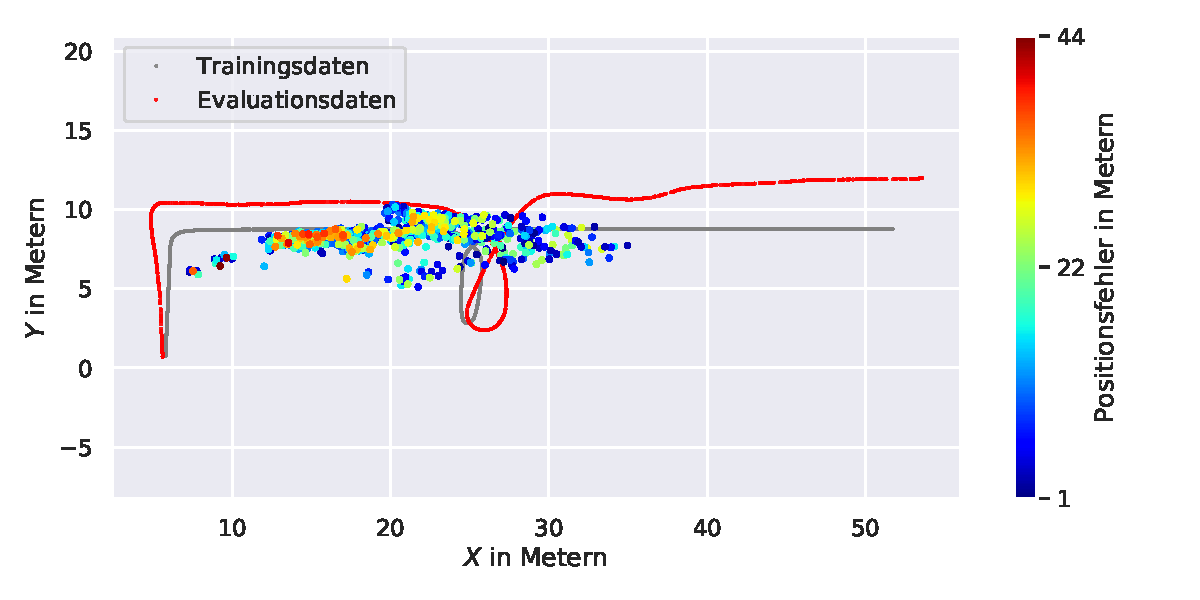
\includegraphics[width=1.0\linewidth]{images/results/hs_gamma/resultsfig_2.pdf} }\\
		\subcaption{} \label{subfig:hs_gamma_fig4} & \imagetop{ 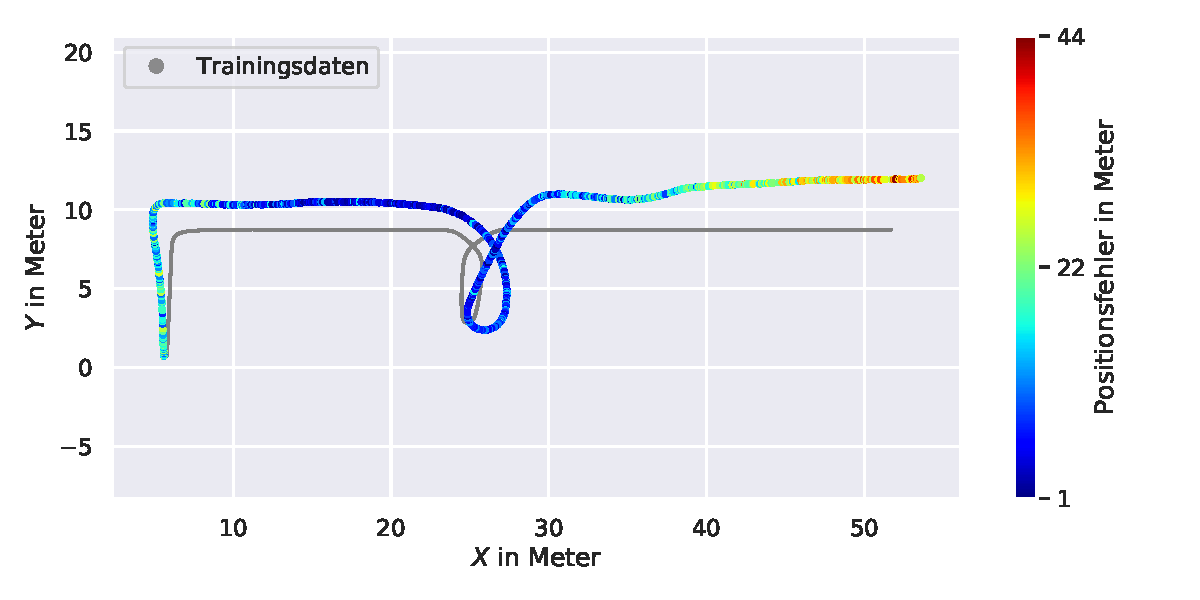
\includegraphics[width=1.0\linewidth]{images/results/hs_gamma/resultsfig_4.pdf} }\\
		\subcaption{} \label{subfig:hs_gamma_fig6} & \imagetop{ 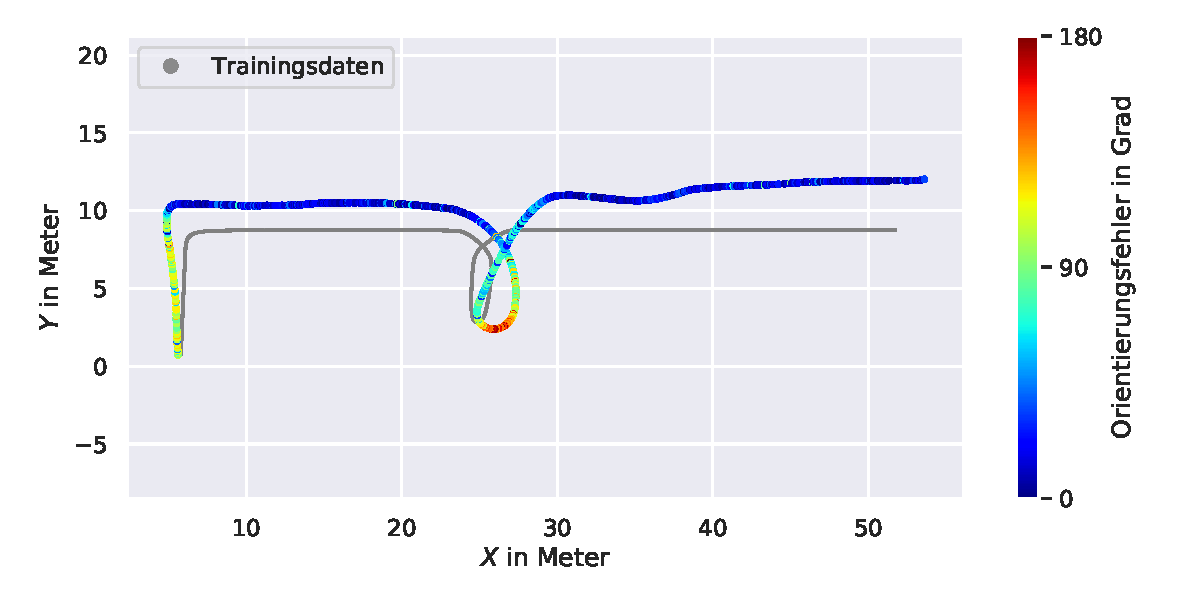
\includegraphics[width=1.0\linewidth]{images/results/hs_gamma/resultsfig_6.pdf} }\\
	\end{tabularx}
	\caption{Visualisierung der Evaluationsergebnisse von der Strecke \textit{HS-gamma} (s. Abb. \ref{subfig:traj_hs_gamma}). Die Evaluation folgte mit den Gradietenbildern der realen Daten auf dem mit \textit{grad-cartoon} trainiertem Netzwerk. \subref{subfig:hs_gamma_fig2} illustriert die Positionen auf der xy-Ebene, die von dem KNN bestimmt wurden. Der Positionsfehler in der xy-Ebene und der Orientierungsfehler auf der Gierachse der jeweiligen Evaluationsdaten werden in  \subref{subfig:hs_gamma_fig4} und  \subref{subfig:hs_gamma_fig6} dargestellt.}
	\label{fig:result_hs_gamma}
\end{figure}

\subsubsection{HS-stairs-up}
Weiterhin wurde ein Experiment mit dem \textit{HS-stairs-up} Datensatz durchgeführt. Ausschließlich mit synthetischen Daten konnte eine Akkuratesse von 0.82$m$ in der Position und 7.76° in der Orientierung durch die \textit{grad-cartoon} Daten erzielt werden (vgl. Tab. \ref{tab:results_hs_stairs_up}). besitzt dieses Experiment ebenso das Potenzial zur Pose Estimation.

Bei der Evaluierung, mit den \textit{grad-real} Evaluationsdaten, konnte eine Akkuratesse von 4.33$m$ in der Position und 51.64° in der Orientierung durch das mit \textit{grad-edge} trainierte Netzwerk erreicht werden. Sowohl ein Positionsfehler von 4.33$m$ als auch ein Orientierungsfehler von 51.64°  sind für die Bestimmung der Pose in einem ca. $12m \times 12m \times 12m$ großen Zone ungenügend.


\begin{table}
	\centering
	\caption{Evaluationsergebnisse von der Strecke \textit{HS-stairs-up} (s. Abb. \ref{subfig:traj_hs-up}). Es wird die Akkuratesse der mit den jeweiligen Trainingsdaten trainierten Netzwerke angegeben, die mit den korrespondierenden synthetischen Evaluationsdaten sowie jeweils mit den realen Evaluationsdaten evaluiert wurden.}
	\begin{tabularx}{1.0\textwidth}{X >{\RaggedRight}X >{\RaggedRight}X}
		\textbf{Trainingsdatensatz} \hspace{2cm} (Gradientenbild) & \textbf{synthetische Daten} \hspace{2cm} (Position, Orientierung) & \textbf{reale Daten} \hspace{2cm} (Position, Orientierung)\\
		\hline
		\textit{grad-cartoon} & 0.82$m$, 7.76° & 4.77$m$, 23.43°\\
		\hline
		\textit{grad-edge} & 0.82$m$, 8.48° & 4.33$m$, 51.64°\\
		\hline
		\textit{grad-photoreal} & 0.92$m$, 7.98° & 5.16$m$, 93.38°\\
	\end{tabularx}
	\label{tab:results_hs_stairs_up}
\end{table}


\begin{figure}
	\setlength\extrarowheight{-15pt}
	\centering
	\begin{tabularx}{0.9\textwidth}{>{\centering\arraybackslash}p{0.05\textwidth} X}
		\subcaption{} \label{subfig:hs_up_fig3} & \imagetop{ 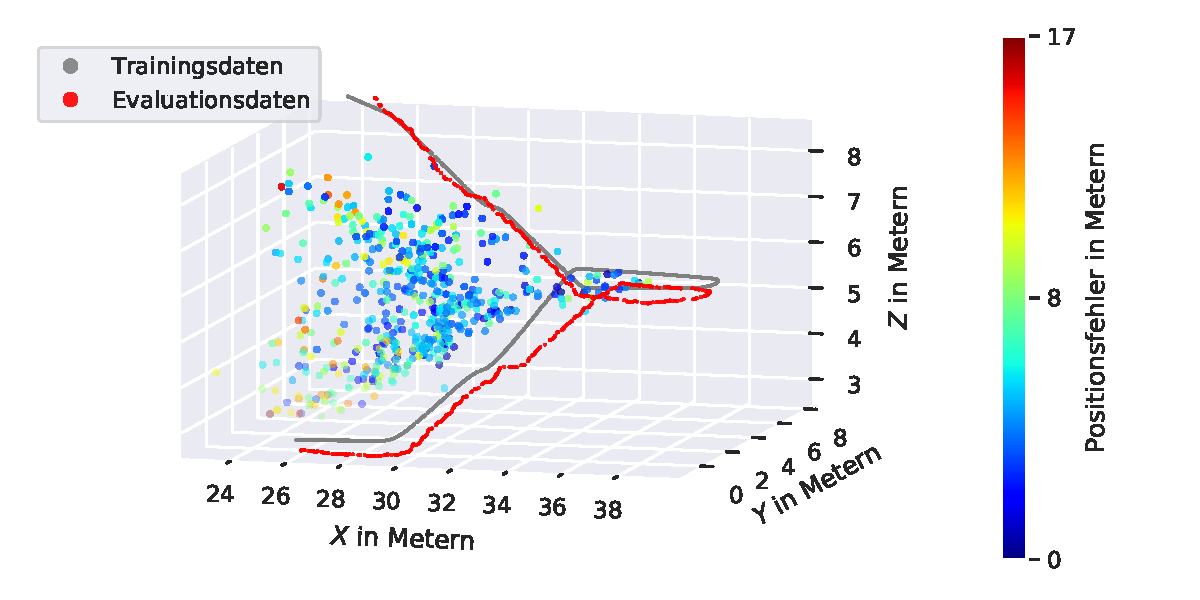
\includegraphics[width=1.0\linewidth]{images/results/hs_up/resultsfig_3.pdf} }\\
		\subcaption{} \label{subfig:hs_up_fig5} & \imagetop{ 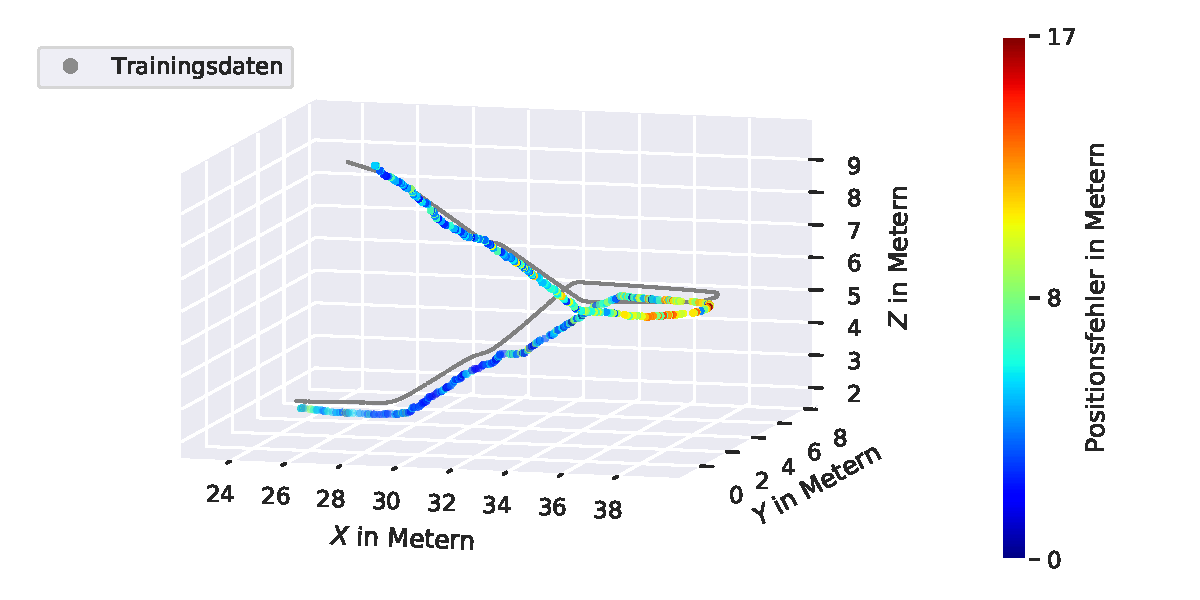
\includegraphics[width=1.0\linewidth]{images/results/hs_up/resultsfig_5.pdf} }\\
		\subcaption{} \label{subfig:hs_up_fig7} & \imagetop{ 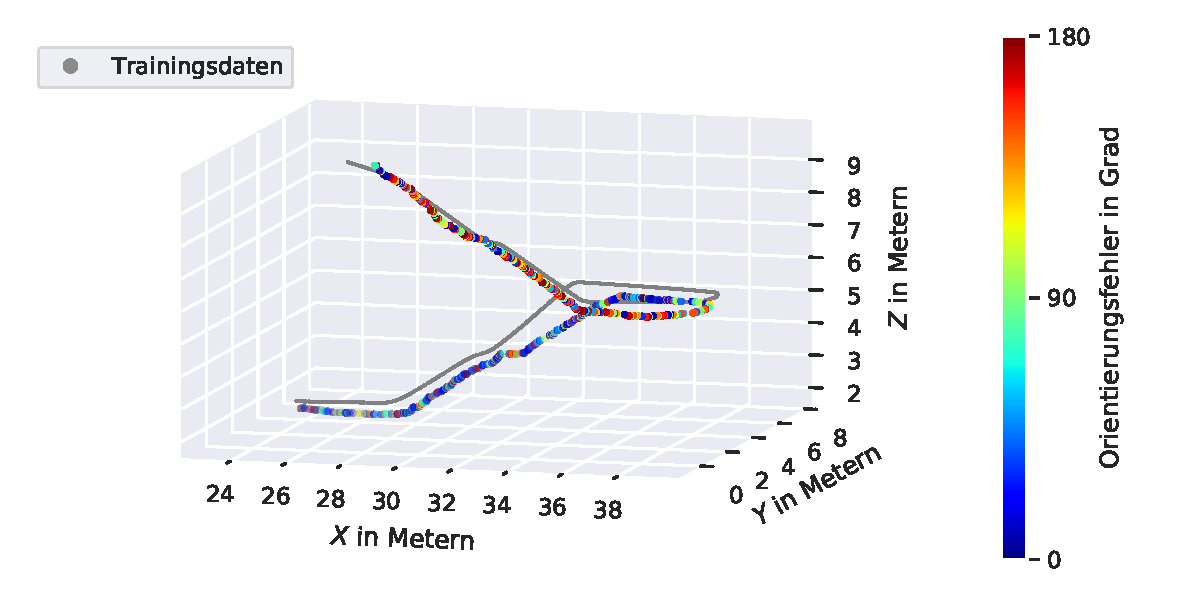
\includegraphics[width=1.0\linewidth]{images/results/hs_up/resultsfig_7.pdf} }\\
	\end{tabularx}
	\caption{Visualisierung der Evaluationsergebnisse von der Strecke \textit{HS-stairs-up}. Die Evaluation folgte mit den Gradietenbildern der realen Daten auf dem mit \textit{grad-edge} trainiertem Netzwerk. \subref{subfig:hs_up_fig3} illustriert die Positionen auf der xy-Ebene, die von dem KNN bestimmt wurden. Der Positionsfehler in der xy-Ebene und der Orientierungsfehler auf der Gierachse der jeweiligen Evaluationsdaten werden in  \subref{subfig:hs_up_fig5} und  \subref{subfig:hs_up_fig7} dargestellt.}
	\label{fig:result_hs_stairs_up}
\end{figure}


\subsubsection{HS-stairs-down}
 Mit ausschließlich den Gradietenbilder der synthetischen Kantenbildern konnte eine Akkuratesse von 0.85$m$ in der Position und 7.50° in der Orientierun erreicht werden. Bei der Evaluierung mit den Gradientenbildern der realen Daten konnte eine Akkuratesse von 4.20$m$ in der Position und 47.83° in der Orientierung auf dem Netzwerk erreicht werden, der mit den Gradietenbilder der karikaturistische Simulation trainiert wurde. Abbildung \ref{fig:result_hs_stairs_down} visualisiert die Evaluierungsergebnisse von diesem künstlichen neuronalen Netzwerk.
\begin{table}
	\centering
	\caption{Evaluationsergebnisse von der Strecke \textit{HS-stairs-down} (s. Abb. \ref{subfig:traj_hs-down}). Es wird die Akkuratesse der mit den jeweiligen Trainingsdaten trainierten Netzwerke angegeben, die mit den korrespondierenden synthetischen Evaluationsdaten sowie jeweils mit den realen Evaluationsdaten evaluiert wurden.}
	\begin{tabularx}{1.0\textwidth}{X >{\RaggedRight}X >{\RaggedRight}X}
		\textbf{Trainingsdatensatz} \hspace{2cm} (Gradientenbild) & \textbf{synthetische Daten} \hspace{2cm} (Position, Orientierung) & \textbf{reale Daten} \hspace{2cm} (Position, Orientierung)\\
		\hline
		\textit{grad-cartoon} & 0.91$m$, 8.01° & 4.20$m$, 47.83°\\
		\hline
		\textit{grad-edge} & 0.85$m$, 7.50° & 5.59$m$, 67.34°\\
		\hline
		\textit{grad-photoreal} & 1.02$m$, 8.57° & 5.25$m$, 32.70°\\
	\end{tabularx}
	\label{tab:results_hs_stairs_down}
\end{table}


\begin{figure}
	\setlength\extrarowheight{-15pt}
	\centering
	\begin{tabularx}{0.9\textwidth}{>{\centering\arraybackslash}p{0.05\textwidth} X}
		\subcaption{} \label{subfig:hs_down_fig3} & \imagetop{ 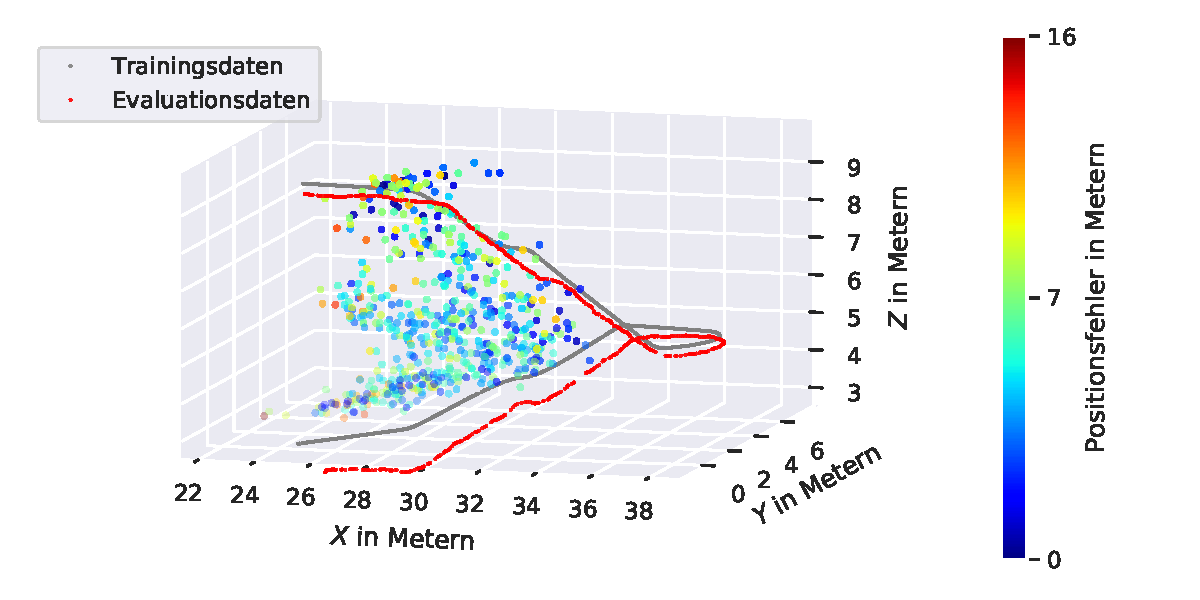
\includegraphics[width=1.0\linewidth]{images/results/hs_down/resultsfig_3.pdf} }\\
		\subcaption{} \label{subfig:hs_down_fig5} & \imagetop{ 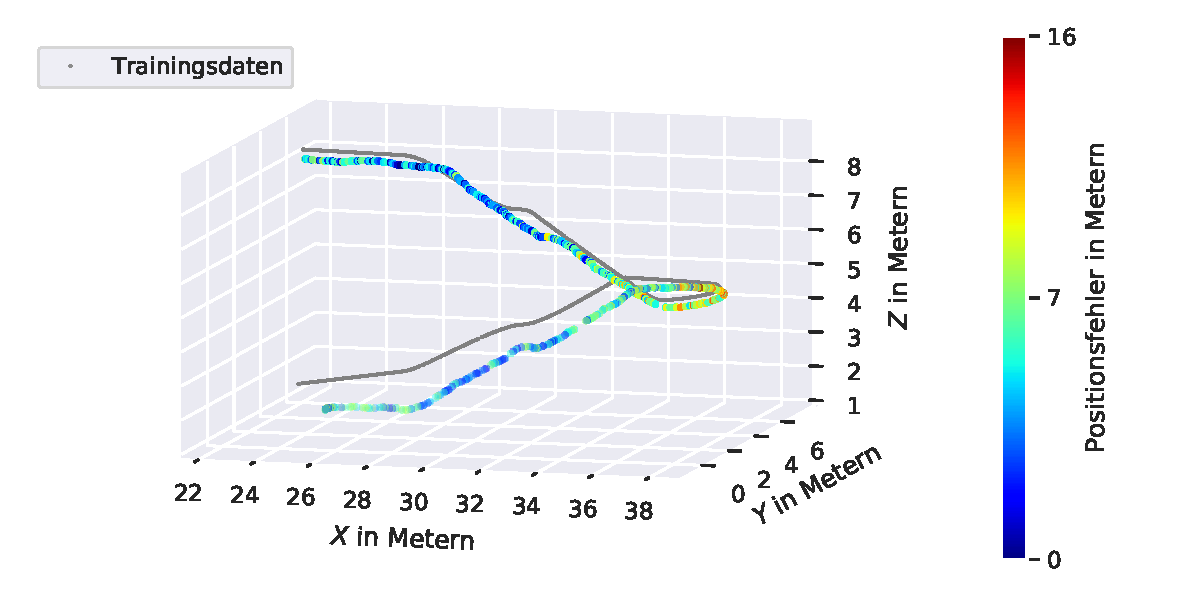
\includegraphics[width=1.0\linewidth]{images/results/hs_down/resultsfig_5.pdf} }\\
		\subcaption{} \label{subfig:hs_down_fig7} & \imagetop{ 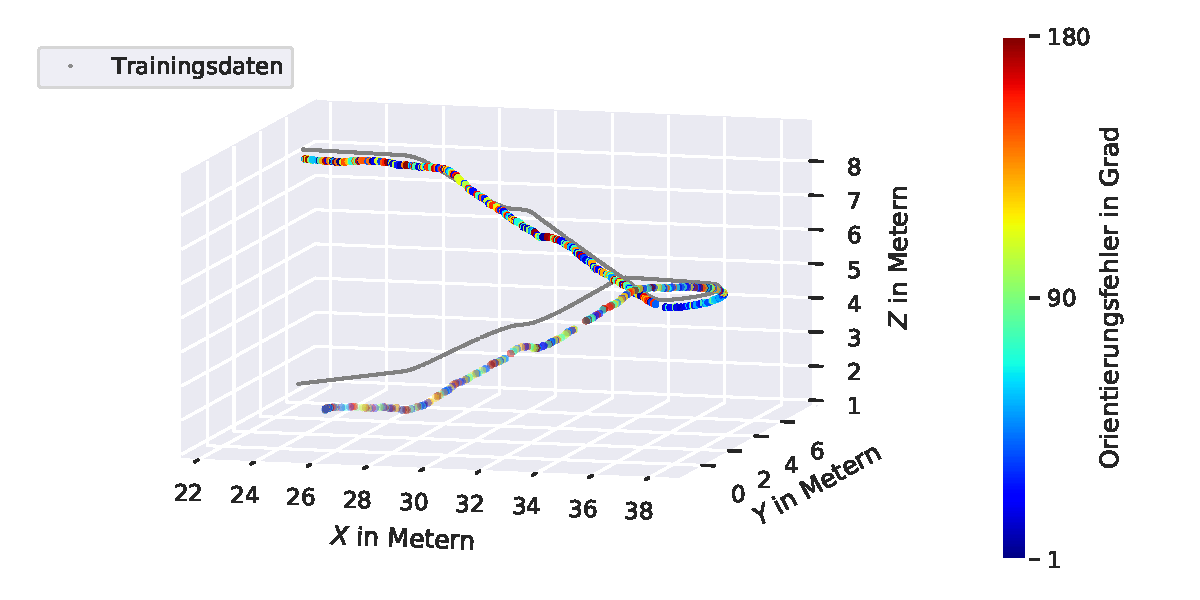
\includegraphics[width=1.0\linewidth]{images/results/hs_down/resultsfig_7.pdf} }\\
	\end{tabularx}
	\caption{Visualisierung der Evaluationsergebnisse von der Strecke \textit{HS-stairs-up}. Die Evaluation folgte mit den Gradietenbildern der realen Daten auf dem mit \textit{grad-cartoon} trainiertem Netzwerk. \subref{subfig:hs_down_fig3} illustriert die Positionen auf der xy-Ebene, die von dem KNN bestimmt wurden. Der Positionsfehler in der xy-Ebene und der Orientierungsfehler auf der Gierachse der jeweiligen Evaluationsdaten werden in  \subref{subfig:hs_down_fig5} und  \subref{subfig:hs_down_fig7} dargestellt.}
	\label{fig:result_hs_stairs_down}
\end{figure}






% !TEX root = ../my_thesis.tex

\section{Diskussion}
\label{sec:kapitel_5}
Die Ergebnisse der Forschungen haben gezeigt, dass der Ansatz von \citet{acharyaBIMPoseNetIndoorCamera2019} ohne weiteren Regelungen, auf die im Rahmen dieser Bachelorarbeit erhobenen Datensätze, nutzlose Resultate erzielt.
% !TEX root = ../my_thesis.tex

\section{Fazit}
\label{sec:kapitel_6}
Das Ziel dieser Bachelorarbeit war, den Ansatz von \citet{acharyaBIMPoseNetIndoorCamera2019} zur Pose Estimation anhand von Convolutional Neural Networks und simulierten 3D-Daten in größeren Gebäudesimulationen und auf längeren Strecken zu untersuchen.
Insgesamt wurde der Ansatz in zwei unterschiedlichen Gebäuden auf vier Strecken untersucht. Zusammenfassend konnte durch die Untersuchungen festgestellt werden, dass ein Lokalisierungsverfahren über den Ansatz von \citet{acharyaBIMPoseNetIndoorCamera2019} mit den hier erhobenen Datensätzen nicht möglich ist.


Eine Akkuratesse von ca. 1$m$ in der Position und 8° in der Orientierung konnte durch die zugrundeliegende CNN PoseNet mit Daten der gleichen Domäne in der Trainings- und Evaluationsphase erzielt werden. Im Gegensatz dazu konnte bei domänenübergreifender Anwendung eine durchschnittlichen Akkuratesse von 10.95$m$, 49.69° erreicht werden. Hierbei konnte PoseNet nur auf einem begrenzten Gebäudeareal in einer Richtung trainiert werden. Dies zeigte Parallelen zu den Ergebnissen von \citet{acharyaBIMPoseNetIndoorCamera2019}, da diese PoseNet auf einer überwiegend in eine Richtung verlaufenden Strecke in einem kleinem Korridor trainierten. Angesichts dieser Parallelen lag die Schlussfolgerung nahe, dass durch das Trainieren mit den Gradientenbildern der synthetischen Daten bei gleichen Hyperparametern wie in \cite{acharyaBIMPoseNetIndoorCamera2019} von PoseNet die Gradientenbilder der realen Evaluationsdaten auf einem begrenzten Gebäudeareal nur in eine Richtung bestimmt werden können.

% Motivieren
Eine mögliche Positionsakkuratesse von 1$m$ ist im strengen Sinne unzureichend für Anwendungen wie die automatische Bauforstschritterfassung sowie das Facility-Management und die Navigation über Augmented Reality.

% OUTLOOK

Die Verschlechterung der Ergebnisse bei domänenübergreifender Anwendung lassen sich auf die strukturellen Unterschiede der Realität zur Simulationsumgebung wie z.B. das Fehlen von diversen Objekten und das Vorhanden sein von domänenspezifischen Artefakten zurückführen. Die Diskrepanzminimierung durch \textit{Generative Adversarial Networks} von synthetischen Datensätze zu den realen Datensätzen könnte zu besseren Ergebnissen führen. Ferner könnte ein Fortschritt durch Beschränkungen der möglichen Posen im Trainingsprozess erzielt werden, sodass die Positionsergebnisse immer in den begehbaren Innenräumen der Gebäuden abgebildet werden.


\end{document}
